% !TEX encoding = UTF-8 Unicode

% Compilation using 'acmsmall.cls' - version 1.3 (March 2012), Aptara Inc.
% (c) 2010 Association for Computing Machinery (ACM)
%
% Questions/Suggestions/Feedback should be addressed to => "acmtexsupport@aptaracorp.com".
% Users can also go through the FAQs available on the journal's submission webpage.
%
% Steps to compile: latex, bibtex, latex, latex


\documentclass[prodmode,acmtochi]{acmsmall} % Aptara syntax

% Package to generate and customize Algorithm as per ACM style
\usepackage[ruled]{algorithm2e}
\renewcommand{\algorithmcfname}{ALGORITHM}
\SetAlFnt{\small}
\SetAlCapFnt{\small}
\SetAlCapNameFnt{\small}
\SetAlCapHSkip{0pt}
\IncMargin{-\parindent}

% Packages
\usepackage[super]{nth}
\usepackage[inline]{enumitem}
\usepackage{moreenum}
\usepackage{tabulary}
\usepackage{tabu}
\usepackage{booktabs}
\usepackage{array}
\usepackage[super]{nth}
\usepackage{listings}
\usepackage{float}
\usepackage{tikz}
\usepackage{upquote}
%\usepackage{minted}
%\usemintedstyle{bw}
\newcommand{\ra}[1]{\renewcommand{\arraystretch}{#1}}
%\newcommand{\urlhttp}[1]{\href{http://#1}{\nolinkurl{#1}}}
%\newcommand{\urlhttps}[1]{\href{https://#1}{\nolinkurl{#1}}}

% Special characters
\usepackage{gensymb}
\usepackage{amssymb}
\usepackage{pifont}
\newcommand{\cmark}{\ding{51}}
\newcommand{\xmark}{\ding{55}}

% Fix table of contents
\makeatletter
\newcommand\l@paragraph[2]{}
\newcommand\l@subparagraph[2]{}
\makeatother

% Metadata Information
\acmVolume{0}
\acmNumber{0}
\acmArticle{0}
\acmYear{0}
\acmMonth{0}

% Copyright
%\setcopyright{acmcopyright}
%\setcopyright{acmlicensed}
%\setcopyright{rightsretained}
%\setcopyright{usgov}
%\setcopyright{usgovmixed}
%\setcopyright{cagov}
%\setcopyright{cagovmixed}

% DOI
\doi{0000001.0000001}

%ISSN
\issn{1234-56789}

% Document starts
\begin{document}

% Page heads
\markboth{B. Harmon et al.}{Cognitively Grasping Topography with Tangible Landscape}

% Title portion
\title{Cognitively Grasping Topography with Tangible Landscape} 
% Cognitively Grasping 3D Form with Tangible Landscape
% Multidimensional Sketching with Tangible Landscape
% Embodied Spatial Cognition in Tangible Computing
% Cognitively Grasping Topography with Tangible Landscape
% Tangible Landscape: Cognitively Grasping Topography
% Tangible Landscape: a Tangible Interface for Geospatial Modeling
% Tangible Landscape: Cognitively Grasping Topography with a Tangible Interface for Geospatial Modeling
% Tangible Landscape: a 3D Sketching with a Tangible Interface for Geospatial Modeling
% 
\author{BRENDAN ALEXANDER HARMON
\affil{North Carolina State University}
ANNA PETRASOVA
\affil{North Carolina State University}
VACLAV PETRAS
\affil{North Carolina State University}
HELENA MITASOVA
\affil{North Carolina State University}
ROSS ​KENDALL MEENTEMEYER
\affil{North Carolina State University}
EUGENE BRESSLER
\affil{North Carolina State University}
ART RICE
\affil{North Carolina State University}}

\begin{abstract}
%
%Spatial thinking can be embodied 
%-- people can functionally think about space with their bodies 
%by kinaesthetically experiencing space, 
%cognitively grasping objects, and 
%physically simulating spatial transformations.
%
Tangible interfaces for spatial modeling
combine embodied, kinaesthetic interaction with spatial computations. 
%
Theoretically this should enable users to 
intuitively interact 
with multidimensional digital models of space,
offloading challenging cognitive tasks onto the body and 
computationally enhancing how they think about space.
% 
We have designed Tangible Landscape 
-- a tangible interface powered by a geographic information system (GIS) 
that gives 3D spatial data an interactive, physical form so that 
users can naturally sense and shape it.
%
Tangible Landscape couples a physical and a digital model of a landscape
through real-time cycles of 
physical manipulation, 3D scanning, spatial computation, and projected feedback.
%
%As users manipulate
%a physical model of a landscape
%the model is 3D scanned, the scan is imported into GIS 
%for spatial modeling, analysis, and simulation, 
%and the results are projected back onto the model.
%
Through a series of 
3D modeling experiments 
assessed using both
quantitative %methods 
%such as geospatial modeling
and qualitative methods 
%such as geospatial modeling and interviews
%including semi-structured interviews and direct observation
%to study how Tangible Landscape
%mediates 3D spatial performance.
%
%We determined that tangible interfaces for geospatial modeling 
%can improve 3D spatial performance.
we determined that Tangible Landscape 
can improve 3D spatial performance. 
%
The participants produced more accurate models 
that better represented morphological features 
with tangible modeling than they did with either digital or analog, hand modeling. 



\end{abstract}

%
% The code below should be generated by the tool at
% http://dl.acm.org/ccs.cfm
% Please copy and paste the code instead of the example below. 
%
\begin{CCSXML}
<ccs2012>
<concept>
<concept_id>10003120.10003121</concept_id>
<concept_desc>Human-centered computing~Human computer interaction (HCI)</concept_desc>
<concept_significance>500</concept_significance>
</concept>
<concept>
<concept_id>10003120.10003121.10003122.10011749</concept_id>
<concept_desc>Human-centered computing~Laboratory experiments</concept_desc>
<concept_significance>500</concept_significance>
</concept>
</ccs2012>
\end{CCSXML}

\ccsdesc[500]{Human-centered computing~Human computer interaction (HCI)}
\ccsdesc[500]{Human-centered computing~Laboratory experiments}
%
% End generated code
%

\keywords{Human-computer interaction, tangible interfaces, interaction design, physical computation, embodied cognition, spatial thinking, geospatial modeling}

\acmformat{Brendan A. Harmon, Anna Petrasova, Vaclav Petras, Helena Mitasova, Ross K. Meentemeyer, Eugene H. Bressler, and Art Rice, 2016. Cognitively Grasping Topography with Tangible Landscape.}

\begin{bottomstuff}
Author's addresses: B. A. Harmon {and} A. Petrasova {and} V. Petras {and} H. Mitasova {and} R. K. Meentemeyer, Center for Geospatial Analytics, North Carolina State University; B. A. Harmon, E. H. Bressler {and} A. Rice, Department of Landscape Architecture, North Carolina State University.
\end{bottomstuff}


\maketitle

%{\tableofcontents}
%{\listoffigures}
%{\listoftables}

\section{Introduction}

\begin{figure}
\begin{center}
%		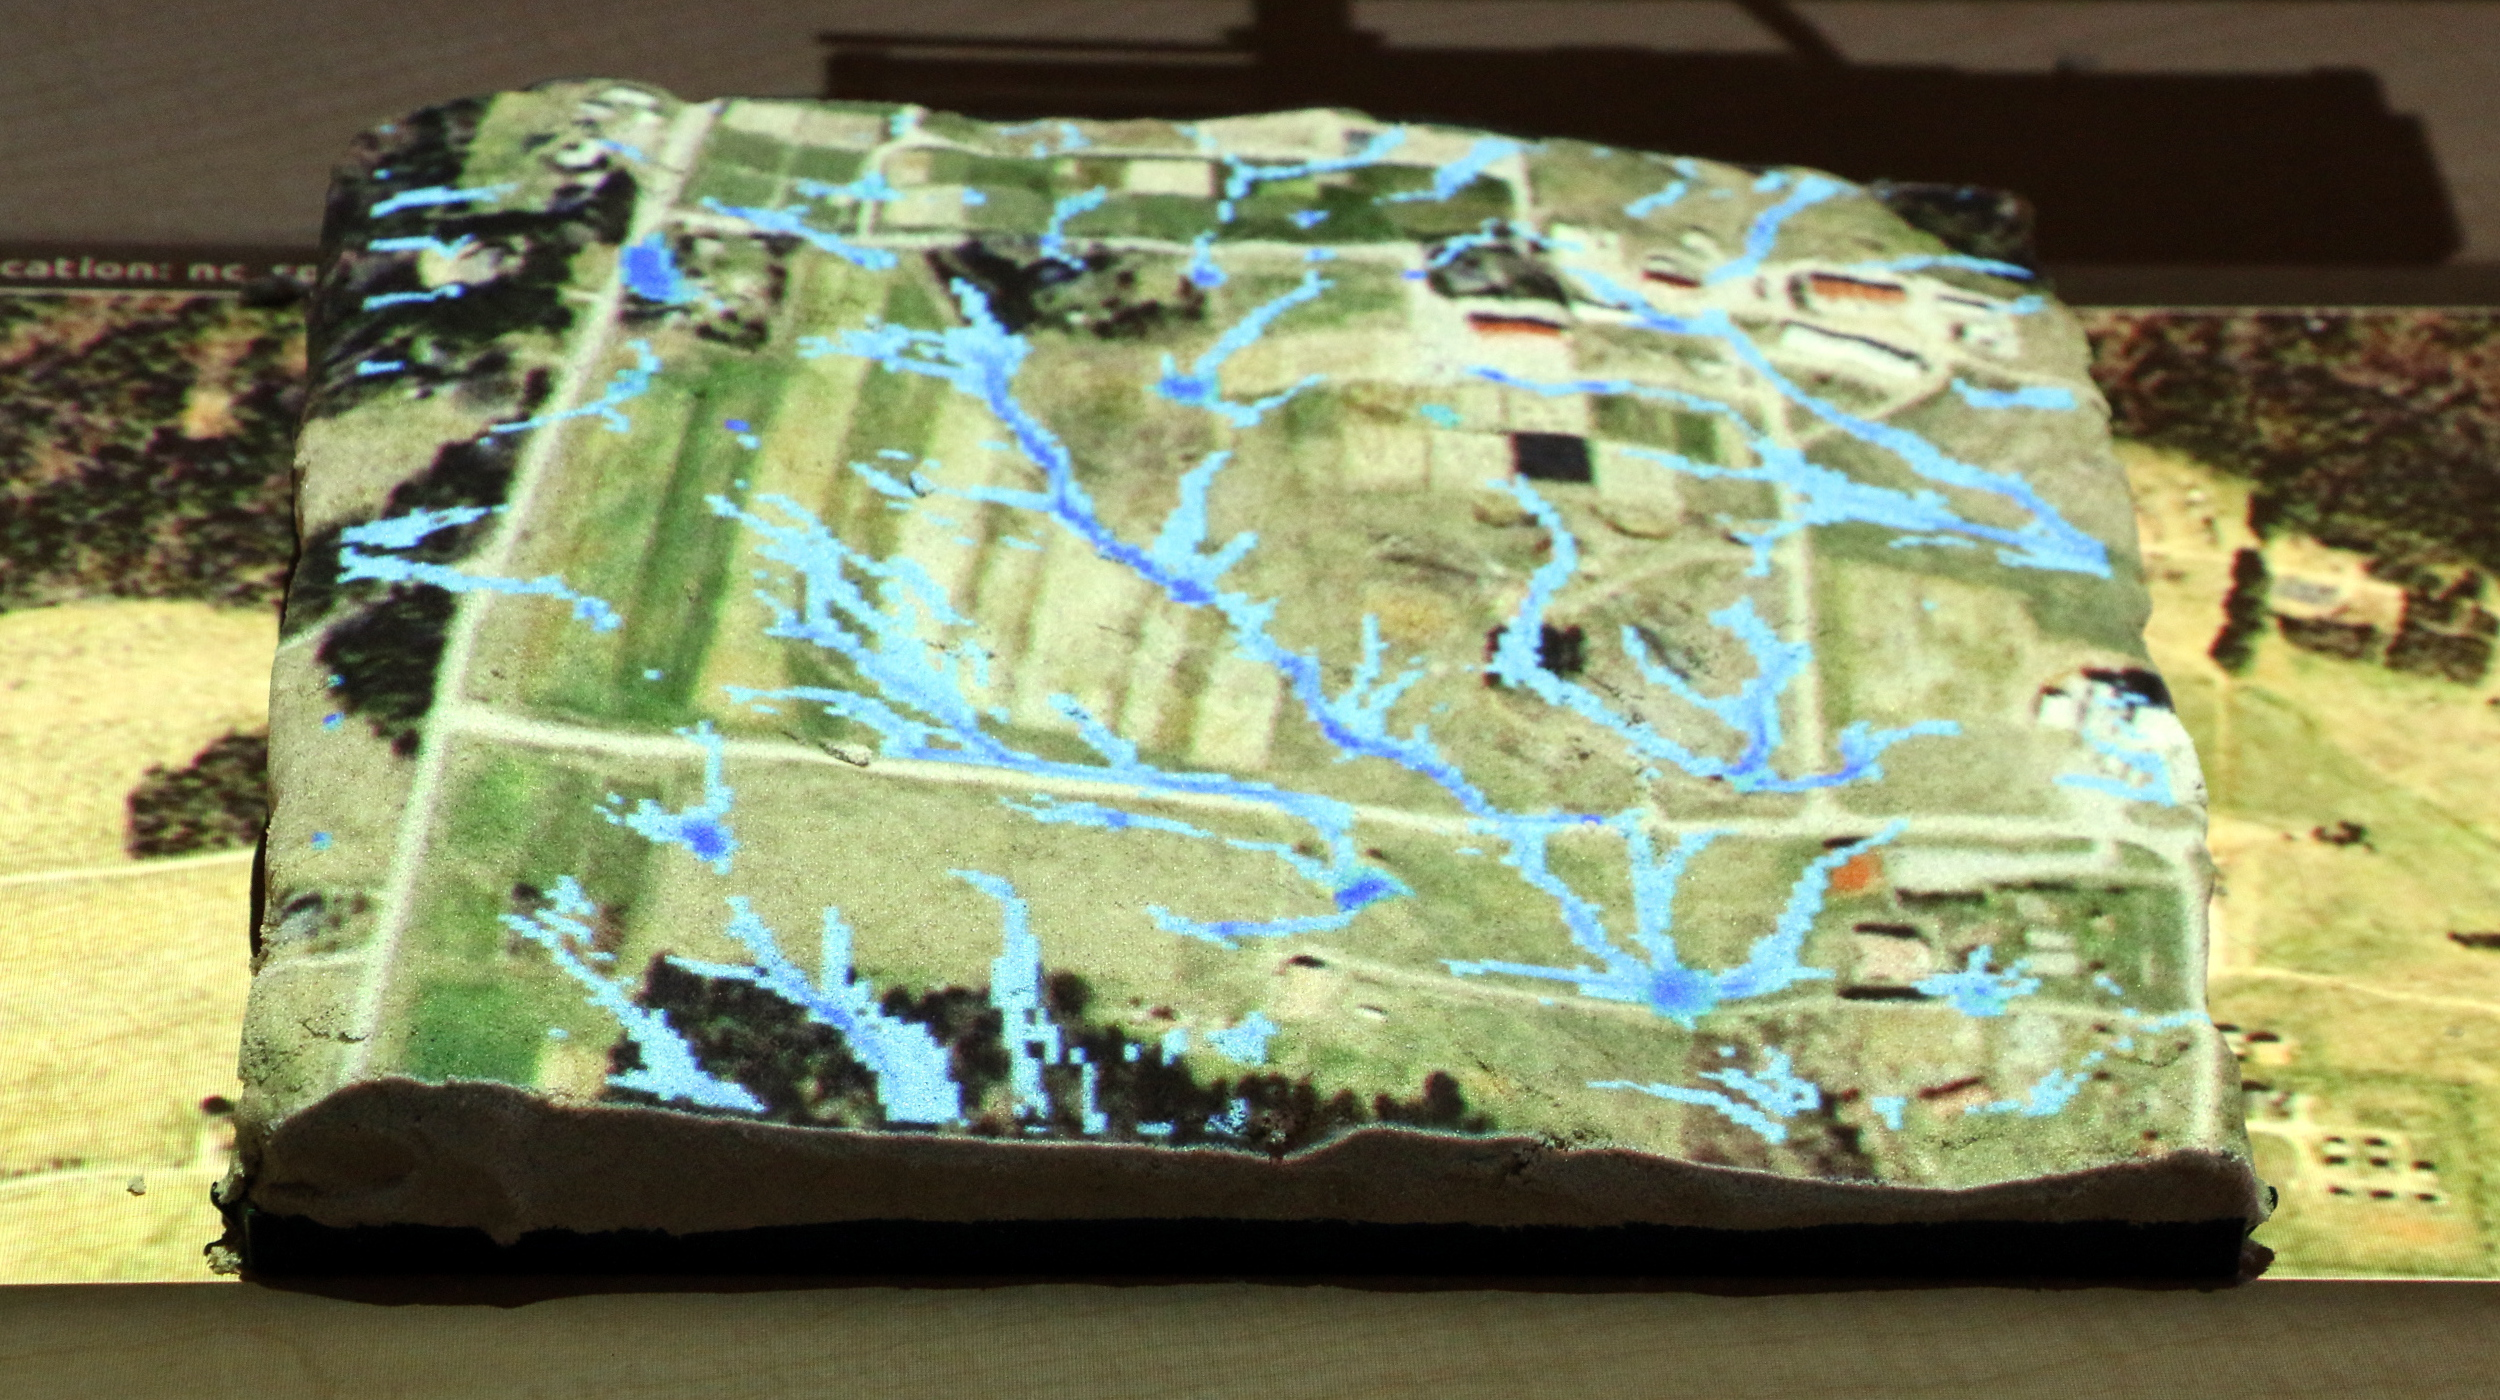
\includegraphics[width=0.32\textwidth]{images/applications/tl_sequence_1.jpg}
		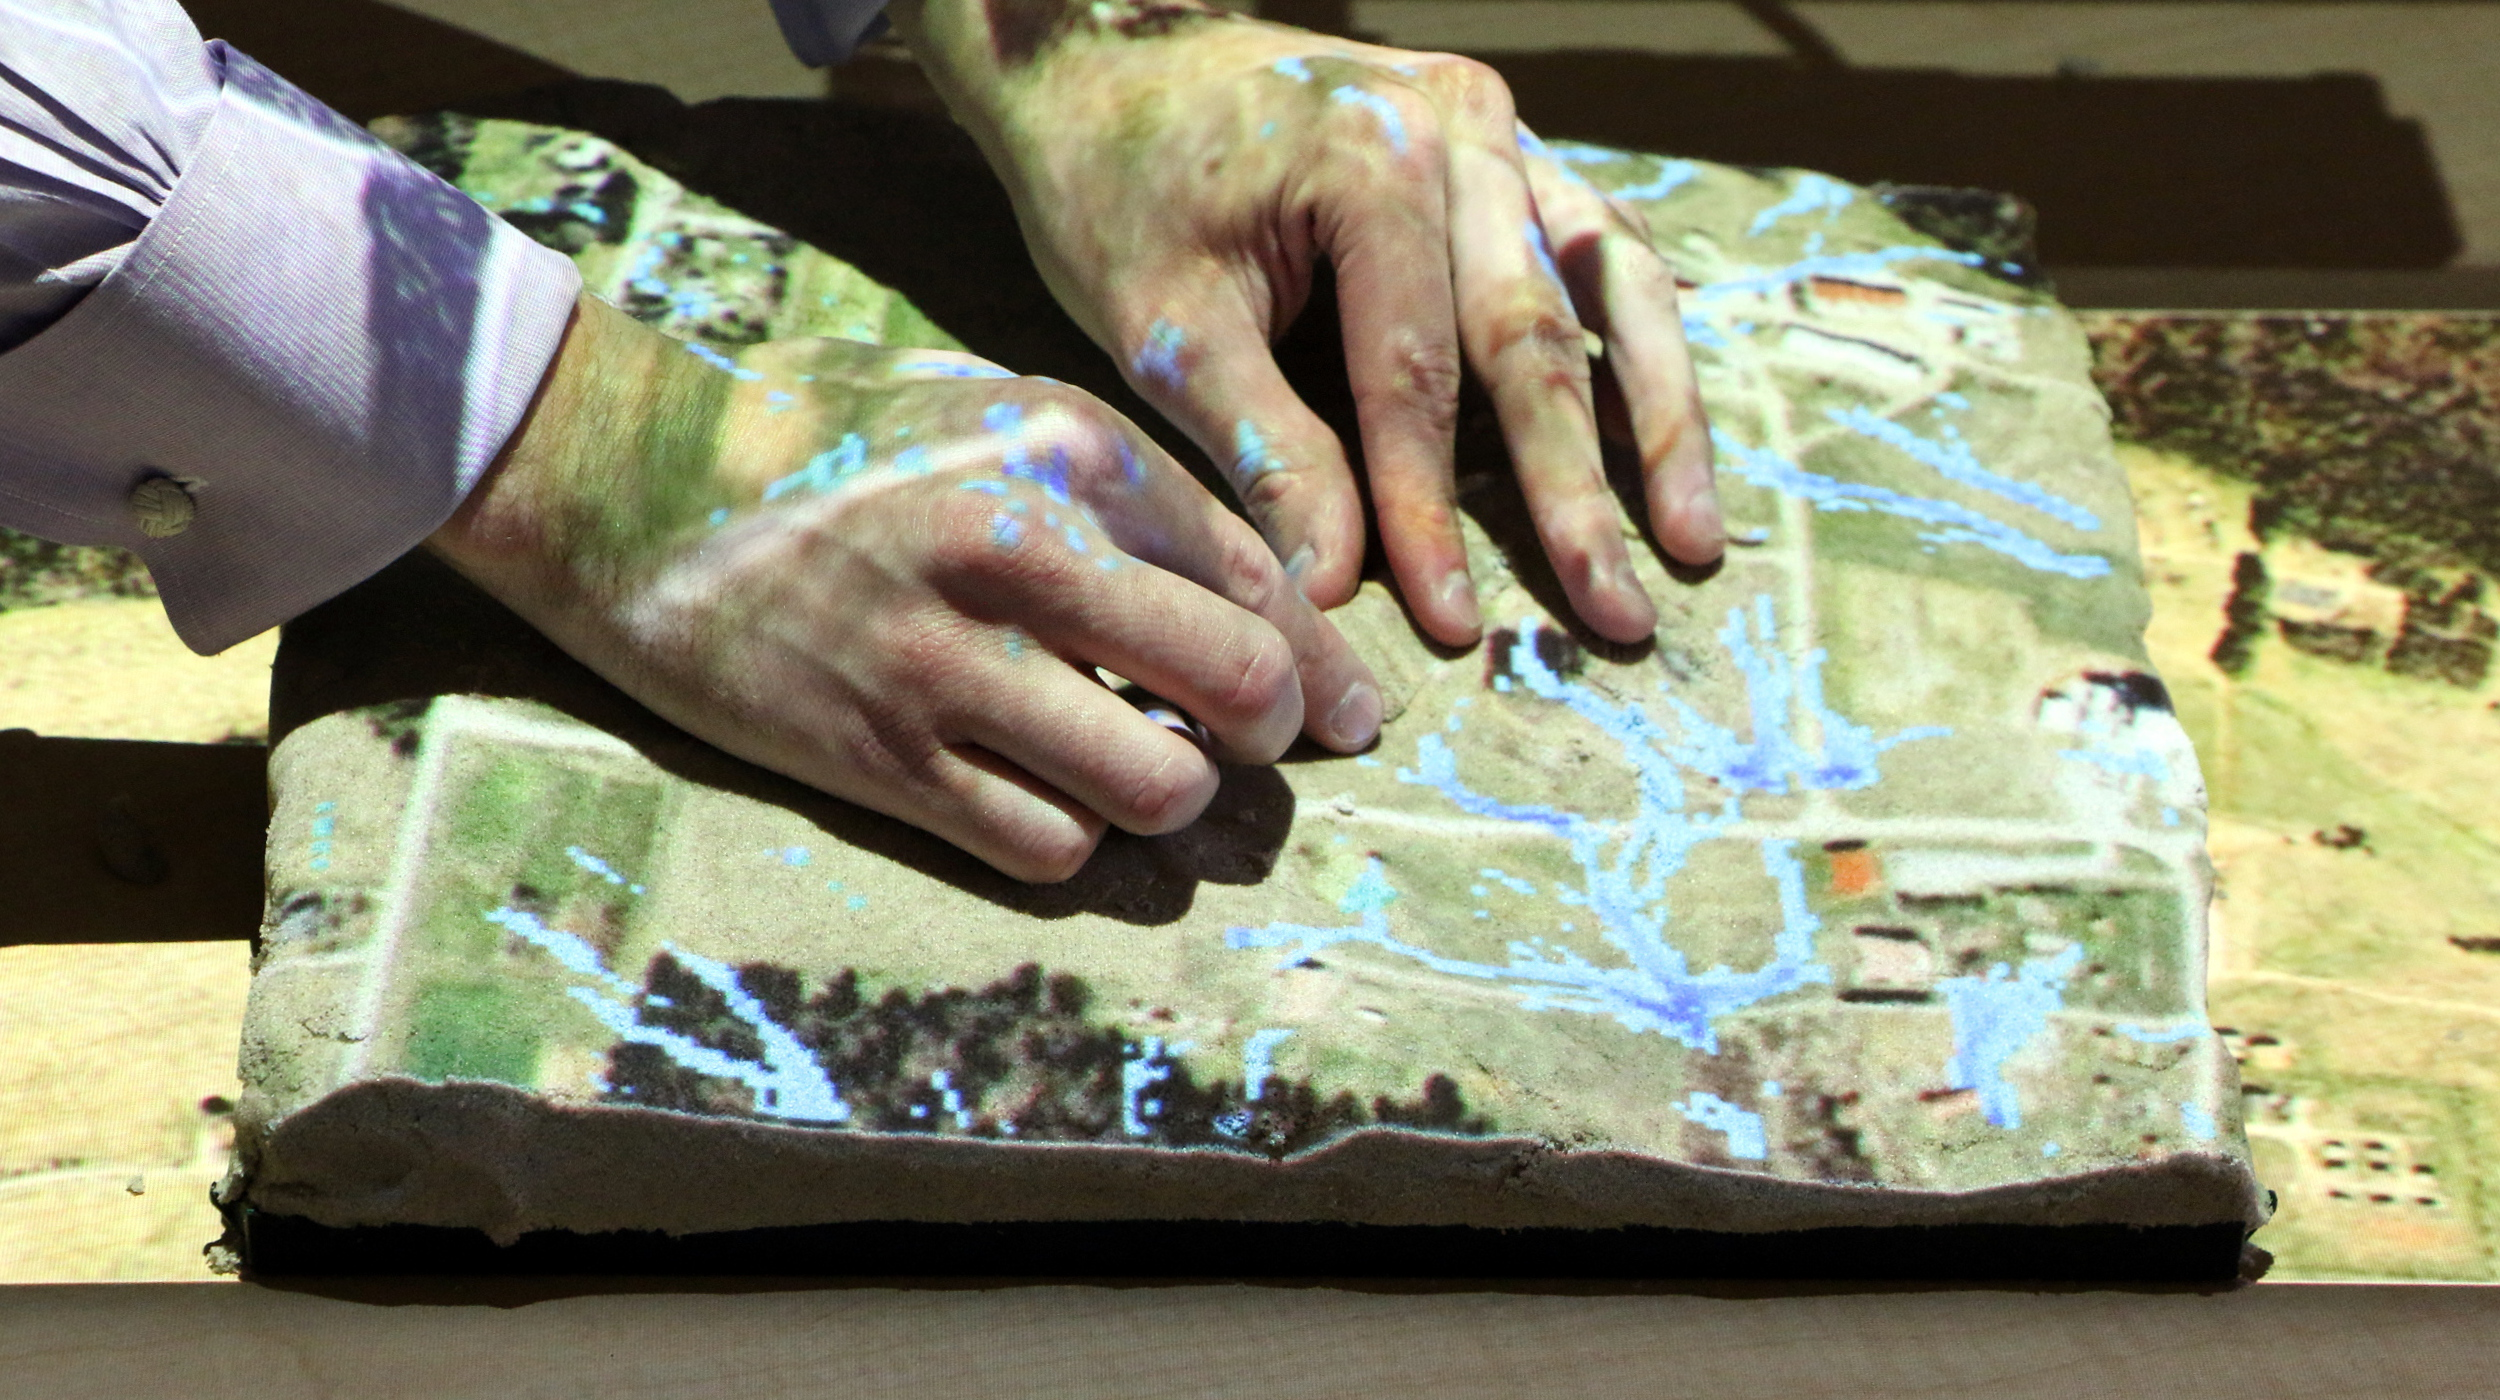
\includegraphics[width=0.49\textwidth]{images/applications/tl_sequence_2.jpg}
		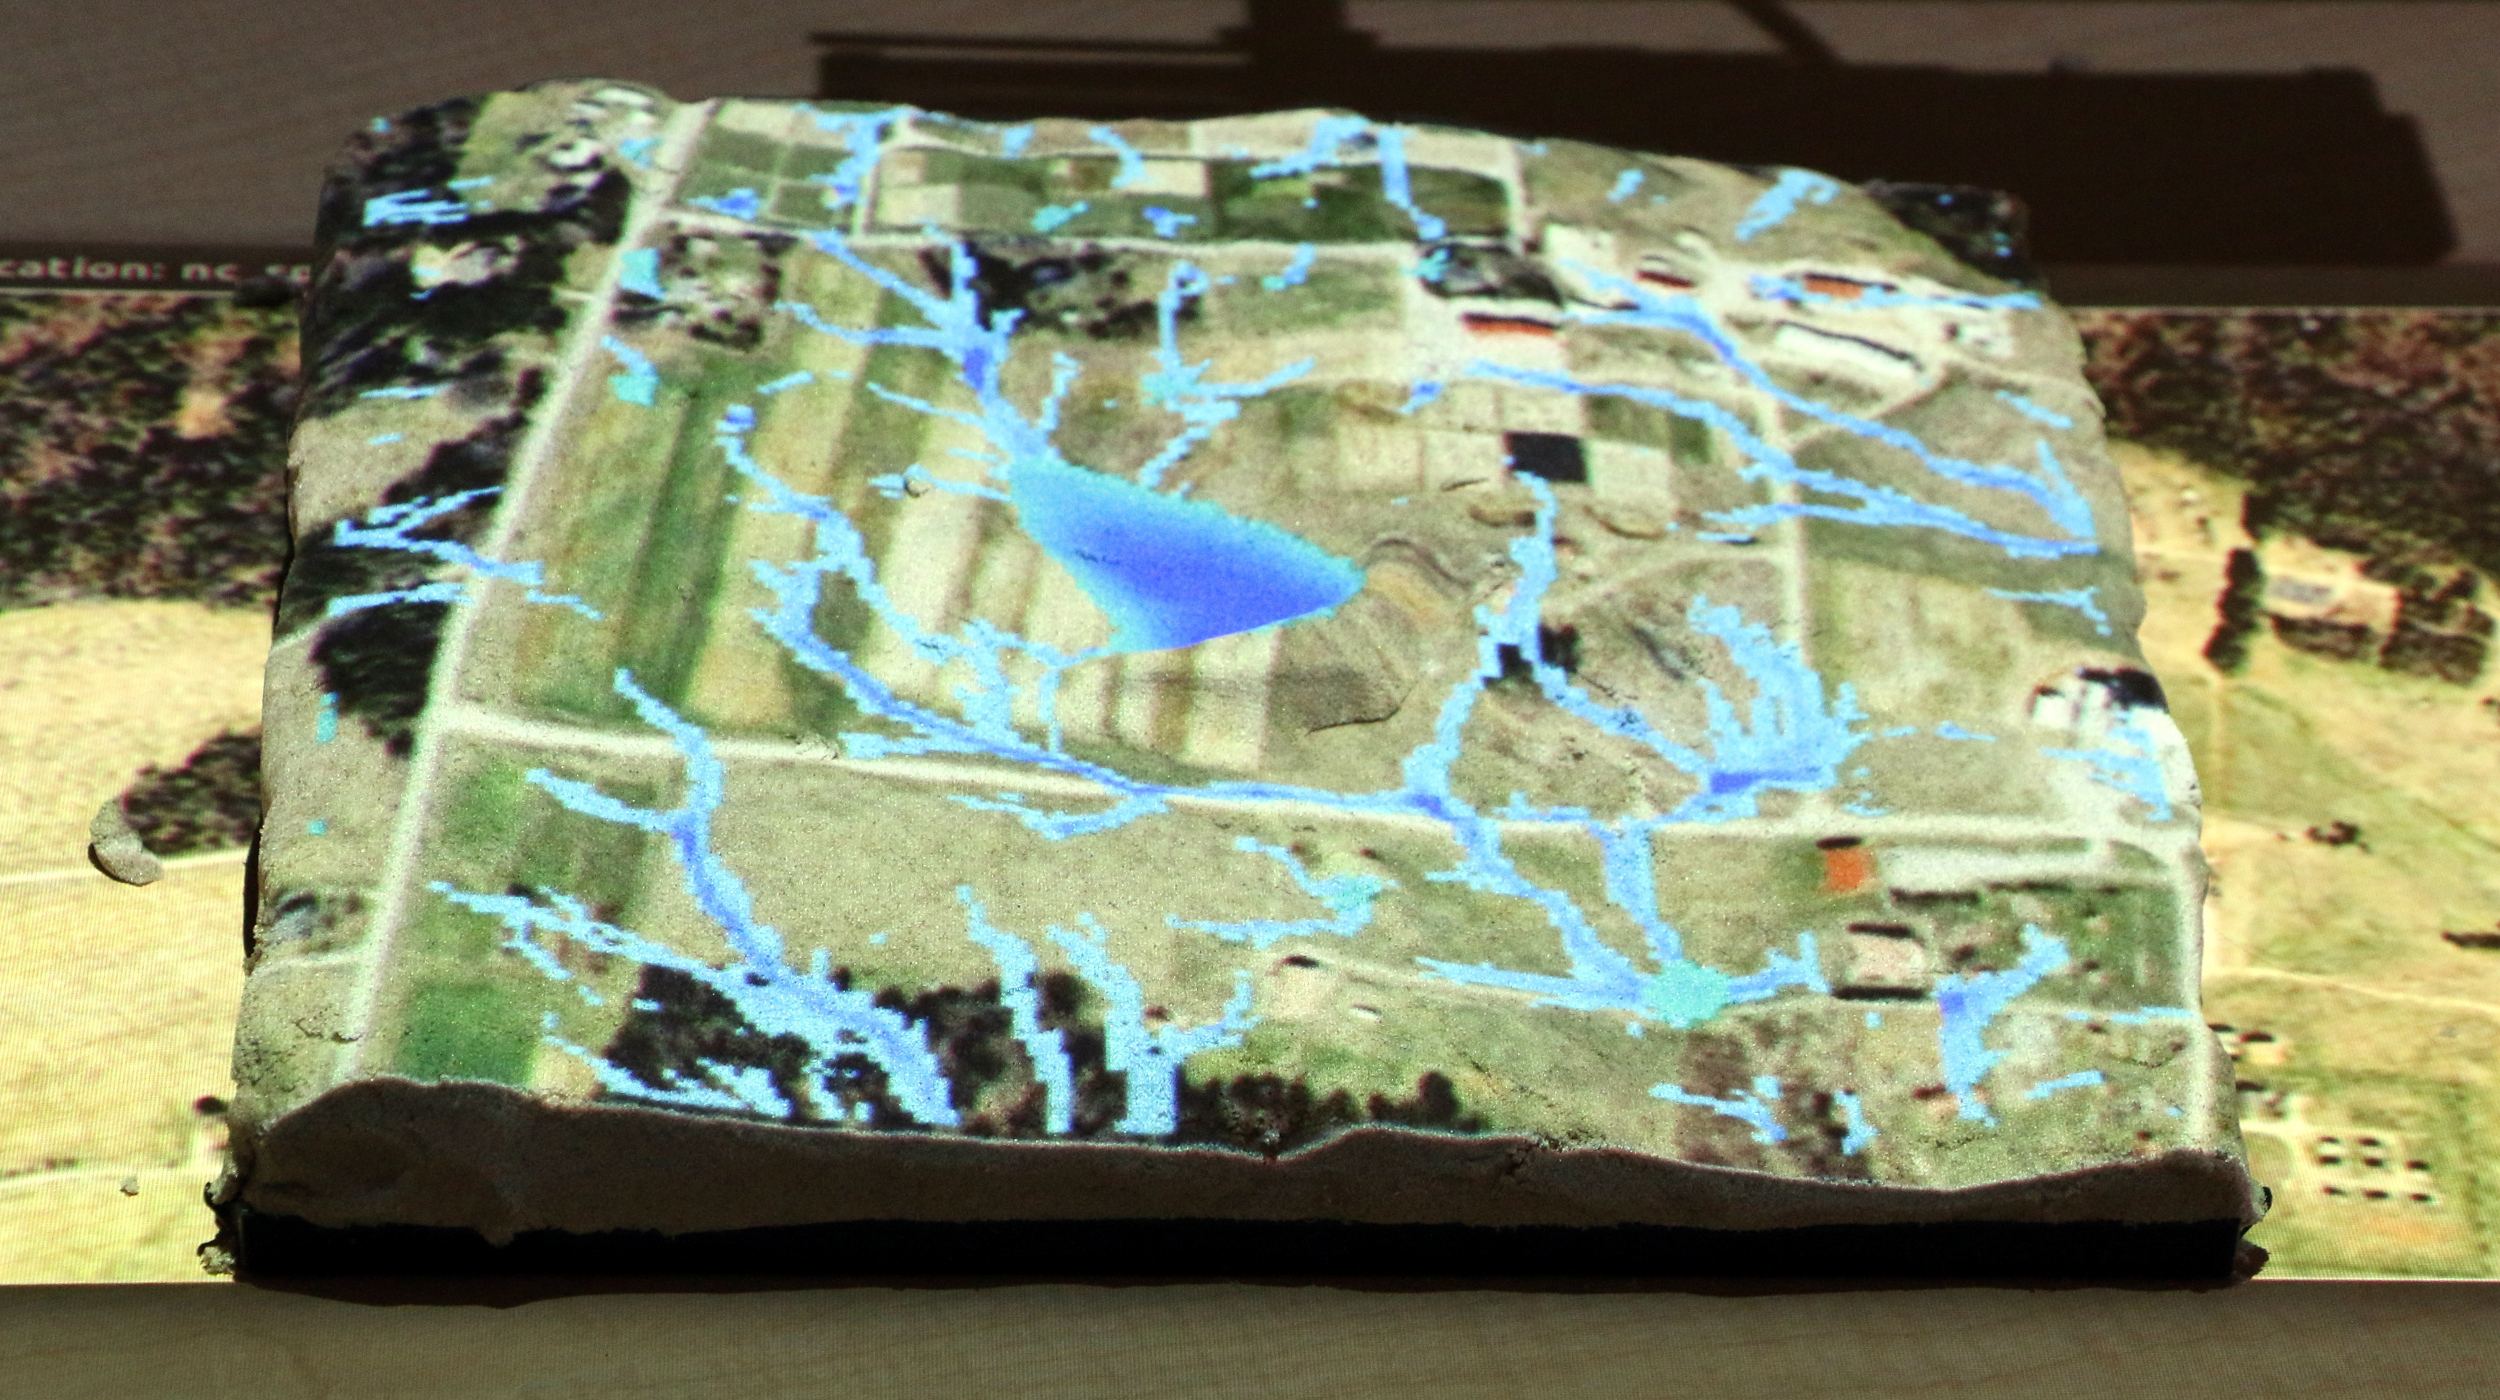
\includegraphics[width=0.49\textwidth]{images/applications/tl_sequence_3.jpg}
	\caption{Modeling the flow of water with Tangible Landscape. 
	A user sculpts a polymeric sand model of a landscape
	augmented with simulated water flow and an orthophotograph.  
	Changes to the model are scanned into in GIS 
	and the resulting water flow simulation is
	projected back onto the model in real-time.}
	\label{fig:tl_flow}
\end{center}
\end{figure}

Spatial thinking -- `the mental processes of representing, analyzing, and drawing inferences from spatial relations' \cite{Uttal2013} -- is used pervasively in everyday life for tasks such as recognizing things, manipulating things, interacting with others, and way-finding. 
% 
Higher dimensional spatial thinking 
-- thinking about form, volume, and processes unfolding in time -- 
plays an important role in 
science, technology, engineering, the arts, and math. 
%
3-dimensional (3D) spatial thinking is used in disciplines 
such as geology to understand the structure of the earth, 
ecology to understand the structure of ecosystems, 
civil engineering to shape landscapes, 
architecture to design buildings,
urban planning to model cities,
and the arts to shape sculpture.

Many spatial tasks can be performed computationally 
enabling users to efficiently store, model, and analyze large sets of spatial data 
and solve complex spatiotemporal problems.
%
In engineering, design, and the arts 
computer-aided design (CAD) and 3D modeling software are used 
to interactively, computationally model, analyze, and animate complex 3D forms.
%
In scientific computing
multidimensional spatial patterns and processes can be 
mathematically modeled, simulated, and optimized 
using geographic information systems (GIS), 
geospatial programming, and 
spatial statistics. 
%
GIS can be used to quantitatively model, analyze, simulate, and visualize 
complex spatial and temporal phenomena 
-- computationally enhancing users' understanding of space. 
%
With extensive libraries for point cloud processing, 
3D vector modeling, and
surface and volumetric modeling and analysis
GIS are powerful tools for studying 3D space.

GIS, however, can be unintuitive, challenging to use, and creatively constraining
due to the complexity of the software, 
the complex workflows, 
and the limited modes of interaction and visualization 
\cite{Ratti2004}. 
%
Unintuitive interactions with GIS can 
frustrate users,
constrain how they think about space, and add new cognitive burdens
that require highly developed spatial skills and reasoning to overcome. 
%
The paradigmatic modes for interacting with GIS today 
-- command line interfaces (CLI) and
graphical user interfaces (GUI) -- 
require physical input into devices like 
keyboards, mice, digitizing pens, and touch screens, 
but output data visually as text or graphics. 
%
Theoretically this disconnect between intention, action, and feedback 
makes graphical interaction unintuitive \cite{Dourish2001,Ishii2008}. 
%
Since users can only think about space visually with GUIs,
they need sophisticated spatial abilities 
like mental rotation \cite{Shepard1971,Just1985}
%spatial visualization, and spatial perception \cite{Linn1985}
to parse and understand, much less manipulate 
3D space. %in a GIS using a GUI. 

In order to make 3D GIS more natural and intuitive to use
we have designed Tangible Landscape 
-- a tangible interface for GIS --
that physically manifests 3D data 
so that users can feel and manipulate it with their bodies 
(Fig.~\ref{fig:tl_flow}). 
%
Our goal is for users with little or no computer experience 
to be able to intuitively, collaboratively explore 
%higher dimensional %multidimensional 
3D spatial data 
and interact with scientific models
so that they can 
rapidly test ideas while learning from computational feedback. 
%
We have begun to
quantitatively analyze how 
Tangible Landscape mediates 3D spatial cognition. 
%
We invite other researchers to collaborate 
in this ongoing open source and open science project 
by building Tangible Landscape,
contributing to its development,
developing new applications, 
and studying how it mediates cognition. 

\subsection{Tangible, embodied interaction}

In embodied cognition higher cognitive processes are 
grounded in, built upon, and mediated by bodily experiences 
such as kinaesthetic perception and action \cite{Hardy-Vallee2008}. 
%
Tangible interfaces 
-- interfaces that couple physical and digital data \cite{Dourish2001} -- 
are designed to enable embodied interaction
by physically manifesting digital data 
so that users can cognitively grasp and absorb it,
thinking with it rather than about it \cite{Kirsh2013}. 
%
Embodied interaction should be highly intuitive --
drawing on existing motor schemas
and seamlessly connecting intention, action, and feedback.
%
It should reduce users' cognitive load 
by enabling them to
physically simulate processes 
and offload tasks like 
spatial perception and manipulation onto the body
\cite{Kirsh2013}.
%
%Users should be able to 
%subconsciously, kinaesethically judge and manipulate 
%spatial distances, relationships, patterns, 3D forms, and volumes
%offloading these challenging cognitive tasks onto their bodies.
%
Distance and physical properties 
like size, shape, volume, weight, hardness, and texture
can be automatically and subconsciously assessed 
with the body \cite{Jeannerod1997}.
Tangible interfaces should, therefore, enable users to
subconsciously, kinaesethically judge and manipulate 
spatial distances, relationships, patterns, 3D forms, and volumes
offloading these challenging cognitive tasks onto their bodies.

\subsection{Tangible interfaces for geospatial modeling} 

% ---------------------------- REVISIONS ---------------------------- 
% 
% Detailed discussion of related work
% 	Compare similar systems to TL
% 	Evaluate other systems
% 		See TL book
% 	Discuss relevant user studies
% 
% -------------------------------------------------------------------------- 

% EDITOR: Provide more details in related work section that differentiates your work/findings from related work.

% REFEREE 1: The paper presents a sizeable number of recently published papers on related work. Unfortunately, most papers are only enumerated in four tables, focusing on different aspects. For a journal article, a more detailed discussion would be appropriate. In particular, it is not clear how these systems compare to the Tangible Landscape system. Even though the focus of this submitted paper is on the evaluation of the system rather than the system itself, readers should to be able to understand the relevance of the evaluations for other systems. Furthermore, a few prior evaluations of tangible interfaces for geospatial modeling are cited, but not discussed either. What were the results/conclusions of such prior evaluations?

% REFEREE 2: 
% The studies by Woods (Woods 2016) and Schmidt-Daly (Schmidt-Daly 2016) may have been too recent at the time of submission, but they are highly relevant related work on how augmented sand interfaces for GIS are used as teaching tools and to investigate spatial knowledge.
% The appeal of the contribution could be broadened by providing examples of similar systems for other application domains, such as volumetric data exploration (Ratti 2003) and music (Kikukawa 2013), gaming (Wilson 2007), and animation (Kazi 2011).
% While not a continuous sand TUI, GeoTUI, as a study of a tangible user interface for GIS experts should be mentioned as well (Couture 2008).

% REFERENCES
%Nadine Couture, Guillaume Rivière, and Patrick Reuter. 2008. GeoTUI: a tangible user interface for geoscience. In Proceedings of the 2nd international conference on Tangible and embedded interaction (TEI '08). ACM, New York, NY, USA, 89-96. DOI=http://dx.doi.org/10.1145/1347390.1347411
%
%Kazi, Rubaiat Habib, et al. "SandCanvas: a multi-touch art medium inspired by sand animation." Proceedings of the SIGCHI Conference on Human Factors in Computing Systems. ACM, 2011.
%
%Kikukawa, Yuya, et al. "Hakoniwa: A sonification art installation consists of sand and woodblocks." (2013).
%
%Ratti, Carlo, et al. "PHOXEL-SPACE: an interface for exploring volumetric data with physical voxels." Proceedings of the 5th conference on Designing interactive systems: processes, practices, methods, and techniques. ACM, 2004.
%
%Tarah N. Schmidt-Daly, Jennifer M. Riley, Charles R. Amburn, Kelly S. Hale, and P. David Yacht
%Video Game Play and Effect on Spatial Knowledge Tasks Using an Augmented Sand Table Proceedings of the Human Factors and Ergonomics Society Annual MeetingSeptember 2016 60: 1429-1433, doi:10.1177/1541931213601328
%
%Wilson, A. Depth-Sensing Video Cameras for 3D Tangible Tabletop Interaction, Tabletop 2007.
%
%Woods, Terri L., et al. "Pilot Study Using the Augmented Reality Sandbox to Teach Topographic Maps and Surficial Processes in Introductory Geology Labs." Journal of Geoscience Education 64.3 (2016): 199-214.


With GIS users can computationally offload complex cognitive tasks 
like analyzing spatial patterns and simulating spatiotemporal processes.
%
Tangible interfaces for geospatial modeling should, 
therefore, enhance users' spatial performance 
-- their ability to sense, manipulate, and interact with multidimensional space -- 
for challenging tasks 
like sculpting topography and guiding the flow of water
by combining these physical and computational affordances.
%
There are already many tangible interfaces for geospatial modeling.
%
%Tangible interfaces for geospatial modeling 
These include 
augmented architectural models (Table~\ref{table:review_a}), 
augmented clay (Table~\ref{table:review_b}),  
augmented sandboxes (Table~\ref{table:review_c}), 
and actuated pin tables (Table~\ref{table:review_d}).

Projection-augmented tangible interfaces 
couple a physical and digital model
through a cycle of 3D sensing or object recognition,
computation, and projection. 
%
Augmented architectural models
like Urp \cite{Underkoffler1999} 
and the Collaborative Design Platform \cite{Schubert2011}
are a type of 
`discrete tabletop tangible interface' \cite{Ishii2012}
with physical models of buildings 
that are augmented with projected analytics.
%
Augmented clay models 
like Illuminating Clay \cite{Piper2002a} 
and augmented sandboxes like Sandscape \cite{Ishii2004} 
are types of 
`deformable, continuous tangible interfaces' \cite{Ishii2012}
that users can sculpt. 
%
These tangible interfaces 
have two feedback loops -- 
there is passive, kinaesthetic feedback from grasping the physical model 
and active, graphical feedback from computation.

Actuated pin tables
like Relief \cite{Leithinger2009}
are a type of transformable tangible interface \cite{Ishii2012} 
or shape changing interface \cite{Rasmussen2012}
that can physically change shape based on computation.
%which use `physical change of shape as input or output' \cite{Rasmussen2012}. 
%
These tangible interfaces 
have a third feedback loop --
the physical model
can be computationally transformed
for active, kinaesthetic feedback. 

Research on tangible interfaces for geospatial modeling 
has focused on the design of new technologies and prototypes
rather than studying how they
are used. 
%
A review of tangible interfaces for geospatial modeling 
(Tables~\ref{table:review_a}-\ref{table:review_d})
shows that there have been 
relatively few case studies \cite{Ishii2002,Tateosian2010,Petrasova2015} 
or qualitative user studies \cite{Shamonsky2003}
and only a single quantitive pilot study \cite{Harmon2016}.
%
A review of shape-changing interfaces 
also found that there were relatively few user studies
and called for `more, high-quality data on user experience'
in order to understand if interfaces work as designed
\cite{Rasmussen2012}.

% RESEARCH QUESTIONS

% ---------------------------- REVISIONS ---------------------------- 
% 
% Novice vs. expert systems
% 	What functionality is needed for expert modeling tasks?
% 
% -------------------------------------------------------------------------- 

% REFEREE 2: 
% This article presents a study of how tangible user interfaces can aid spatial modeling tasks. “Tangible Landscape” is the culmination of years of research, which have been published in articles and books, and the contribution of this article over such prior work is a study to compare the system to a graphical user interface for 3D modeling, and to investigate the effect of projected feedback. The results are interesting: study participants produce more detailed and defined models with this projection-augmented tangible interface. While the study tasks are domain-specific to GIS, its contribution is relevant for the wider HCI community: Various tangible user interfaces for 3D modeling have been proposed in the past, but only few studies exist to quantify how well they perform compared to graphical user interfaces. The sandbox form factor is well suited for such a comparison, as it has recently gained traction and public interest with versions of the UC Davis “AR Sandbox” being installed in many locations (see https://arsandbox.ucdavis.edu/#mapid), targeting mainly introductory classroom exercises and public science museums. In contrast, this “Tangible Landscape” system and study is designed for domain experts. I believe that TOCHI readers will be interested in the implications whether such TUI modeling systems can be suitable not only for novice users, but also for use by experts, and what functionality can support such modeling tasks.

Many of the theoretical underpinnings of tangibles 
remain unproven and unexplored. 
Do current approaches to tangible, embodied interfaces
really work as theorized? 
Can users successfully
cognitively grasp digital data as an extension of their bodies,
intuitively interact, 
and offload cognitive processes
with tangibles?
How does this change how users think and perform?
How does it mediate spatial cognition and performance? 
Can tangible interfaces for geospatial modeling 
enhance spatial thinking
through kinaesthetic interaction with 
spatial computations?
Can users offload enough cognitive work onto their bodies
to successfully parse and learn from computational feedback
without suffering cognitive overload?

In order to begin to answer some of these questions we 
designed a tangible interface for geospatial modeling, 
while simultaneously conducting an experiment
to study how this tangible interface mediates spatial cognition.
%
Our research objectives were to:
%
\begin{itemize}
\item Design an effective tangible interface for geospatial modeling
\item Test whether coupling a physical and digital model of topography can improve 3D spatial performance
\item Study how different geospatial analytics mediate users' 3D spatial performance when using a tangible interface for geospatial modeling
\end{itemize}


\begin{table}
\tbl{Augmented architectural modeling interfaces}{
\ra{1.5}
\begin{tabulary}{1.0\textwidth}{LLCLL}
\toprule
System & \mbox{Interaction} & GIS & User studies & Publications\\
\midrule
%
Urp & Object detection && \mbox{Case studies\textsuperscript{\textasteriskcentered}} & \cite{Underkoffler1999}\\
&&&& \cite{Ishii2002}\textsuperscript{\textasteriskcentered}\\
%
Collaborative Design Platform & Object detection &&& \cite{Schubert2011}\\
& Touch &&& \cite{Schubert2011a}\\
& Sketching &&&  \cite{Schubert2012}\\
&&&& \cite{Schubert2014}\\
&&&& \cite{Schubert2015}\\
%&&&& \cite{Schubert2013}\\
%&&&& \cite{Schubert2014a}\\
%
\bottomrule
\end{tabulary}}
\label{table:review_a} 
%
\vspace*{1.5em}
%
\tbl{Augmented clay interfaces}{
\ra{1.5}
\begin{tabulary}{1.0\textwidth}{LLLCLL}
\toprule
System & \mbox{Interaction} & GIS & User studies & Publications\\
\midrule
%
Illuminating Clay & Sculpting && Protocol analysis\textsuperscript{\textdaggerdbl} & \cite{Piper2002a}\\
&&&& \cite{Piper2002b}\\
&&&& \cite{fielding-piper2002}\\
&&&& \cite{Shamonsky2003}\textsuperscript{\textdaggerdbl}\\
&&&& \cite{Ishii2004}\\
&&&& \cite{Ratti2004}\\
%
Tangible Geospatial Modeling System & Sculpting & \cmark & Case studies\textsuperscript{\textasteriskcentered} & \cite{Mitasova2006}\\
&&&& \cite{Tateosian2010}\textsuperscript{\textasteriskcentered}\\
%
\bottomrule
\end{tabulary}}
\label{table:review_b} 
%
\vspace*{1.5em}
%
\tbl{Augmented sandbox interfaces}{
\ra{1.5}
\begin{tabulary}{1.0\textwidth}{LLLCLL}
\toprule
System & \mbox{Interaction} & GIS & User studies & Publications\\
\midrule
%
SandScape& Sculpting &&& \cite{Ishii2004}\\
&&&& \cite{Ratti2004}\\
%
SandyStation & Sculpting &&&\\ 
%
Augmented Reality Sandbox & Sculpting &&& \cite{Reed2014}\\
& Gesture\\
%
Rapid Landscape Prototyping Machine & Machining &&& \cite{Robinson2014}\\
%
Tangible Landscape & Sculpting & \cmark & Case studies\textsuperscript{\textasteriskcentered} & \cite{Petrasova2014}\\
& Object detection && Quantitative experiments\textsuperscript{\textdagger} & \cite{Petrasova2015}\textsuperscript{\textasteriskcentered}\\
& Sketching &&& \cite{Harmon2016}\textsuperscript{\textdagger}\\
%&&&& \cite{Harmon2016a}\\
%
The Augmented REality Sandtable (ARES) & Sculpting &&& \cite{Amburn2015}\\
& Gesture\\
%
\bottomrule
\end{tabulary}}
\label{table:review_c} 
\end{table}
%
\begin{table}
\tbl{Actuated pin table interfaces}{
\ra{1.5}
\begin{tabulary}{1.0\textwidth}{LLCLL}
\toprule
System & \mbox{Interaction} & GIS & User studies & Publications\\
\midrule
%
XenoVision Mark III Dynamic Sand Table & Sculpting &&&\\
%
Northrop Grumman Terrain Table & Sculpting &&&\\
%
Relief & Sculpting &&& \cite{Leithinger2009}\\
&&&& \cite{Leithinger2010}\\
%
Recompose & Sculpting &&& \cite{Leithinger2011}\\
& Gesture &&& \cite{Blackshaw2011}\\
%
Tangible CityScape & Gesture &&&\\
% 
Inform & Sculpting &&& \cite{Follmer2013}\\
& Gesture\\
& Object detection\\
%
\bottomrule
\end{tabulary}}
\label{table:review_d} 
\end{table}

\section{Tangible Landscape}

\subsection{Concept}

% ---------------------------- REVISIONS ---------------------------- 
% 
% Frame as an expert system
% 	vs. AR Sandbox as novice system
%
% Maps
% 	Add map of TL?
% 	Add map of AR Sandbox?
% 
% -------------------------------------------------------------------------- 

% REFEREE 2: 
% ...Various tangible user interfaces for 3D modeling have been proposed in the past, but only few studies exist to quantify how well they perform compared to graphical user interfaces. The sandbox form factor is well suited for such a comparison, as it has recently gained traction and public interest with versions of the UC Davis “AR Sandbox” being installed in many locations (see https://arsandbox.ucdavis.edu/#mapid), targeting mainly introductory classroom exercises and public science museums. In contrast, this “Tangible Landscape” system and study is designed for domain experts. I believe that TOCHI readers will be interested in the implications whether such TUI modeling systems can be suitable not only for novice users, but also for use by experts, and what functionality can support such modeling tasks.

Tangible interfaces for GIS 
should ease the cognitive burden of 
visualizing, interacting with, 
and reasoning about space
by giving spatial data an interactive, physical form 
that users can cognitively grasp and kinaesthetically explore. 
%
Tangible Landscape -- a tangible user interface for GRASS GIS --
couples a physical and digital model of a landscape through a continuous cycle of 3D scanning, geospatial modeling, and projection
so that users can intuitively interact with the modeled landscape in real-time.
%
Conceptually Tangible Landscape physically manifests 3D data 
so that users can hold a GIS in their hands -- 
so that they can, for example, feel the shape of the earth, sculpt its topography, and direct the flow of water with their hands.
%
It enables users to 3D sketch -- 
to naturally model forms such as topography, 
draw points and polygons, 
and interact with simulated physical processes -- 
in a rapid, iterative process 
of observation, hypothesis generation and testing, and inference. 
%
Tangible Landscape is meant to fluidly, seamlessly combine
computational science with exploratory modes of creative thinking.

Tangible Landscape is unique because it is the only 
real-time tangible interface for spatial modeling that 
\begin{enumerate*}
\item is powered by a GIS,
\item has extensive libraries for rasters, vectors, time-series, statistics, modeling, analysis, simulation, visualization, and databasing, 
\item physically represents space with enough precision for real-world problem solving,
\item has been demonstrated for a wide range of applications,
\item and has been quantitatively tested in user experiments. 
\end{enumerate*}

\subsection{Evolution}
Tangible Landscape evolved from 
Illuminating Clay \cite{Piper2002a} and 
the Tangible Geospatial Modeling System (TanGeoMS) \cite{Tateosian2010}. 
% Illuminating Clay
Illuminating Clay coupled a clay model and digital model of landscape 
through a cycle of laser scanning, spatial modeling, and projection.
By enriching physical models of urban spaces and landscapes 
with spatial analyses  
such as 
elevation, aspect, slope, cast shadow, profile, curvature, 
viewsheds, solar irradiation, and water direction
it enabled
intuitive form-finding, 
streamlined analog and digital workflows, 
and enabled multiple users to simultaneously interact in a natural way \cite{Ratti2004}. 
Illuminating Clay had a very limited library of custom implemented spatial analyses. 
Since many of analyses were adapted 
from the open source GRASS GIS project \cite{Piper2002a} 
there was a call for closer integration with GRASS GIS 
in order to draw on its extensive libraries 
for spatial computation \cite{Piper2002b}. 
The effort to couple a physical landscape model with GRASS GIS \cite{Mitasova2006} 
led to the development of 
TanGeoMS \cite{Tateosian2010}.

% Tangible Geospatial Modeling System
TanGeoMS coupled a physical model and GIS model of a landscape 
through a cycle of laser scanning, 
geospatial computation in GRASS GIS, and projection
giving developers and users access to 
a sophisticated library for 
spatial modeling, simulation, visualization, and databasing.
It enriched freeform hand modeling with geospatial simulations 
like diffusive water flow and erosion-deposition 
so that users could easily explore how 
changes in topographic form affect landscape processes. 

% Augmented Reality Sandbox
Tangible Landscape -- the next generation of this system -- was inspired by
the open source Augmented Reality Sandbox \cite{Kreylos2012}
which couples a sandbox with a digital model of a landscape 
through a real-time cycle of 3D scanning with a Kinect sensor, spatial modeling and simulation, and projection.
% TL
While TanGeoMS used an expensive laser scanner
for 3D sensing \cite{Tateosian2010}, 
Tangible Landscape uses a low-cost 3D sensor %like the Kinect 
for real-time depth and color sensing. 
The \nth{1} generation of Tangible Landscape \cite{Petrasova2014} 
used the \nth{1} generation Kinect with structured light sensing \cite{Smisek2011}, 
while the \nth{2}  \cite{Petrasova2015} and \nth{3} generations of Tangible Landscape 
used the \nth{2} generation Kinect with time-of-flight sensing \cite{Bamji2015}. 


\subsection{Design}

\begin{figure}
\begin{center}
		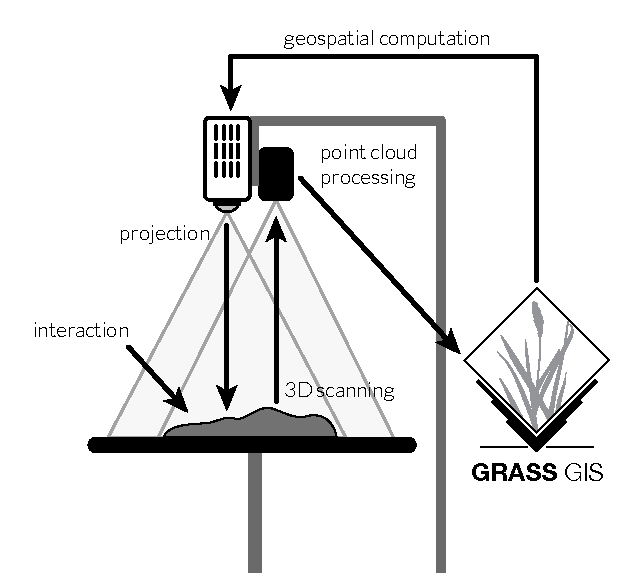
\includegraphics{images/system_schema.pdf}
	\caption{How Tangible Landscape works: a real-time feedback cycle of physical interaction, 3D scanning, point cloud processing, geospatial computation, and projection.}
	\label{fig:system_schema}
\end{center}
\end{figure}

\begin{figure}
\begin{center}
		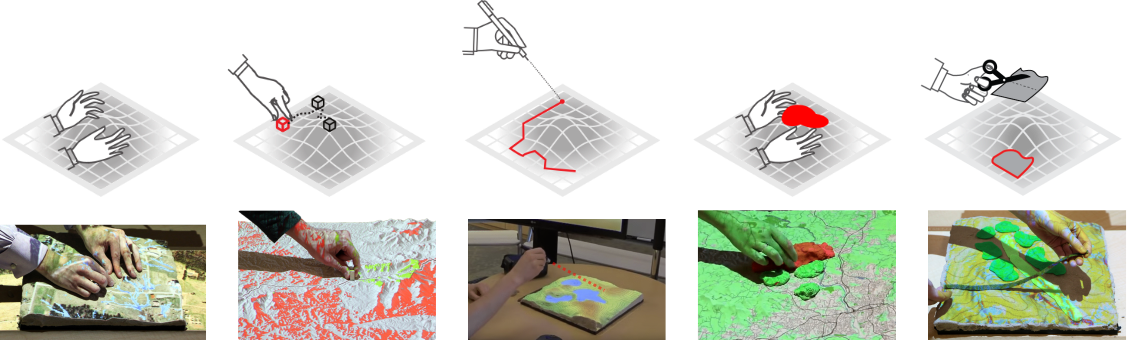
\includegraphics[width=\textwidth]{images/interactions.png}
	\caption{Modes of interaction with Tangible Landscape: sculpting surfaces, placing points, drawing lines, building volumes, and marking areas.}
	\label{fig:interactions}
\end{center}
\end{figure}

Tangible Landscape was designed to let users naturally explore 
spatial data, models, and simulations in an engaging, playful way
by 3D sketching (Fig.~\ref{fig:subsurface}). 
Users can work collaboratively, 
simultaneously interacting with the physical model
(Table \ref{table:tl_vr}) \cite{Tabrizian2016}. 
%(Fig.~\ref{fig:collaboration}). 
As users change the physical model
the model is 3D scanned as a point cloud, georeferenced, imported into GIS, 
and either binned or interpolated as a digital elevation model. 
The digital elevation model is used to compute 
geospatial analyses, models, and simulations, 
which are then projected back onto the physical model 
-- all in real-time (Fig.~\ref{fig:system_schema}). 
Users can tangibly interact with digital models and simulations
by sculpting, placing objects, or sketching (Fig.~\ref{fig:interactions}) .
They can sculpt the model with their hands
to shape topography, 
create or move volumes
like buildings or forest canopy, 
or explore 3D raster data.  
They can place objects or markers 
that will be identified using object and color recognition
in order to draw points, polylines, polygons, or volumes. 
They can also use a laser pointer to draw polylines or polygons
that will be detected based on light intensity. 
%(Fig.~\ref{fig:drawing_trees}). 
As the digital models and simulations update
the results are projected back onto the model for users to see. 
The results can also be rendered in 3D 
on a screen or head-mounted display like an Oculus Rift
so that users can immersively visualize the modeled landscape 
at a human scale 
(Table \ref{table:tl_vr}) \cite{Tabrizian2016}.
%(Fig.~\ref{fig:drawing_trees}).

Because the model is continually scanned
users' hands will be digitized as they sculpt or place objects. 
Scanning users' hands as topography 
%can be distracting; it also, however, 
helps users understand how the system works
%-- by seeing how direct interaction is --
and encourages play. 
Users can, for example, 
place their hands on the model and create simulated lakes between their fingers
(Fig.~\ref{fig:hands}) \cite{ncsu_geoforall_2016b}. 

\begin{figure}
\begin{center}
		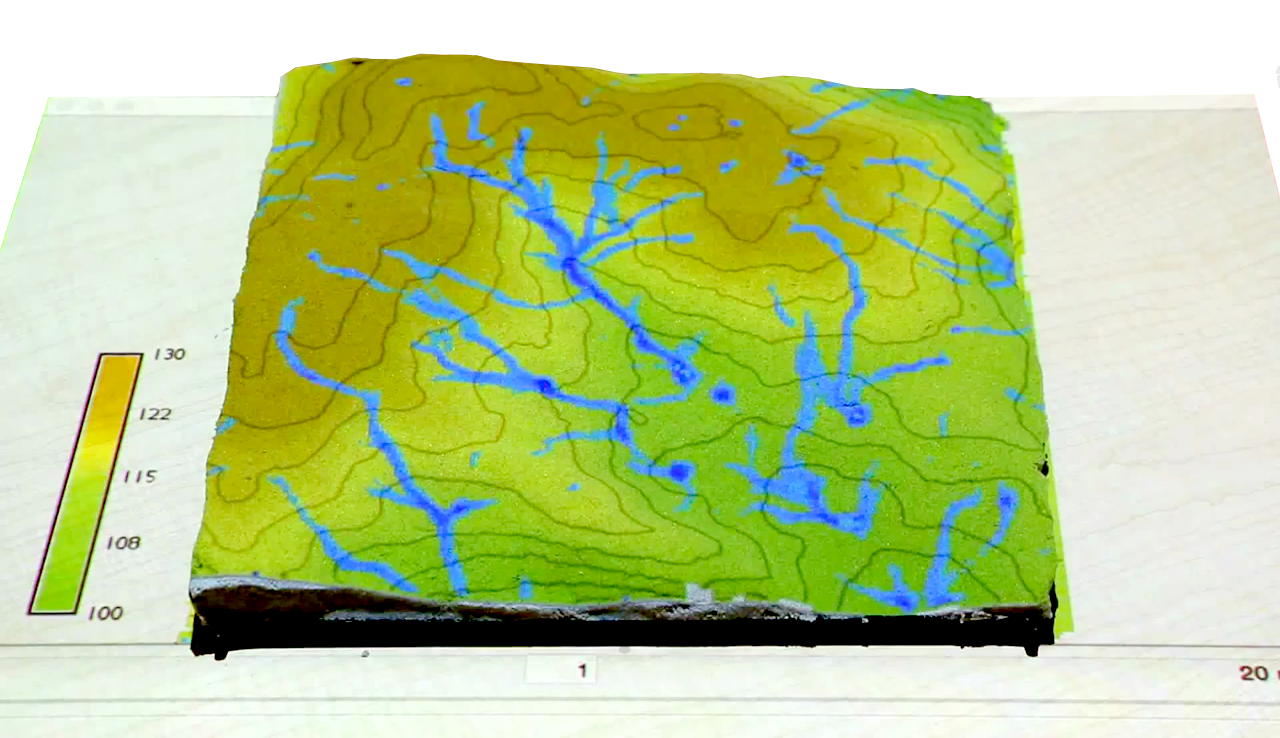
\includegraphics[width=0.32\textwidth]{images/hands/tl_hand_1.png}
		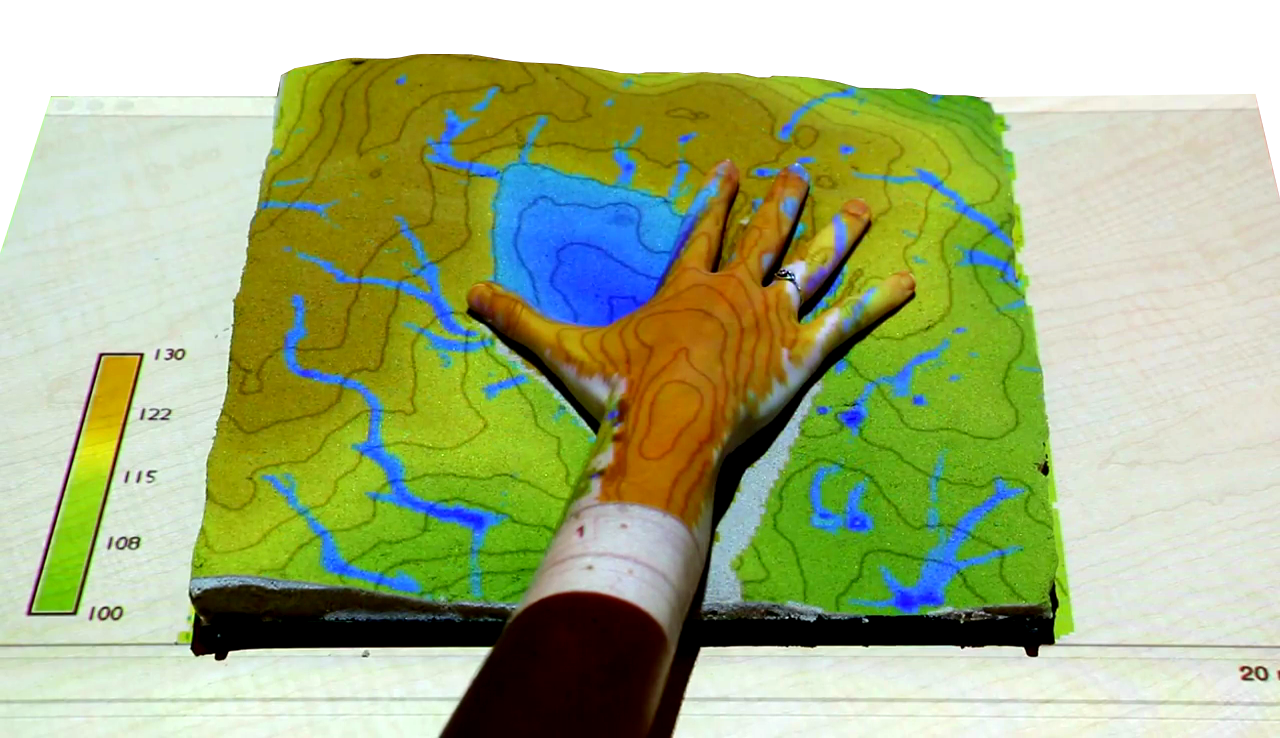
\includegraphics[width=0.32\textwidth]{images/hands/tl_hand_2.png}
		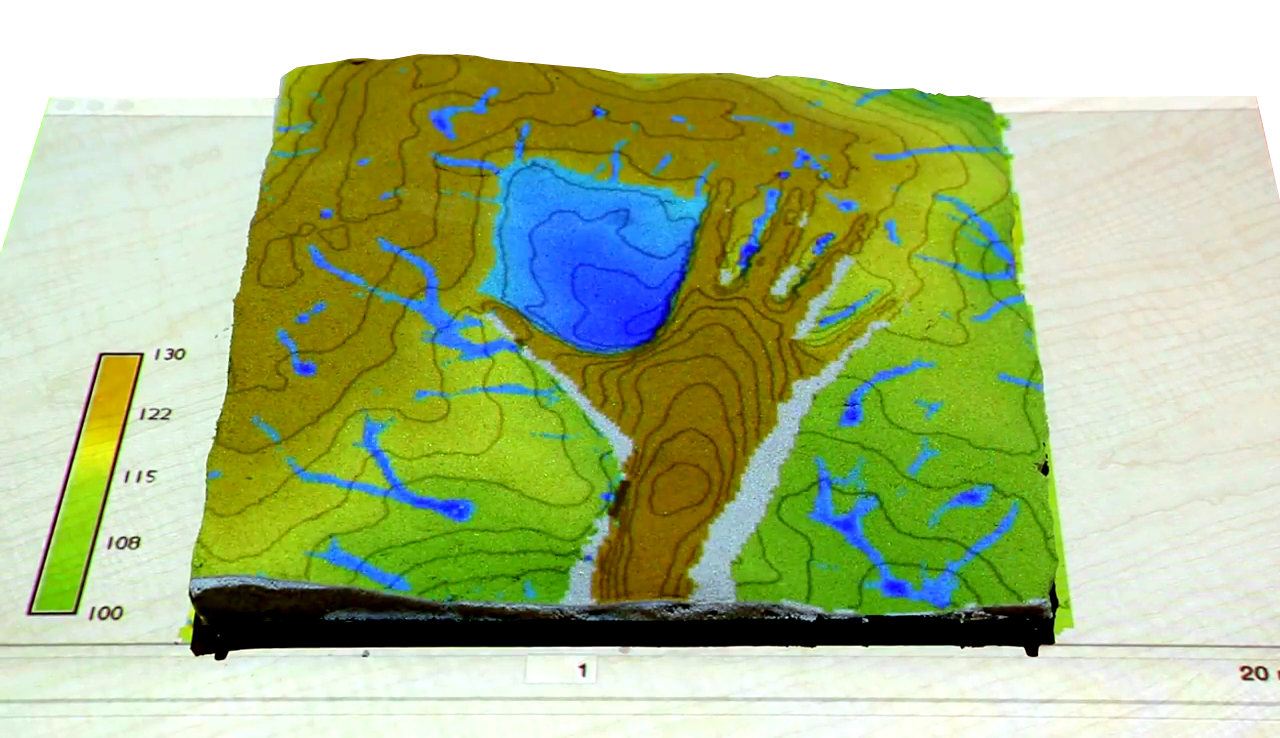
\includegraphics[width=0.32\textwidth]{images/hands/tl_hand_3.png}
	\caption{With Tangible Landscape users can scan their arms and hands as topography creating lakes between their fingers.}
	\label{fig:hands}
\end{center}
\end{figure}

\begin{figure}
\begin{center}
		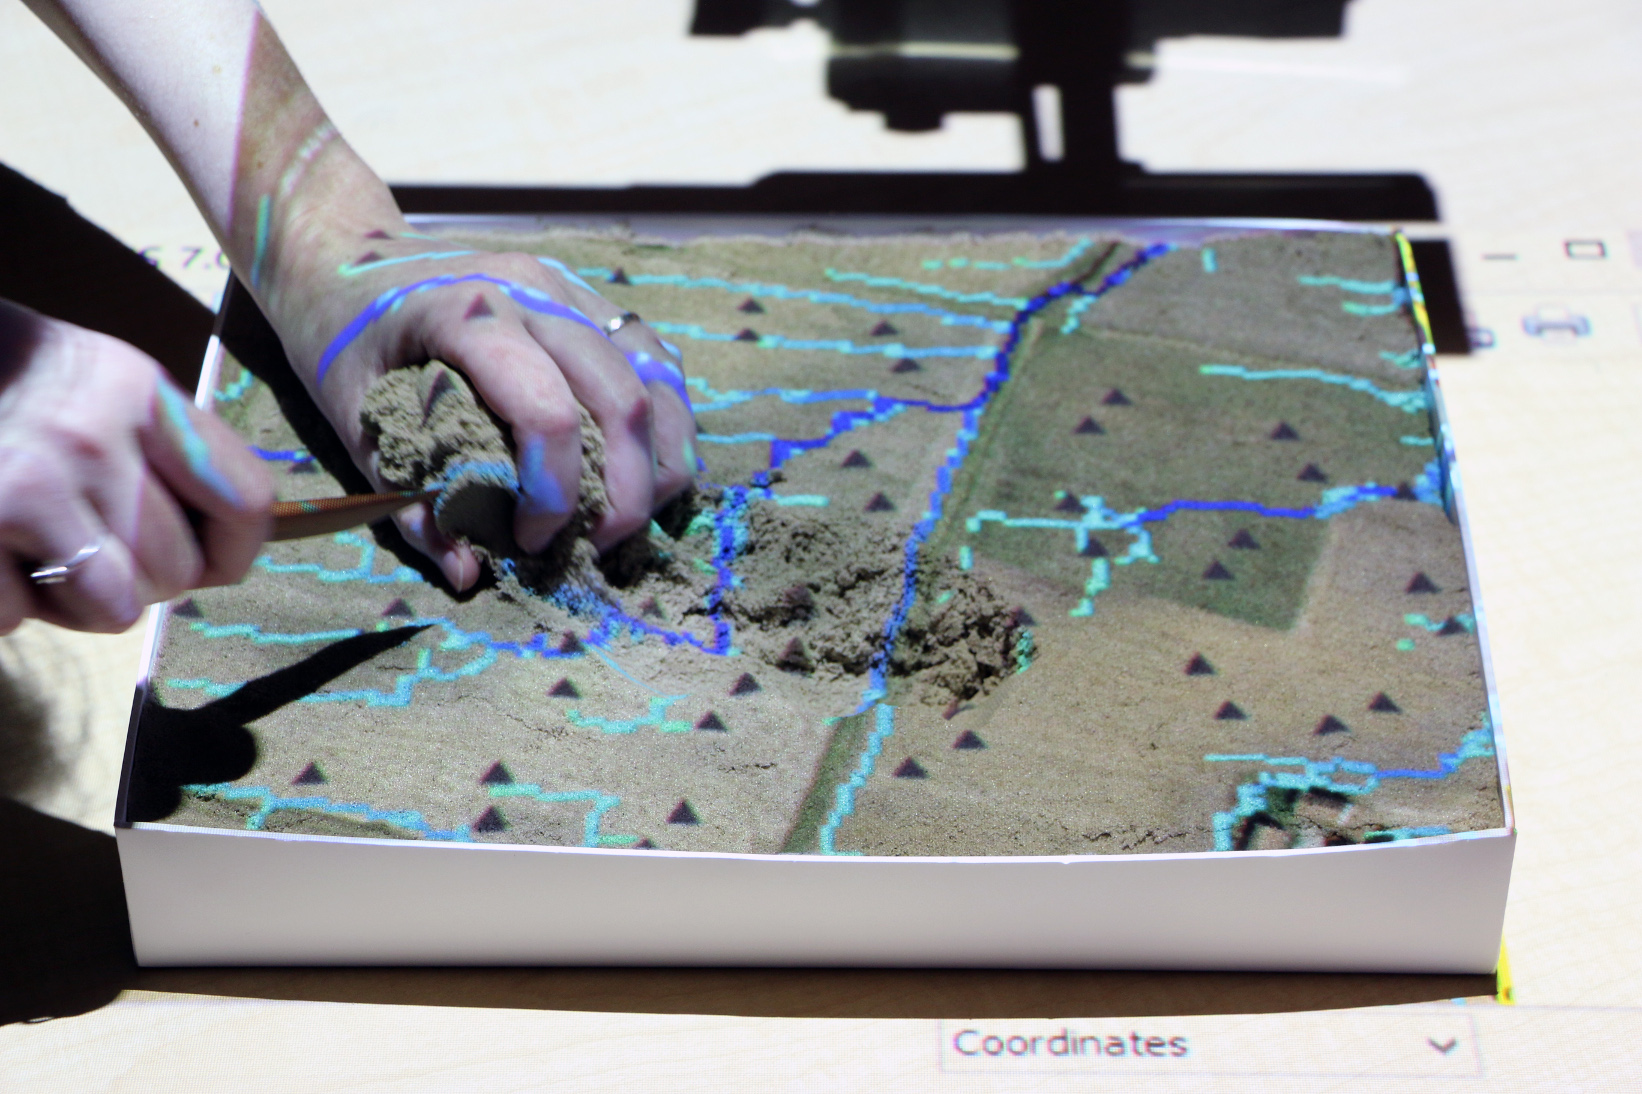
\includegraphics[height=70px]{images/applications/subsurface_1.jpg}
		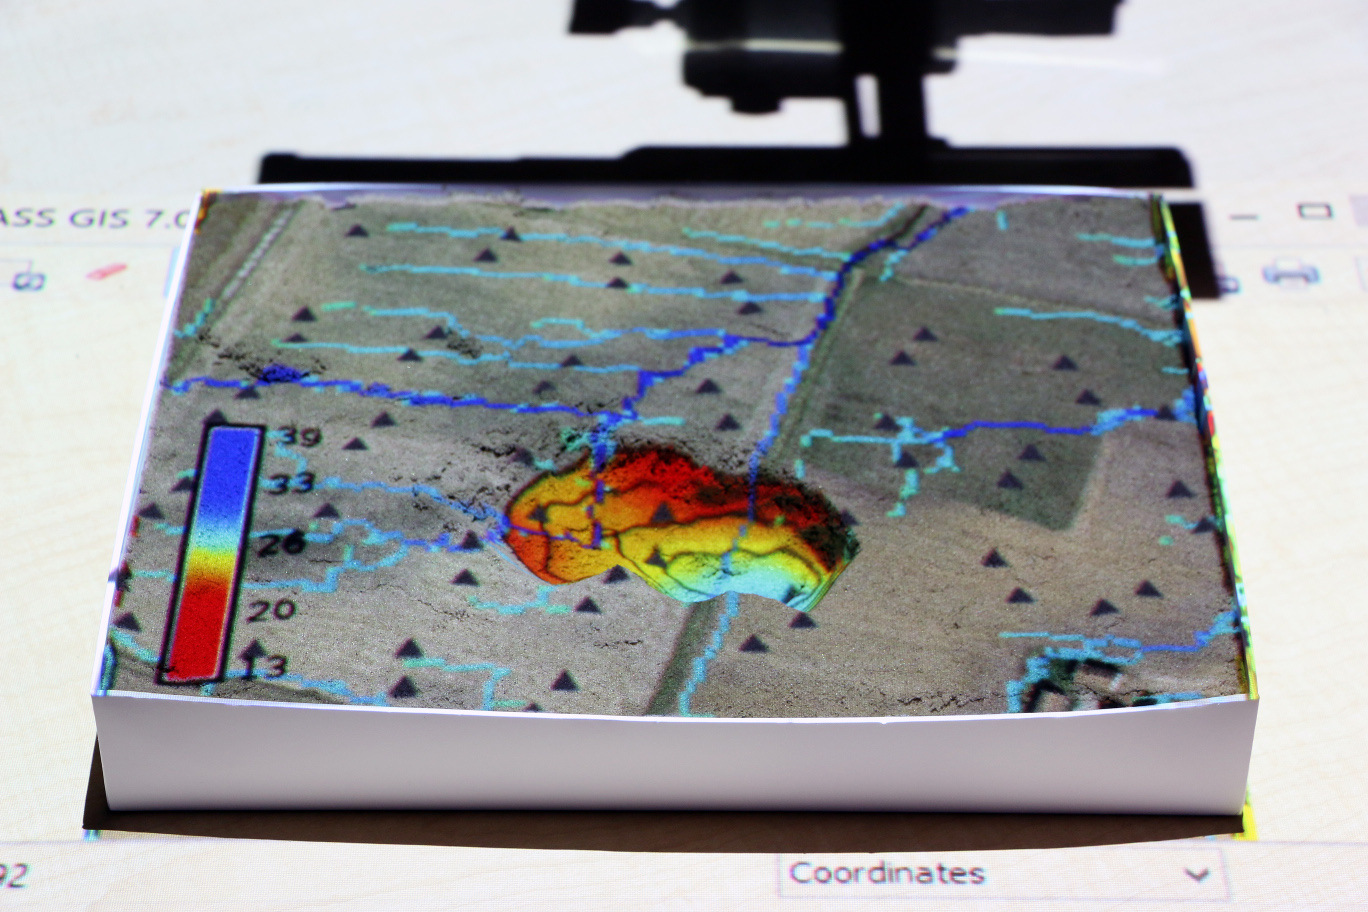
\includegraphics[height=70px]{images/applications/subsurface_2.jpg}
		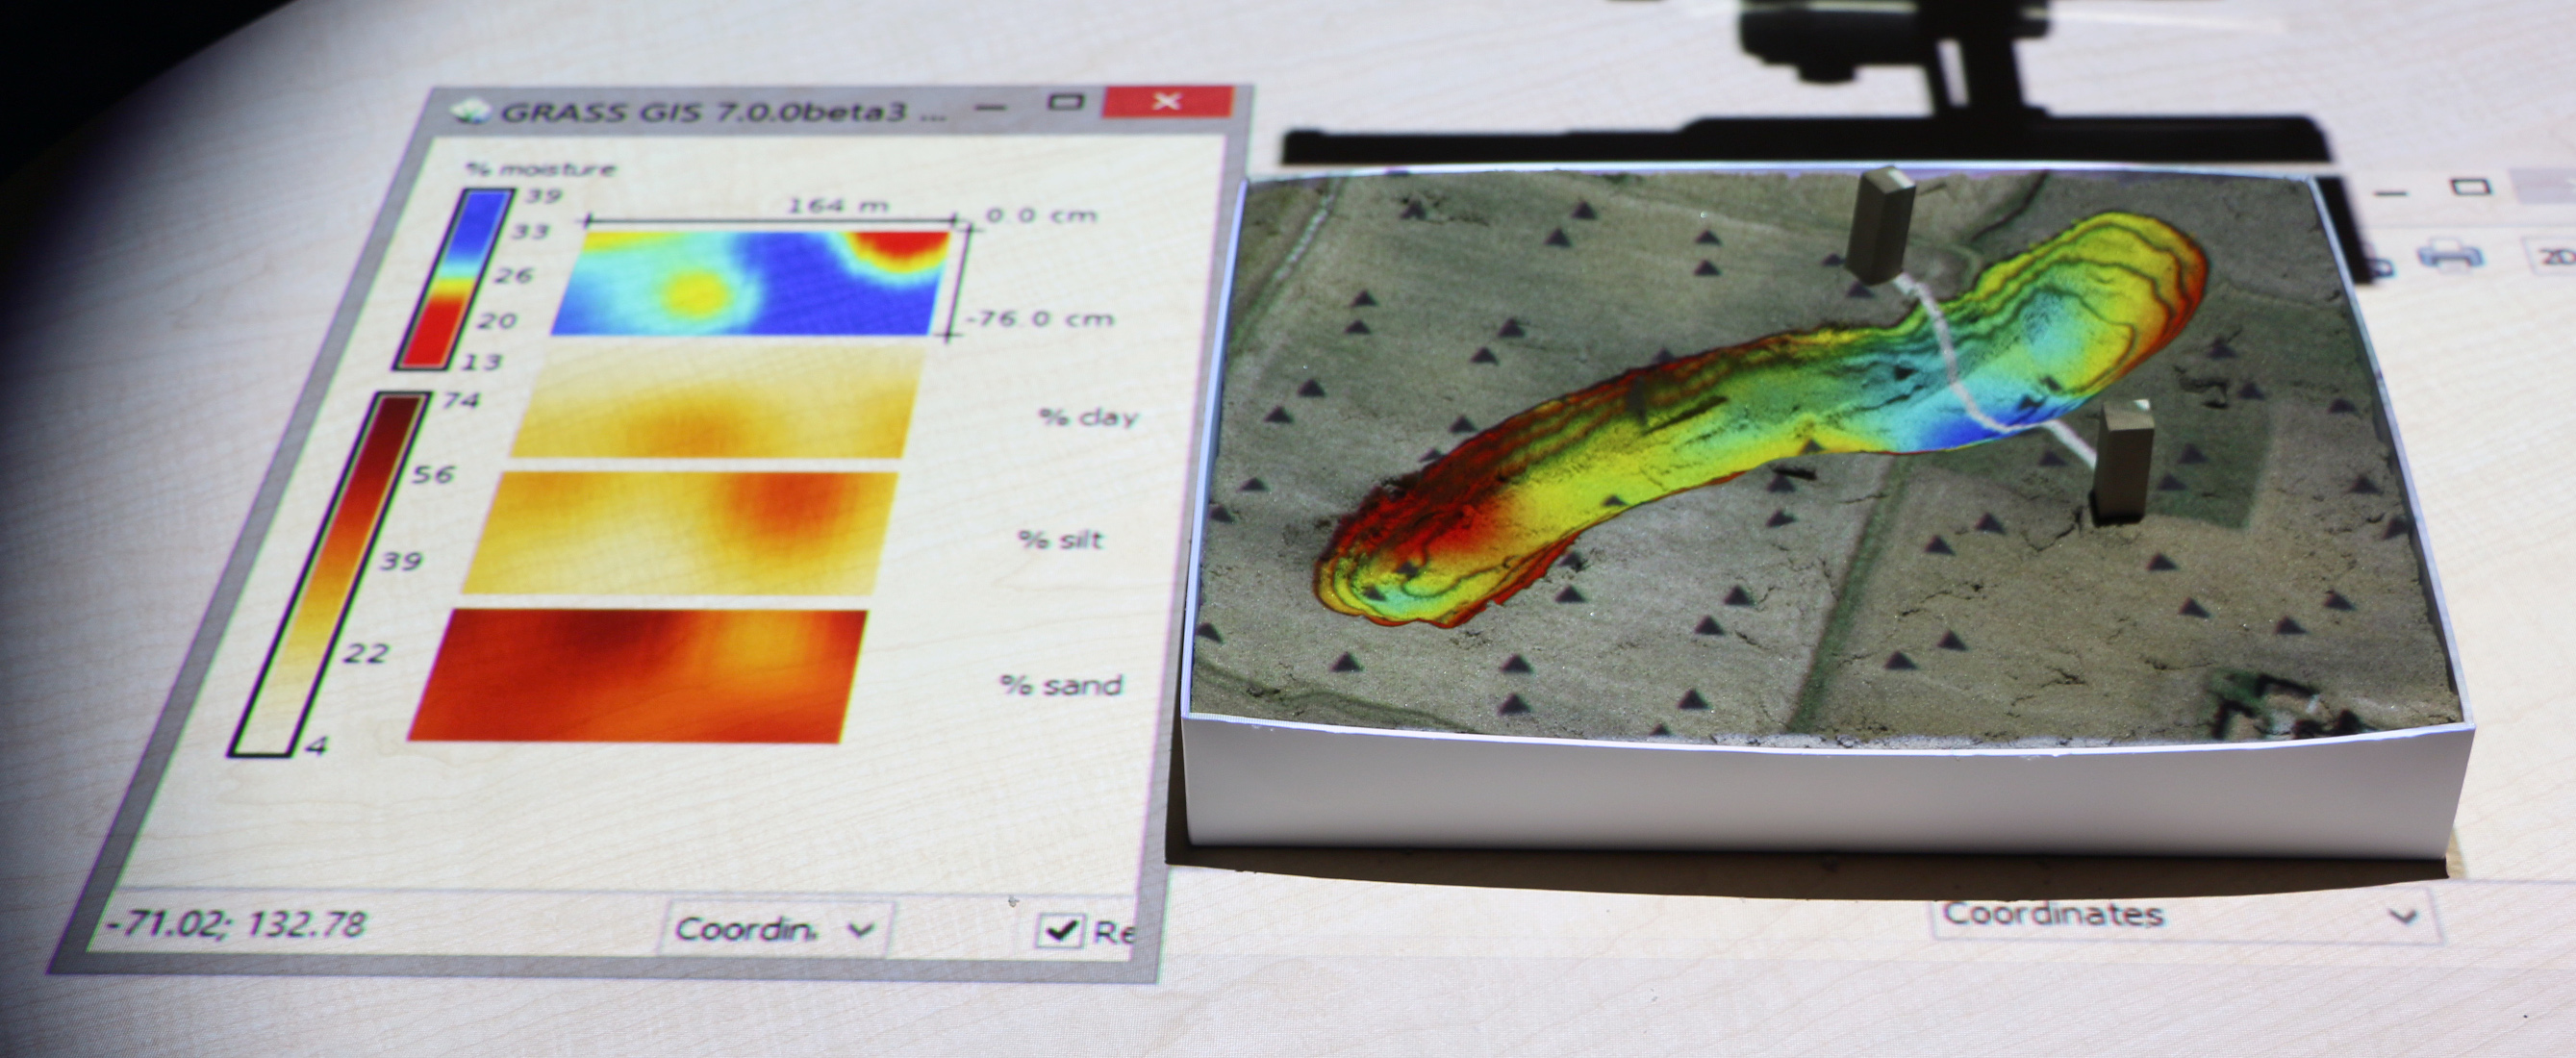
\includegraphics[height=70px]{images/applications/subsurface_3.jpg}
	\caption{Naturally exploring subsurface soil moisture and soil types with Tangible Landscape.}
	\label{fig:subsurface}
\end{center}
\end{figure}

\begin{table}
\tbl{Collaboratively sculpting topography to create lakes, drawing trees with a laser pointer, and visualizing in VR.}{
\ra{1.3}
\begin{tabular}{m{0.49\textwidth} m{0.49\textwidth}}
\toprule
\multicolumn{1}{c}{Sculpting}  & \multicolumn{1}{c}{Drawing \& Immersion}\\
\midrule
%
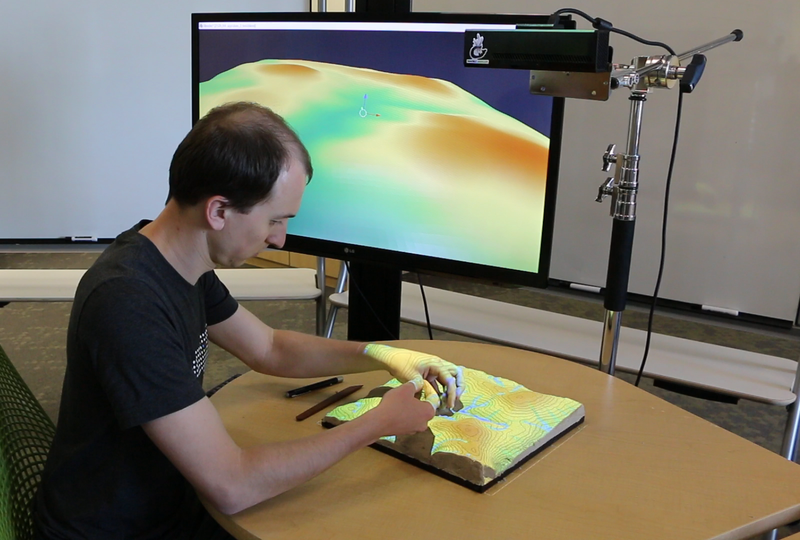
\includegraphics[width=0.49\textwidth]{images/immersive/sculpting_lakes_2.png} &
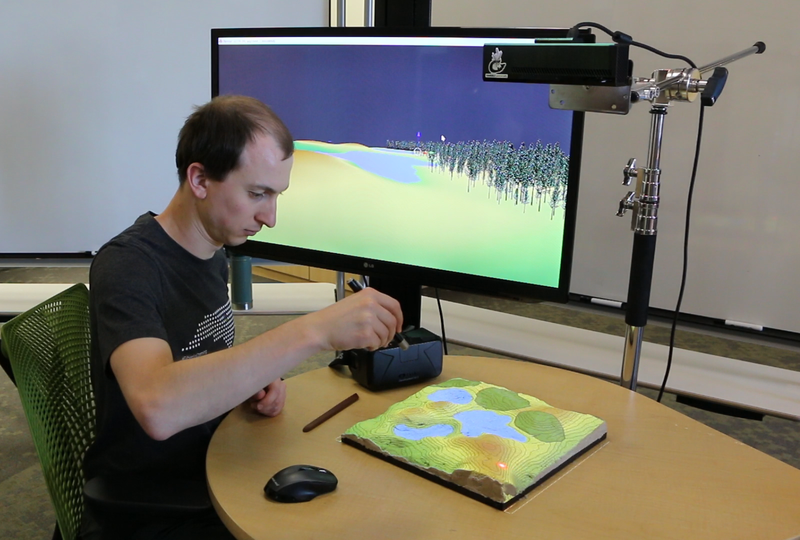
\includegraphics[width=0.49\textwidth]{images/immersive/drawing_trees_1.png}\\
%
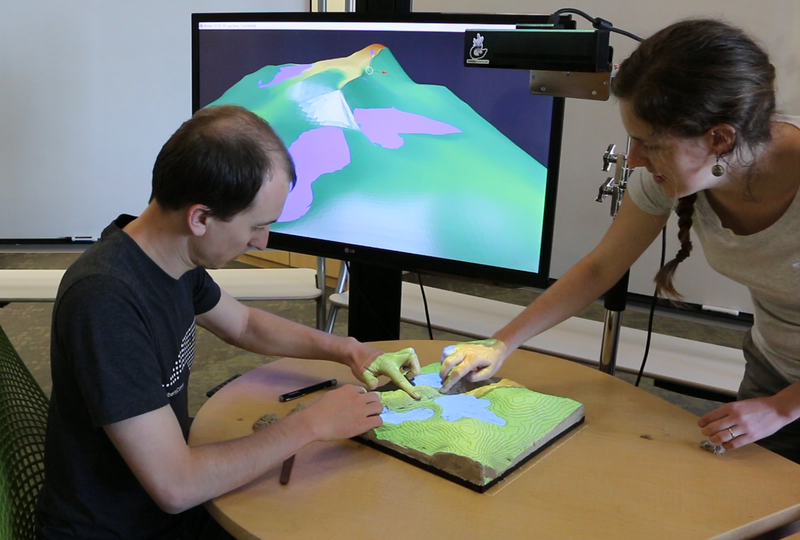
\includegraphics[width=0.49\textwidth]{images/immersive/sculpting_landforms_2.png} &
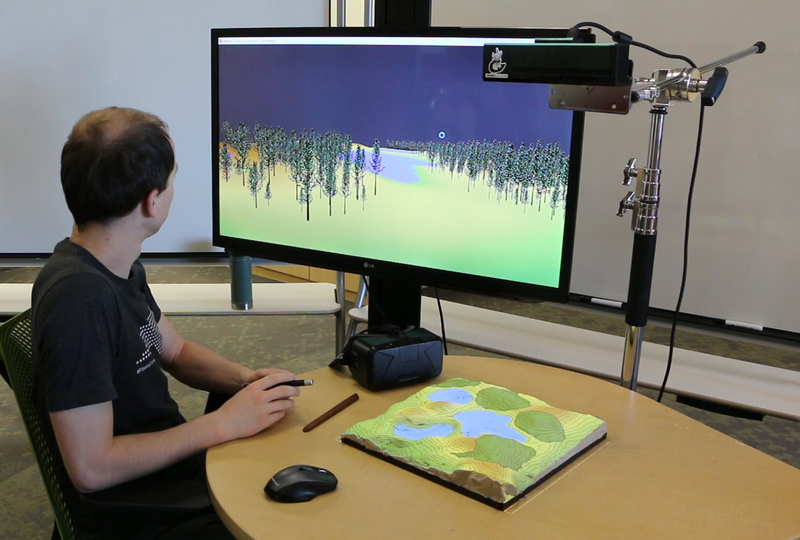
\includegraphics[width=0.49\textwidth]{images/immersive/drawing_trees_2.png}\\
%
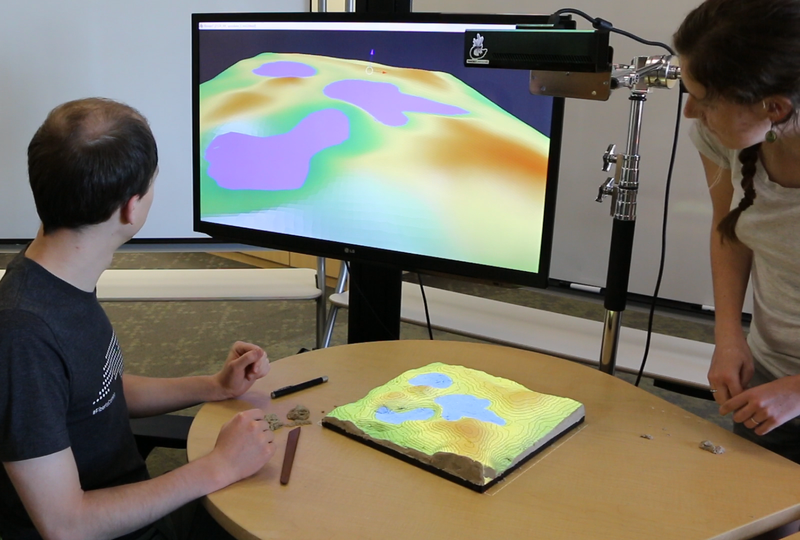
\includegraphics[width=0.49\textwidth]{images/immersive/sculpting_landforms_3.png} &
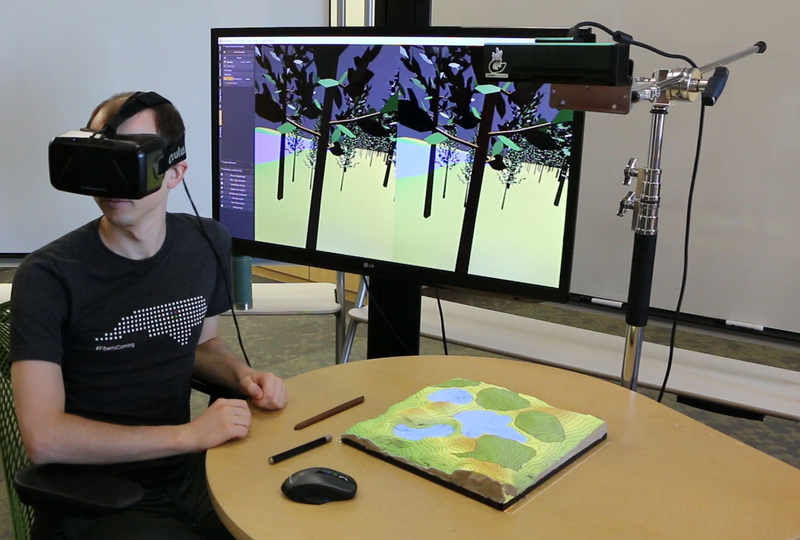
\includegraphics[width=0.49\textwidth]{images/immersive/trees_with_oculus_1.png}\\
%
\bottomrule
\end{tabular}}
\label{table:tl_vr} 
\end{table}

%\begin{figure}
%\begin{center}
%		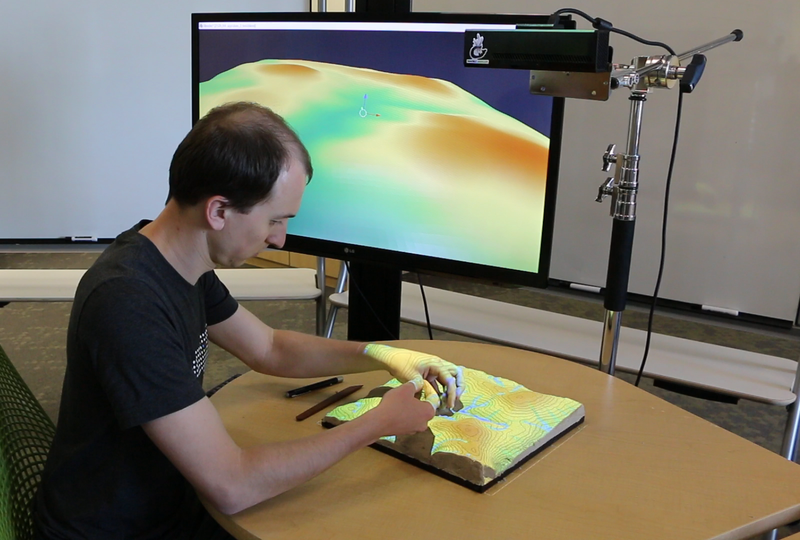
\includegraphics[width=0.32\textwidth]{images/immersive/sculpting_lakes_2.png}
%		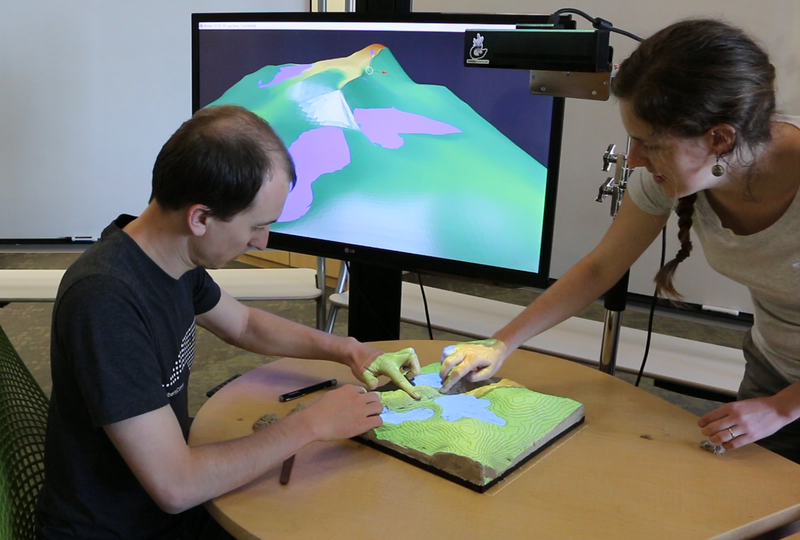
\includegraphics[width=0.32\textwidth]{images/immersive/sculpting_landforms_2.png}
%		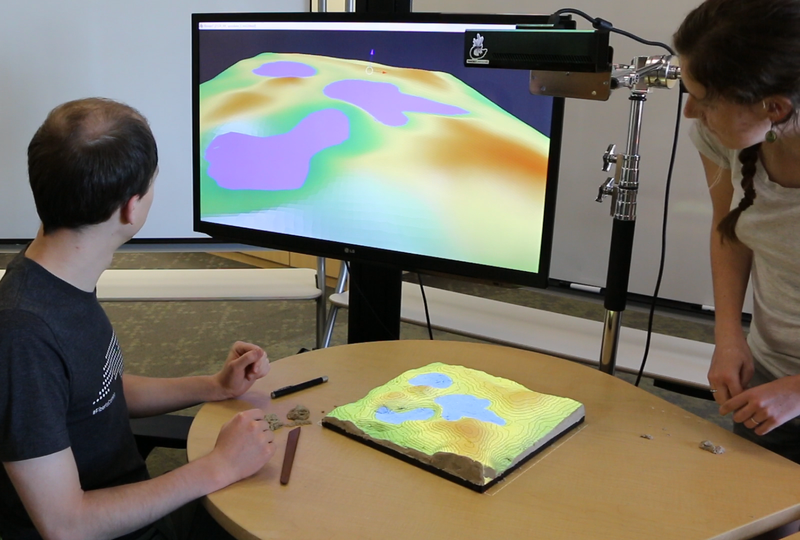
\includegraphics[width=0.32\textwidth]{images/immersive/sculpting_landforms_3.png}
%	\caption{Collaboratively sculpting topography and creating lakes with Tangible Landscape.}
%	\label{fig:collaboration}
%\end{center}
%\end{figure}
%
%\begin{figure}
%\begin{center}
%		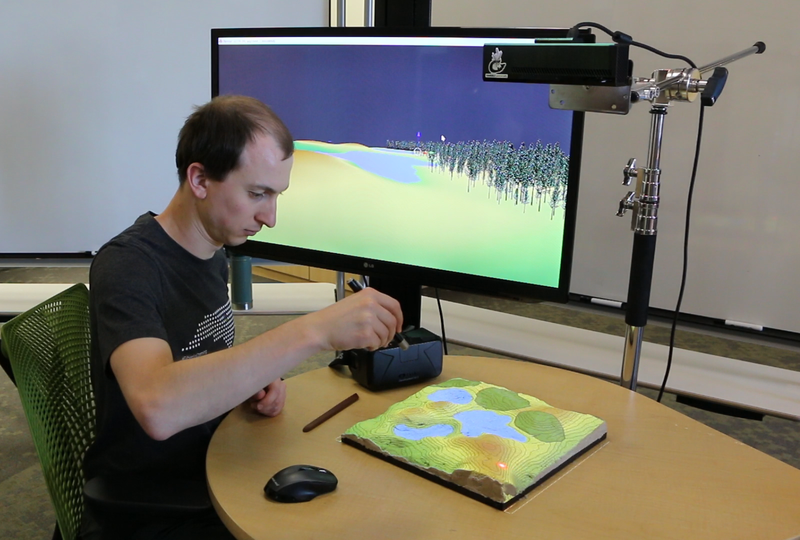
\includegraphics[width=0.32\textwidth]{images/immersive/drawing_trees_1.png}
%		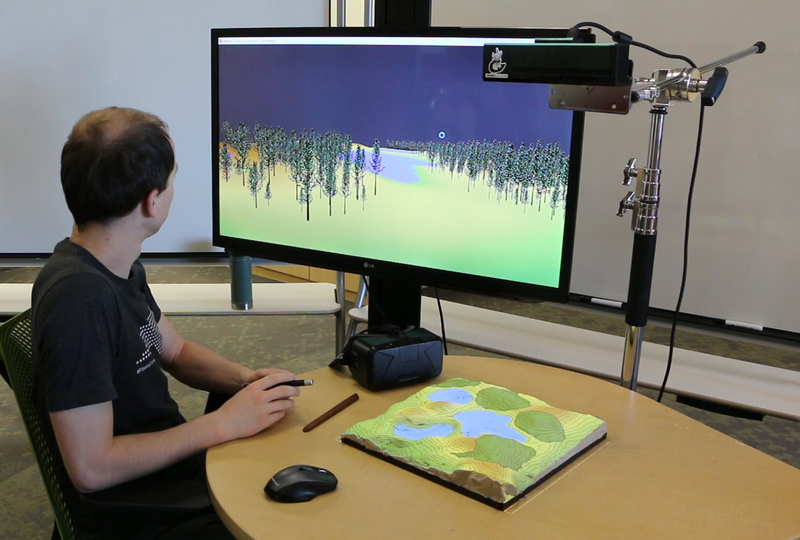
\includegraphics[width=0.32\textwidth]{images/immersive/drawing_trees_2.png}
%		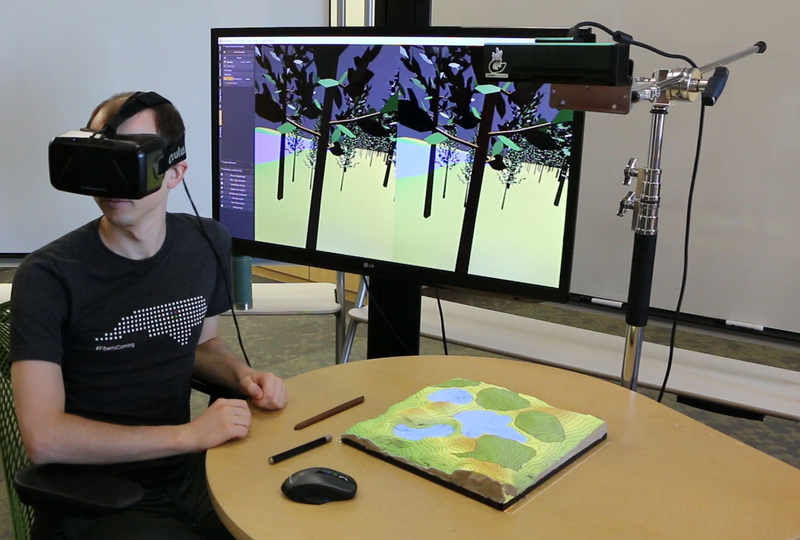
\includegraphics[width=0.32\textwidth]{images/immersive/trees_with_oculus_1.png}
%		%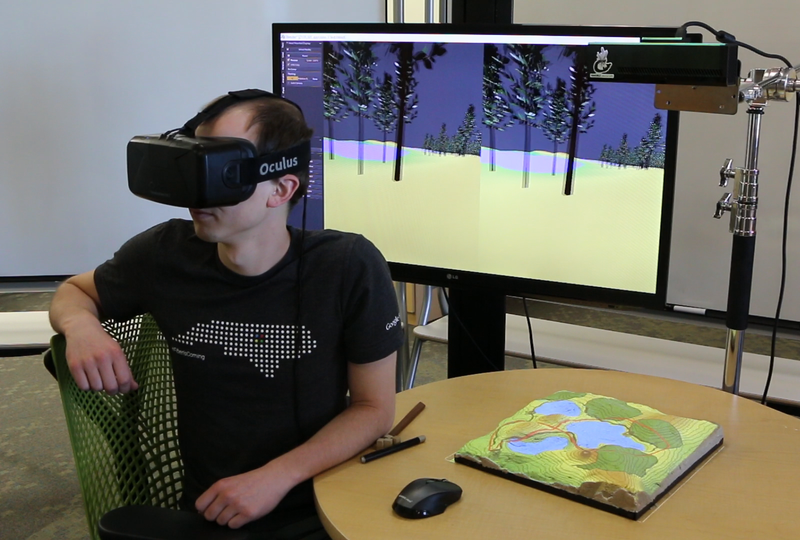
\includegraphics[width=0.32\textwidth]{images/immersive/walkthrough_2.png}
%	\caption{Drawing and visualizing trees using a laser pointer with Tangible Landscape and an Oculus Rift.}
%	\label{fig:drawing_trees}
%\end{center}
%\end{figure}

\paragraph{Multidimensional sketching}
%
Tangible Landscape was designed to enable tangible multidimensional sketching
in geographic space and time. 
%
With Tangible Landscape users can sketch in 3D
by sculpting surfaces or volumes,
drawing across surfaces, 
or placing and manipulating 3D objects.
%
By directly manipulating 3D form 
users can indirectly shape other dependent dimensions of data 
such as simulated processes. 
%
Each scan can be stored, timestamped, and registered
as a space time raster or vector dataset % spatiotemporal dataset
in GRASS GIS' temporal framework
to create a time series of maps. 
%
With this time series users can animate the evolution of their model using the module 
\emph{g.gui.animation}\cite{g.gui.animation}.

% add animated video with example

Advances in virtual reality are enabling immersive 3D sketching.
%
The illustrator
Wesley Allsbrook, %and the Oculus Story Studio team have
for example, 
has drawn an animated short film called Dear Angelica
by sketching in 3D space using the Oculus Rift and Oculus Touch
to combine the affordances of digital painting and physical sculpture \cite{Oculus2016,Quilez2016}. 
%
While this sort of immersive 3D sketching is situated in a fully virtual space,
tangible 3D sketching is situated in a real, but digitally augmented space. 
%
Tangible 3D sketching
can be situated in a collaborative social context
and may not require any new skills -- 
for tangible interactions 
%such as 3D sketching 
can be analogous to everyday actions, 
making use of existing motor schema.
%
While these approaches to 3D sketching 
should theoretically offer very different affordances
in terms of embodied and situated cognition
both have the potential to revolutionize how we 
express ourselves in space and time.

\subsection{Implementation}

% ---------------------------- REVISIONS ---------------------------- 
% 
% Describe system implementation in greater detail
% 	Physical dimensions
% 		Diagram of system with dimensions
% 	Capturing distance
% 		Precision
% 		Scanning res in x, y, z
% 		Noise
% 	Sampling rate
% 	Filtering
% 	Lag
% 		Lag due to analyses
% 			Table of analyses with speed benchmarks
% 		Discussion of frame rate and interaction
% 			Tradeoffs 
% 
% -------------------------------------------------------------------------- 

% EDITOR: Add details on the system implementation. While we understand that the system is not the main contribution here, it is important to describe it in sufficient details. Please add physical dimensions, capturing distances, lag, what contributes to 2 sec. delay?, etc.

% REFEREE 1: From a technical point of view, the presented system seems to be a solid piece of work. Yet, the authors do not describe it in detail. Thus technical aspects cannot be judged (compared to the state of the art) very well. One side remark on page 24 states that the feedback rate how has (only) two seconds of lag. Is this fast enough for users to work interactively?

% REFEREE 2: 
%Some key parameters of the system setup should be included:
%- What is the physical size of the sand interface?
%- At the mounted distance of the Kinect, what is the scanning resolution in x,y, and z, and how much noise does the sensor produce? What is the sampling rate? Does the system filter and average the sensor data over time or drop frames and only use raw data?
%- What is the system lag? The article mentions an improved subsequent system with a 2 second delay in the end, but does not state the delay for this system in the study. System lag seems like a critical factor for the projected feedback in the difference experiment and the water flow experiment. What are the observations of the authors in this regard? I suspect that a low framerate may be even helpful in some conditions, as it produces fewer distractions than a fast, noisy visual feedback.

Tangible Landscape uses Microsoft Kinect to continuously capture the shape of the physical model
as a point cloud and processes it into a raster-based DEM in GRASS GIS database.
Since the scanner can be slightly tilted,
we first ensure the scan is horizontally aligned by a calibration process, which derives
a rotation matrix by scanning a horizontal surface of the table where the model lies.
This rotation matrix is then applied for each scan.
The point cloud is automatically trimmed to include only points on the physical model,
smoothed and georeferenced based on the known
spatial extent of the area represented by the model.
Georeferencing includes translation, rotation by 180\textdegree{} along z axis,
and separate horizontal and vertical scaling, where vertical scaling takes into
account possible vertical exaggeration of the physical model.
The resulting terrain representation has real world dimensions
and can be combined effortlessly with other GIS data, such as land cover or orthophotograph.

The DEM is then reconstructed from the point cloud either using interpolation method
with regularized spline with tension \cite{Mitasova2005},
or binning with cell values computed as the mean of points' z coordinates falling into that cell.
Although binning results in noisier DEM, it is very fast,
and can therefore be a better option for certain applications. 
Multiple point clouds can be integrated to increase point density at the cost of increased
processing time.

For each new DEM, a set of customizable analyses and geospatial workflows
specified in a Python file is run, and the display is updated.
Tangible Landscape provides a library of geospatial functions built on top of
GRASS GIS modules and an API for developing custom workflows.
The modeled analyses as well as scanning parameters can be modified 
as the system runs.



Tangible Landscape has been implemented as a set of components 
-- the \emph{r.in.kinect} add-on module \cite{r.in.kinect}
%\footnote{\url{https://github.com/tangible-landscape/r.in.kinect}}
and the \emph{Tangible Landscape} plugin \cite{grass-tangible-landscape}
%\footnote{\url{https://github.com/tangible-landscape/grass-tangible-landscape}}
--
for the active development version of GRASS GIS (Fig.~\ref{fig:software_schema}). 
The \emph{r.in.kinect} add-on module continuously imports and filters point cloud data from the \nth{2} generation Kinect into GRASS GIS as raster or vector maps. 
It has been implemented as a separate component so that it can easily be used for other applications.
The \emph{Tangible Landscape} plugin provides 
utilities, a library of analyses, and a GUI dialog for tangible interaction in GRASS GIS.
The \emph{Tangible Landscape Immersive Extension} \cite{tangible-landscape-immersive-extension}
%\footnote{\url{https://github.com/tangible-landscape/tangible-landscape-immersive-extension}}
links Tangible Landscape with Blender, 
an open source 3D modeling and animation program \cite{Blender} 
enabling 3D rendering on screens or head-mounted displays.

Users can develop new analyses for Tangible Landscape 
using the GRASS GIS Python Scripting Library.  %GRASS GIS Python API
Since many tasks in GIS are not appropriate for tangible interaction
Tangible Landscape was designed to supplement, 
not replace GRASS GIS's GUI, CLI, and scripting application program interface (API). 
Tangible Landscape currently runs on Linux and Mac OSX.
%with an unsupported branch for Windows. 
Dependencies include the Point Cloud Library \cite{Rusu2011,PCL}, 
OpenKinect's libfreenect2 \cite{OpenKinect}, 
OpenCV \cite{OpenCV},  
watchdog \cite{watchdog}, 
and GRASS GIS \cite{GRASS_GIS_software}.

\begin{figure}
\begin{center}
		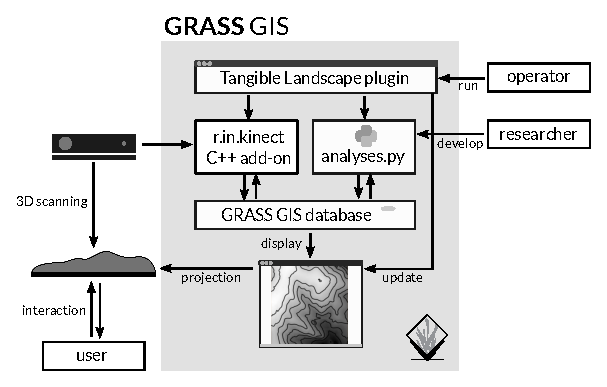
\includegraphics{images/software-schema.pdf}
	\caption{Software schema for Tangible Landscape.}
	\label{fig:software_schema}
\end{center}
\end{figure}

\subsection{System resolution, accuracy, and speed}
The spatial resolution of the system is determined by the depth camera parameters
and the distance from camera to the model. Given Kinect's field of view of 70 $\times$ 60 degrees
and depth resolution of 512 $\times$ 424 pixels, the spatial resolution ranges
from 1.4 to 2.7 mm for distances from 0.5 to 1 m used typically by Tangible Landscape.
For the experiment where the distance was approximately 0.6 m we used 2 mm resolution, which
translated to 6 m in real world given the scale of the physical model.
Kinect depth measurements suffer from noise quantified by \cite{Hamed2015}.
We minimized the negative effects of noise by placing the model
closer to the center of the camera and by smoothing the data using Moving Least
Squares reconstruction method \cite{Rusu2011}.

In Fig.~\ref{fig:accuracy} and Table \ref{table:accuracy} 
we show the accuracy of the experiment setup.
We scanned a CNC routed model used in this study
and compared it with the original DEM.
% do we know the accuracy of cnc? 
% 0.125" or 3.175 mm bit with 0.05" or 1.27 mm stepover with +- 0.01 mm positional accuracy
% so could say 1.27 mm +- 0.01
The routed model is sufficiently accurate for this comparison.
We removed the systematic error (vertical shift) since it is removed
during processing of the scans from the experiment and does not influence the results.
The difference in Fig.~\ref{fig:accuracy} is given from a single frame,
and although it is possible to integrate multiple frames,
we chose to construct the DEM from one frame for faster smoothing procedure.

% This table might not be needed given the histogram on the legend

\begin{figure}
\begin{center}
		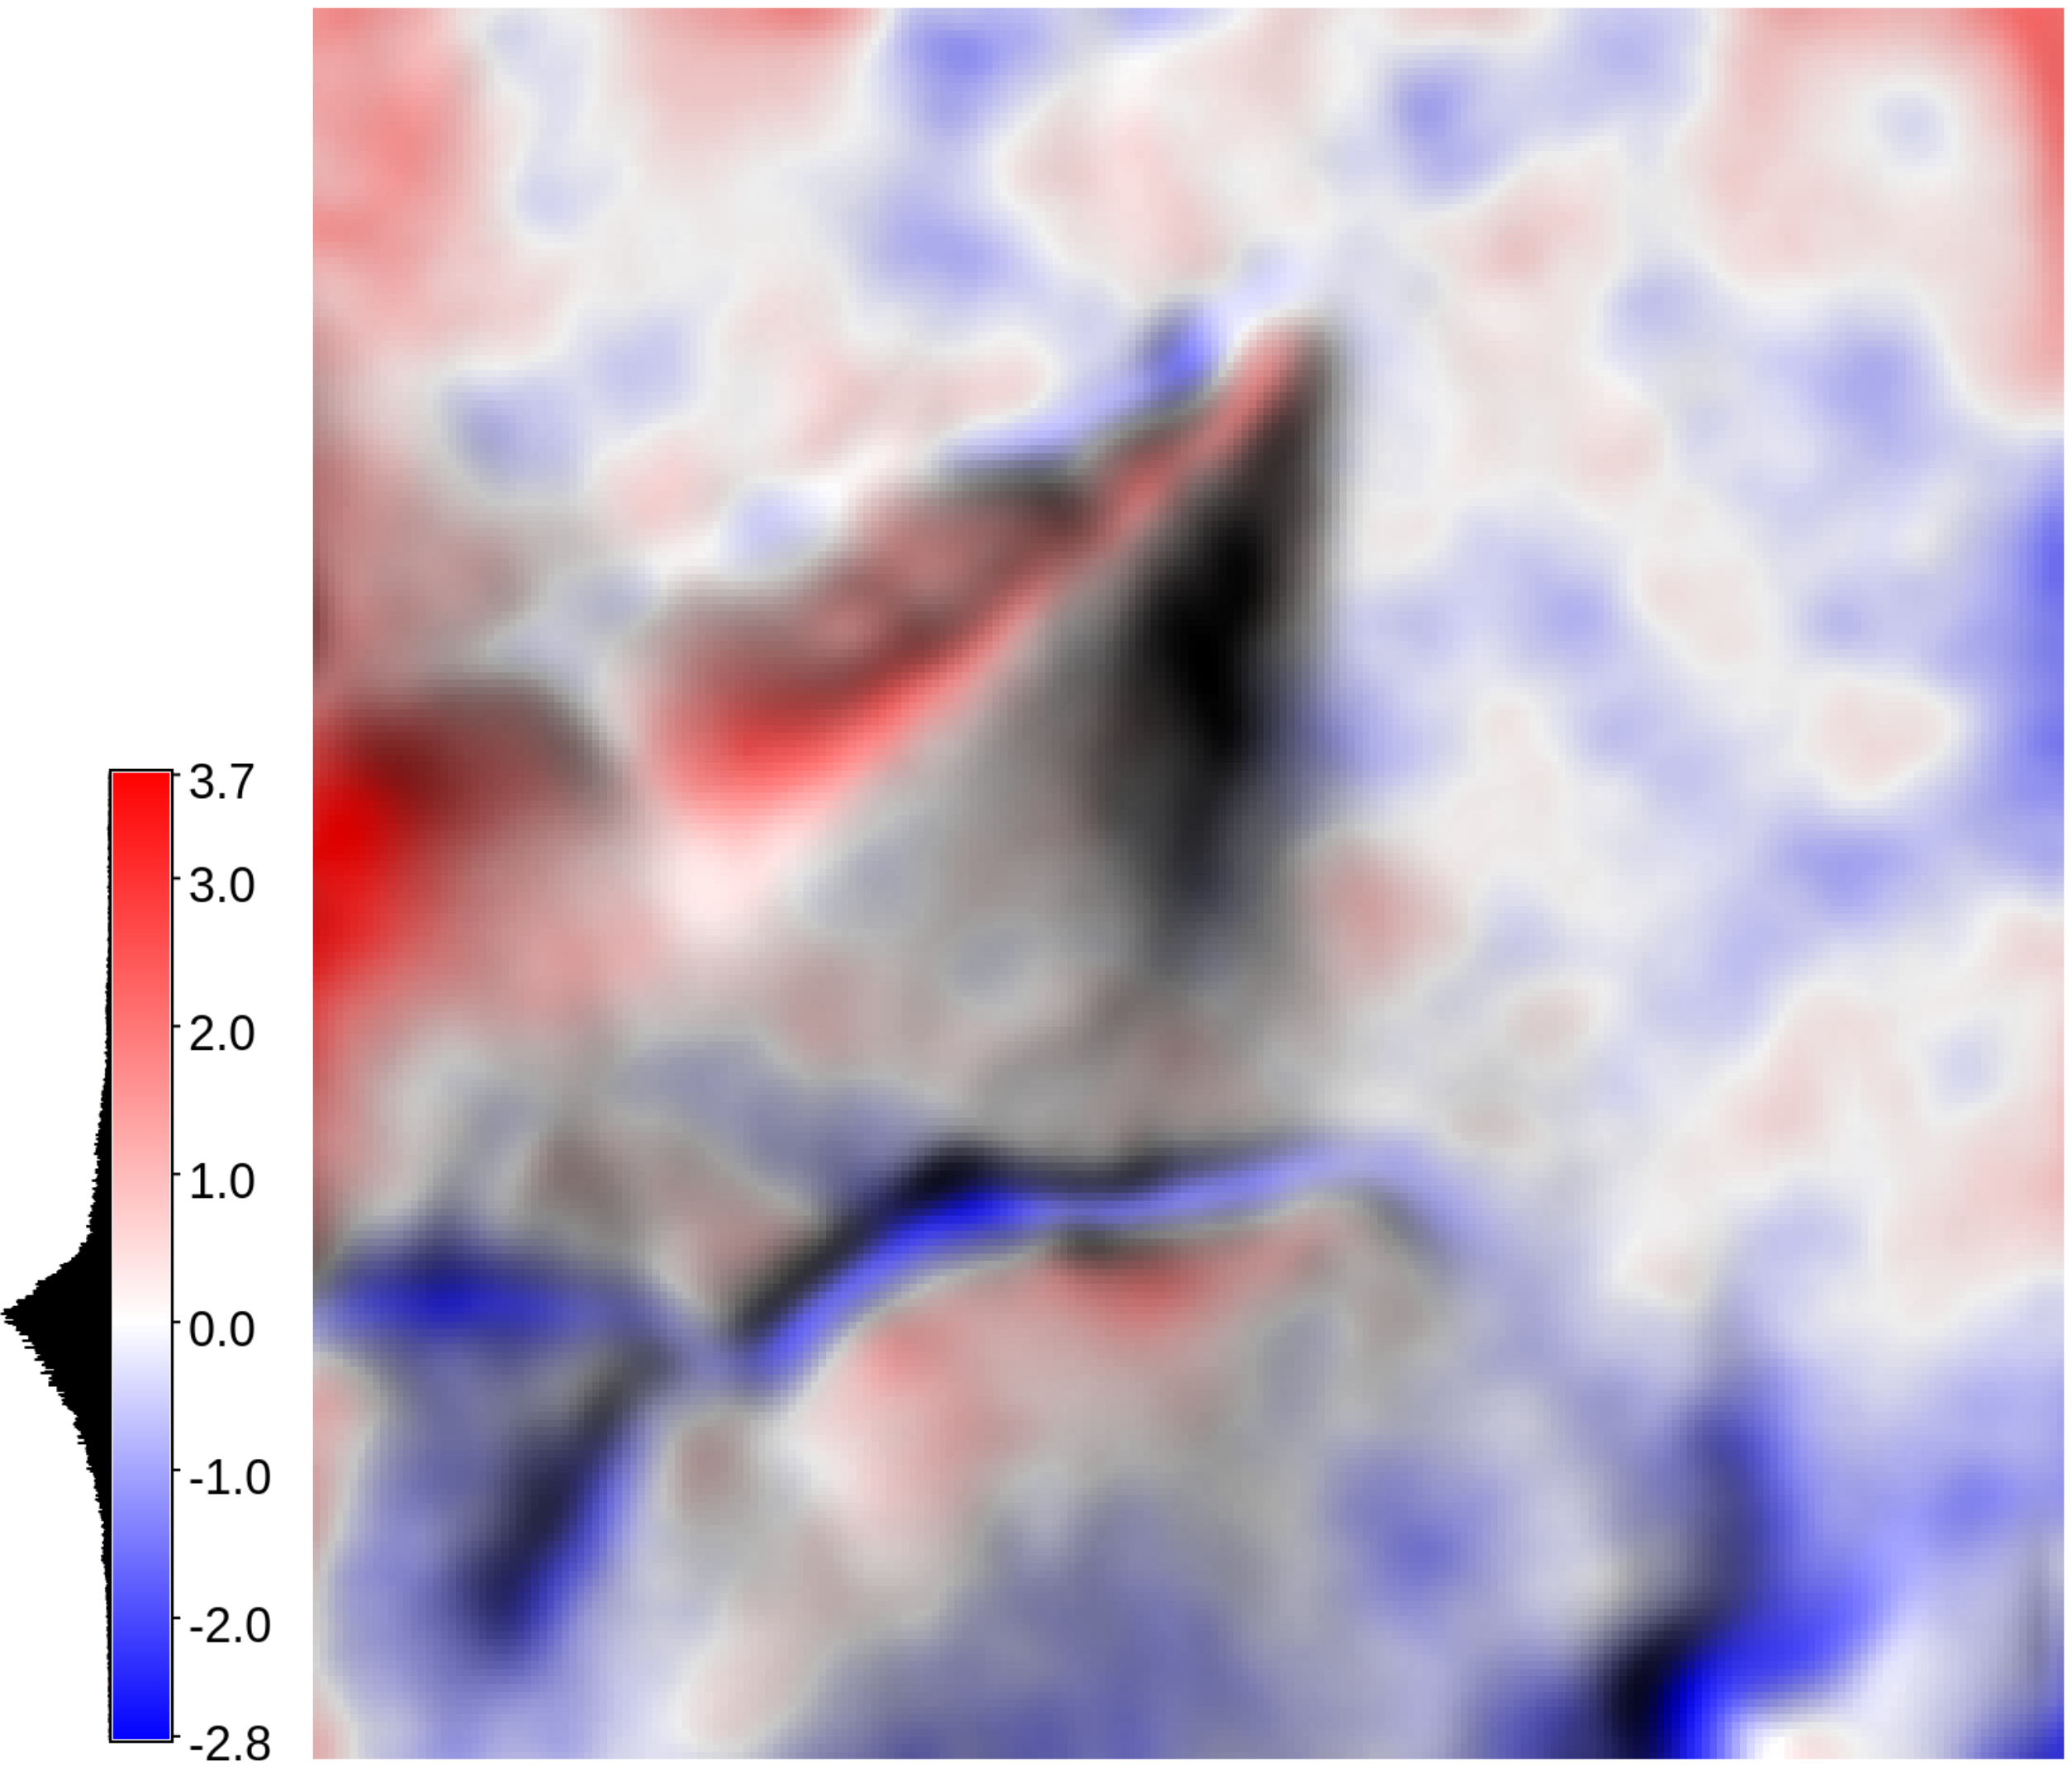
\includegraphics[width=0.6\textwidth]{images/precision/accuracy.png}
	\caption{Accuracy assessment: difference between original DEM and the scanned DEM of a model representing the DEM.
	The scanned DEM is higher then the original DEM in blue areas and lower in red areas. Legend values are in millimeters.
	}
	\label{fig:accuracy}
\end{center}
\end{figure}

\begin{table}
\tbl{Scanning accuracy}{
\ra{1.3}
\begin{tabular}{c <{\hspace{1em}} c <{\hspace{1em}} c <{\hspace{1em}} c <{\hspace{1em}} c <{\hspace{1em}} c}
\toprule
Min & Max & Mean & Stdev &  \nth{1} Q & \nth{3} Q\\
\midrule
-2.8 & 3.7 & -0.02 & 0.7 & -0.4 & 0.3\\
\bottomrule
\end{tabular}}
\label{table:accuracy} 
\end{table}

% r.in.kinect smooth=10
\begin{table}
\tbl{Scanning speed}{
\ra{1.3}
\begin{tabular}{l <{\hspace{1em}} c <{\hspace{1em}} c <{\hspace{1em}} c <{\hspace{1em}} c <{\hspace{1em}} c}
\toprule
Size, Process & Small & Medium\\
\midrule
% Resolution & 6 $\times$ 6 m & 4.32 $\times$ 4.24 \\
Physical size & 23.5 cm $\times$ 23.5 cm & 34 cm $\times$ 34 cm \\
% Cells & 116 $\times$ 116 & 159 $\times$ 165 \\
Cells & 13,456 & 26,235 \\
Binning & 0.51 s & 0.71 s \\
Interpolation & 0.74 s & 0.97 s \\
% r.sim.water stop in 5 iterations on iterpolated
Water flow & 0.29 $\pm$ 0.01 s & 1.05 $\pm$ 0.05 s \\
% r.contour 106-150 2m interval
Contours & 0.054 $\pm$ 0.004 s & 0.061 $\pm$ 0.004 s \\
% r.mapcalc 'a-b' and r.colors (plain, no histogram eq)
Difference & 0.036 $\pm$ 0.002 s & 0.042 $\pm$ 0.003 s \\
% r.geomorphon search=22 skip=12
Landforms & 0.034 $\pm$ 0.003 s & 0.084 $\pm$ 0.009 s \\
\bottomrule
\end{tabular}}
\label{table:benchmark}
\end{table}

Tab.~\ref{table:benchmark} shows comparison of times for different point cloud processing
methods (binning and interpolation) and analyses (e.g. water flow analysis).
The small model is the size used in the study.
The medium model corresponds to what we recommend as a basic size for Tangible Landscape beginners.
The time needed to scan and obtain a model is under 1~s,
however the subsequent one or more analyses may take more than 1~s.
Considering computation of the water flow and the smaller model,
the minimal total time needed for change to be reflected
is the time of the interpolation 0.74~s plus the time of the water flow analysis 0.29 s
which gives is 1.03~s.
The maximum total time which considers that the person interacting with Tangible Landscape
made a change right after the scan was performed is 2.06 s because it includes waiting
for the previous scan to be processed.
It must be noted that the system used for the study had worse performance than
the current, reported system.
% TODO: include the approx time for the old system
Benchmarks were performed using
System76 Oryx Pro with
% 3.5 GHz Quad-Core
6th Generation Intel Core processor i7-6700HQ (2.6 GHz, up to 3.5 GHz, 6 MB cache 4 cores, 8 threads),
16 GB dual-channel DDR4 random-access memory (2 $\times$ 8 GB),
% (RAM is in GB, not GiB)
M.2 SSD storage (540 MB/s sequential read, 520 MB/s write), and
NVIDIA GeForce GTX 1060
running Ubuntu 16.04 LTS (64-bit),
GRASS GIS 7.2, and
Tangible Landscape 2c1ede9.


\subsection{Fabrication}
We typically use familiar, everyday materials 
-- like sand and wooden blocks -- 
for modeling with Tangible Landscape. 
Interactions -- like sculpting sand and moving wooden blocks -- 
are analogous to everyday tasks
so users should subconsciously know what to do and how to do it, 
leveraging existing sensorimotor schemas. 
The materiality -- the feel, look, and physics -- of the media matters. 
The choice of material can afford different interactions
and mediate meaning, emotion, and motivation. 
We typically use a polymer-enriched sand for the physical terrain model
so that users can easily sculpt forms in a deformable medium 
that will hold its shape, has good plasticity, and has a familiar feel and aesthetic. 
Digital fabrication technologies 
like computer numeric control (CNC) manufacturing and 3D printing
can be used to create molds for casting polymer-enriched sand 
into precise yet deformable models (Fig.~\ref{fig:casting}). 
Cast sand models can precisely represent complex forms 
that are challenging to model by hand 
and can easily be re-cast after use.

Tangible Landscape can be also be used as a modeling aid for sculpting.
Static projections or dynamic analytics like differencing or water flow 
can be used as guides for hand sculpting terrain models. 
Users can project their target digital elevation model and contours 
over their polymeric sand model as a static guide for sculpting. 
Tangible Landscape can also dynamically compute the difference -- i.e.\ cut and fill --
between the target digital elevation model and the scanned model that has been sculpted . 
The difference can provide a real-time guide 
where to add or remove sand in order to match the target digital elevation model (Fig.~\ref{fig:difference_sequence}). 

\begin{figure}
\begin{center}
		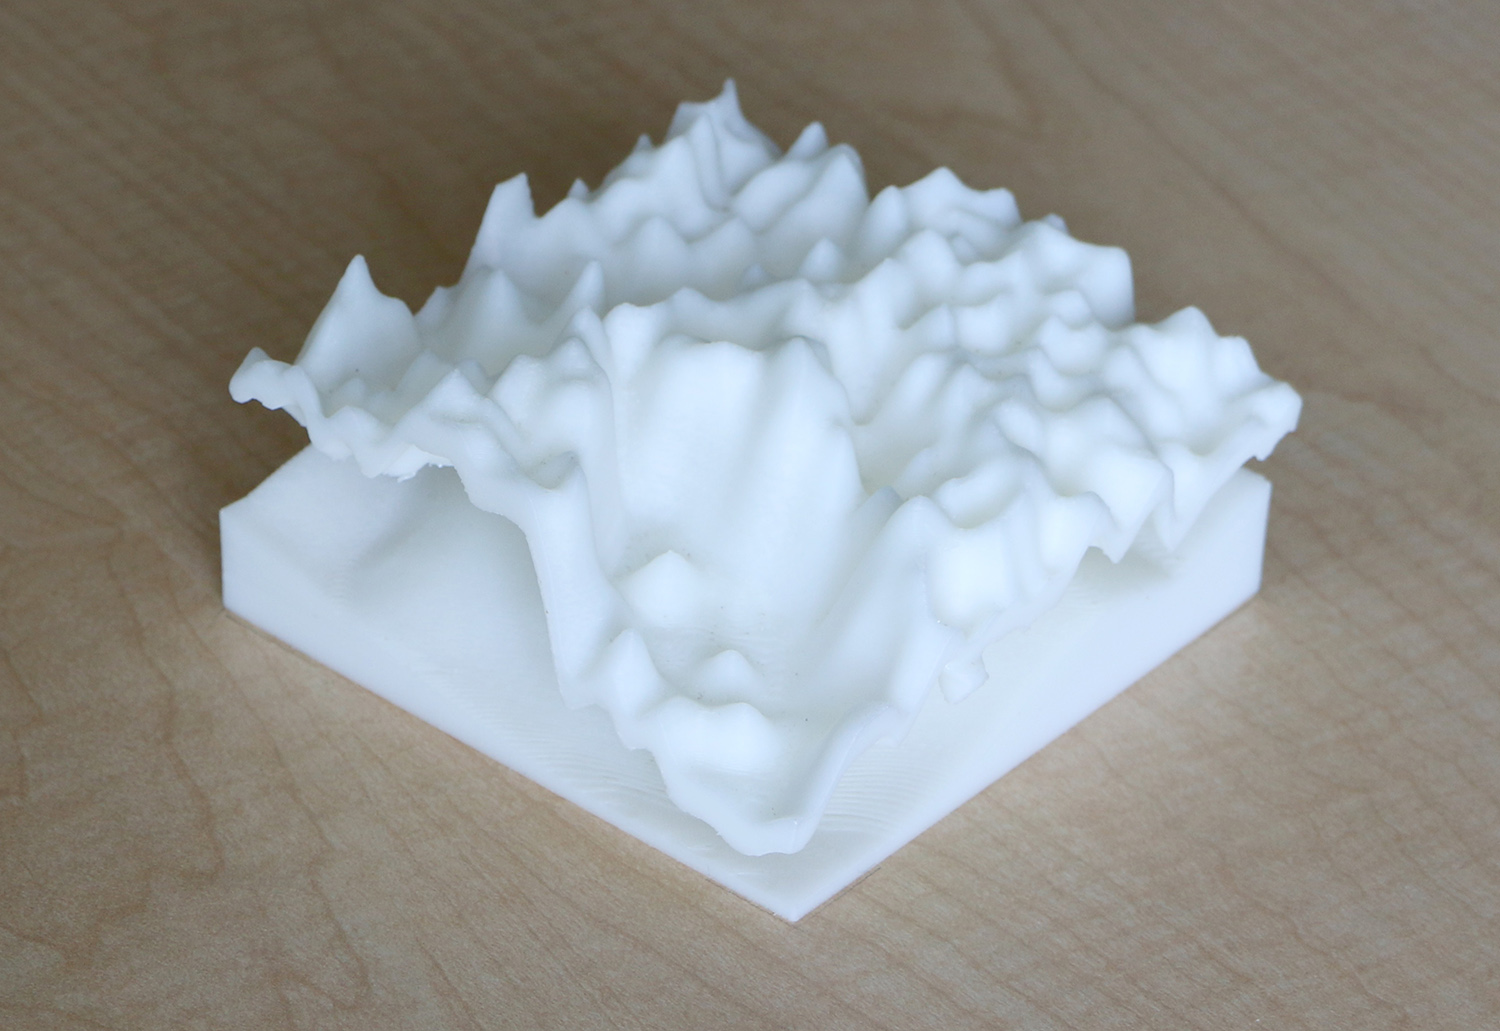
\includegraphics[width=0.32\textwidth]{images/3d_print/3d_print_1.jpg}
		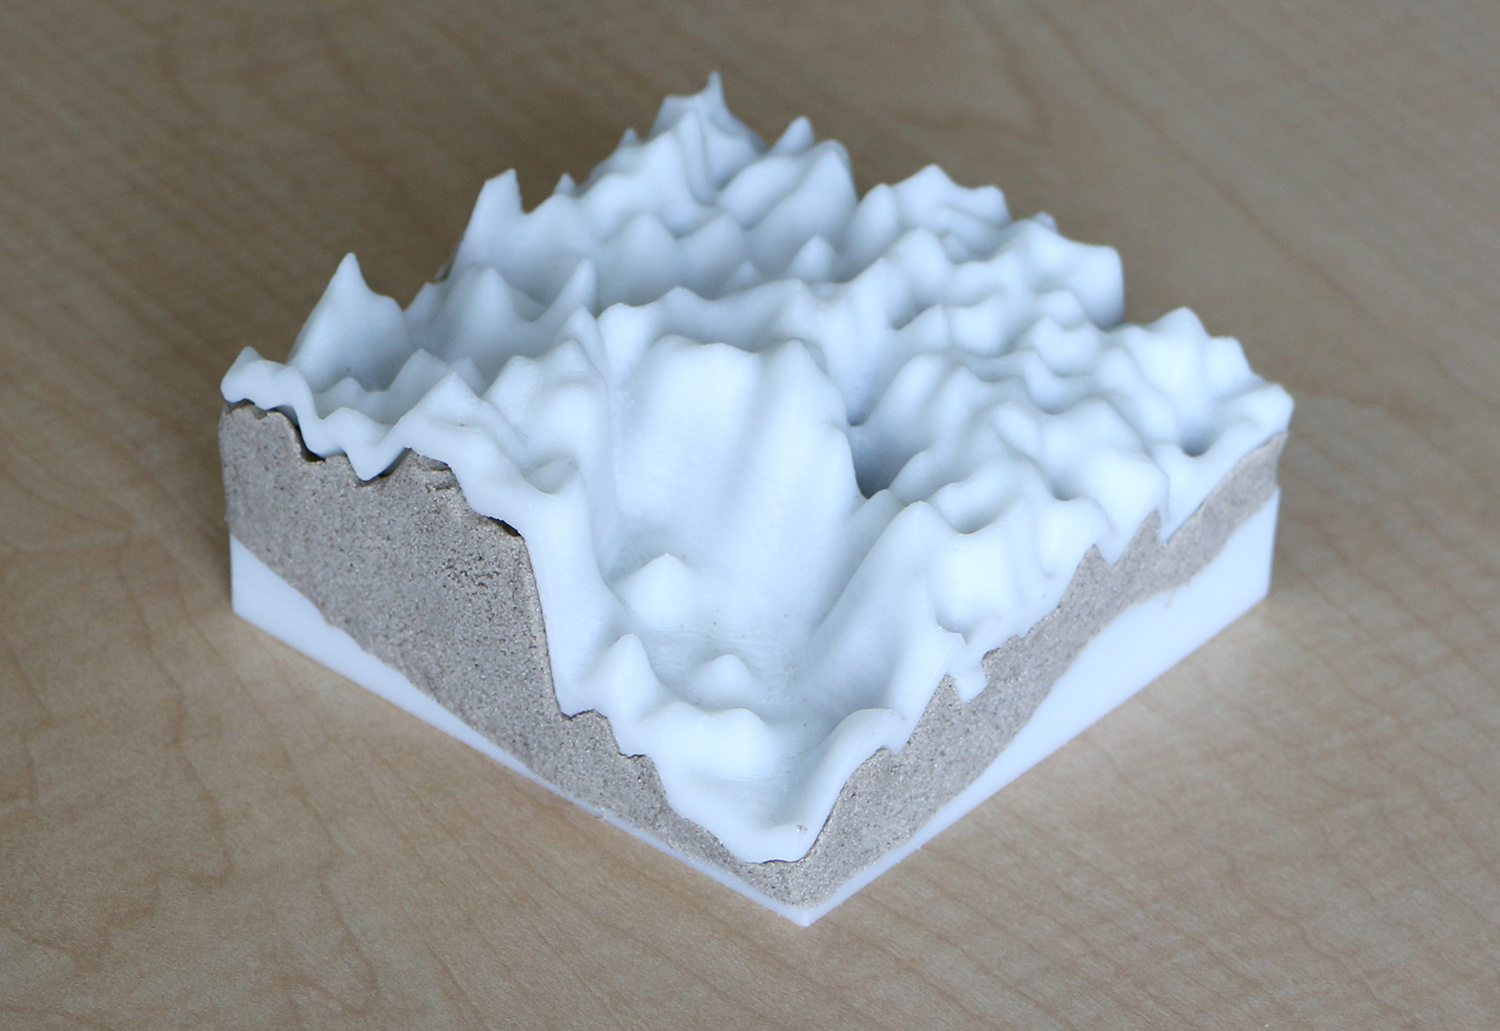
\includegraphics[width=0.32\textwidth]{images/3d_print/3d_print_2.jpg}
		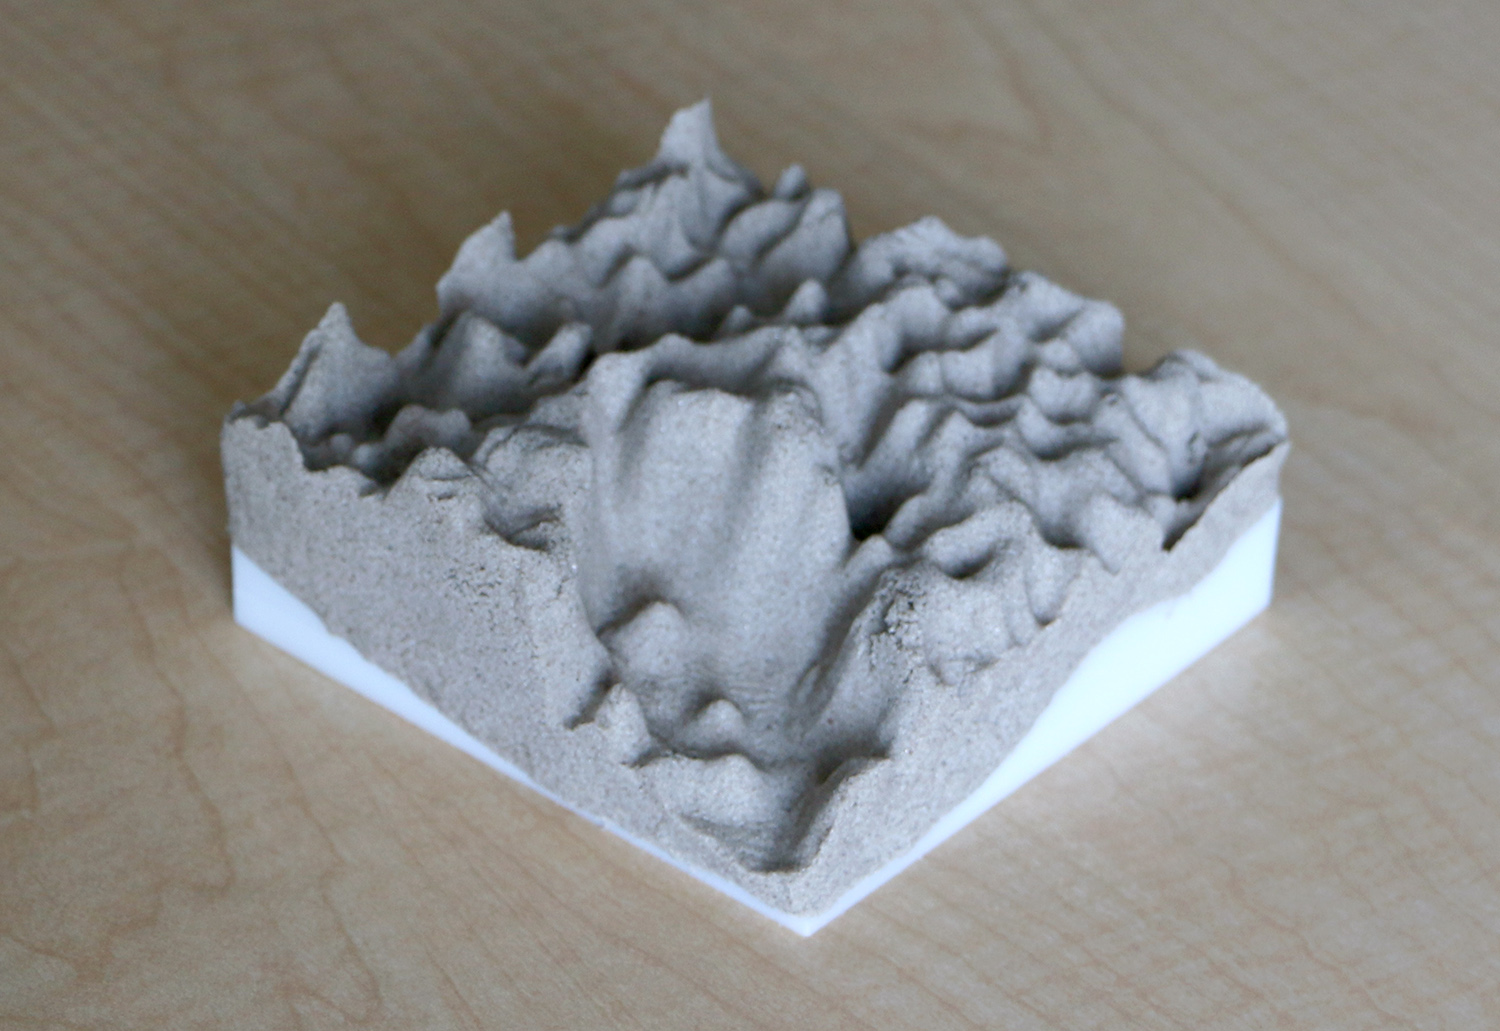
\includegraphics[width=0.32\textwidth]{images/3d_print/3d_print_3.jpg}
	\caption{Casting polymeric sand models with 3D printed molds. Source: \cite{Petrasova2015}.}
	\label{fig:casting}
\end{center}
\end{figure}

\begin{figure}
\begin{center}
		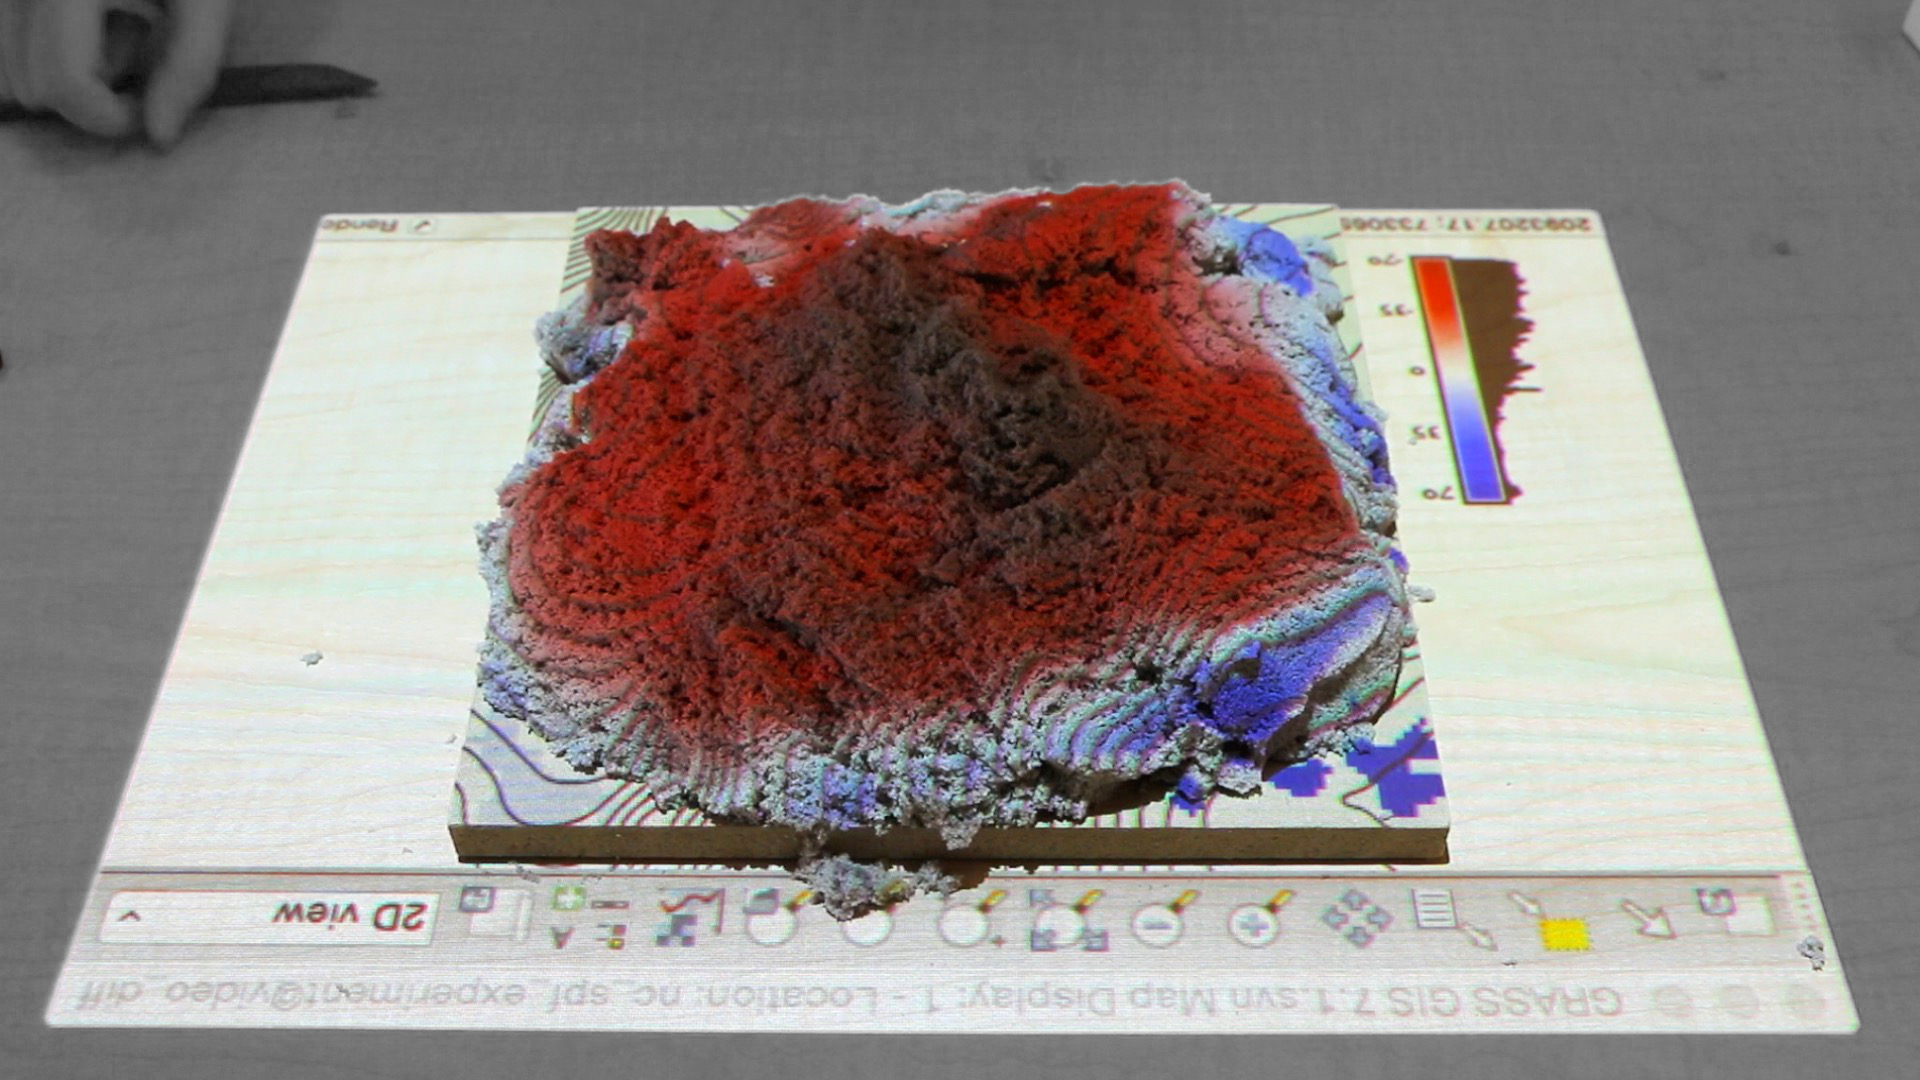
\includegraphics[width=0.49\textwidth]{images/difference/tl_difference_1.jpg}
		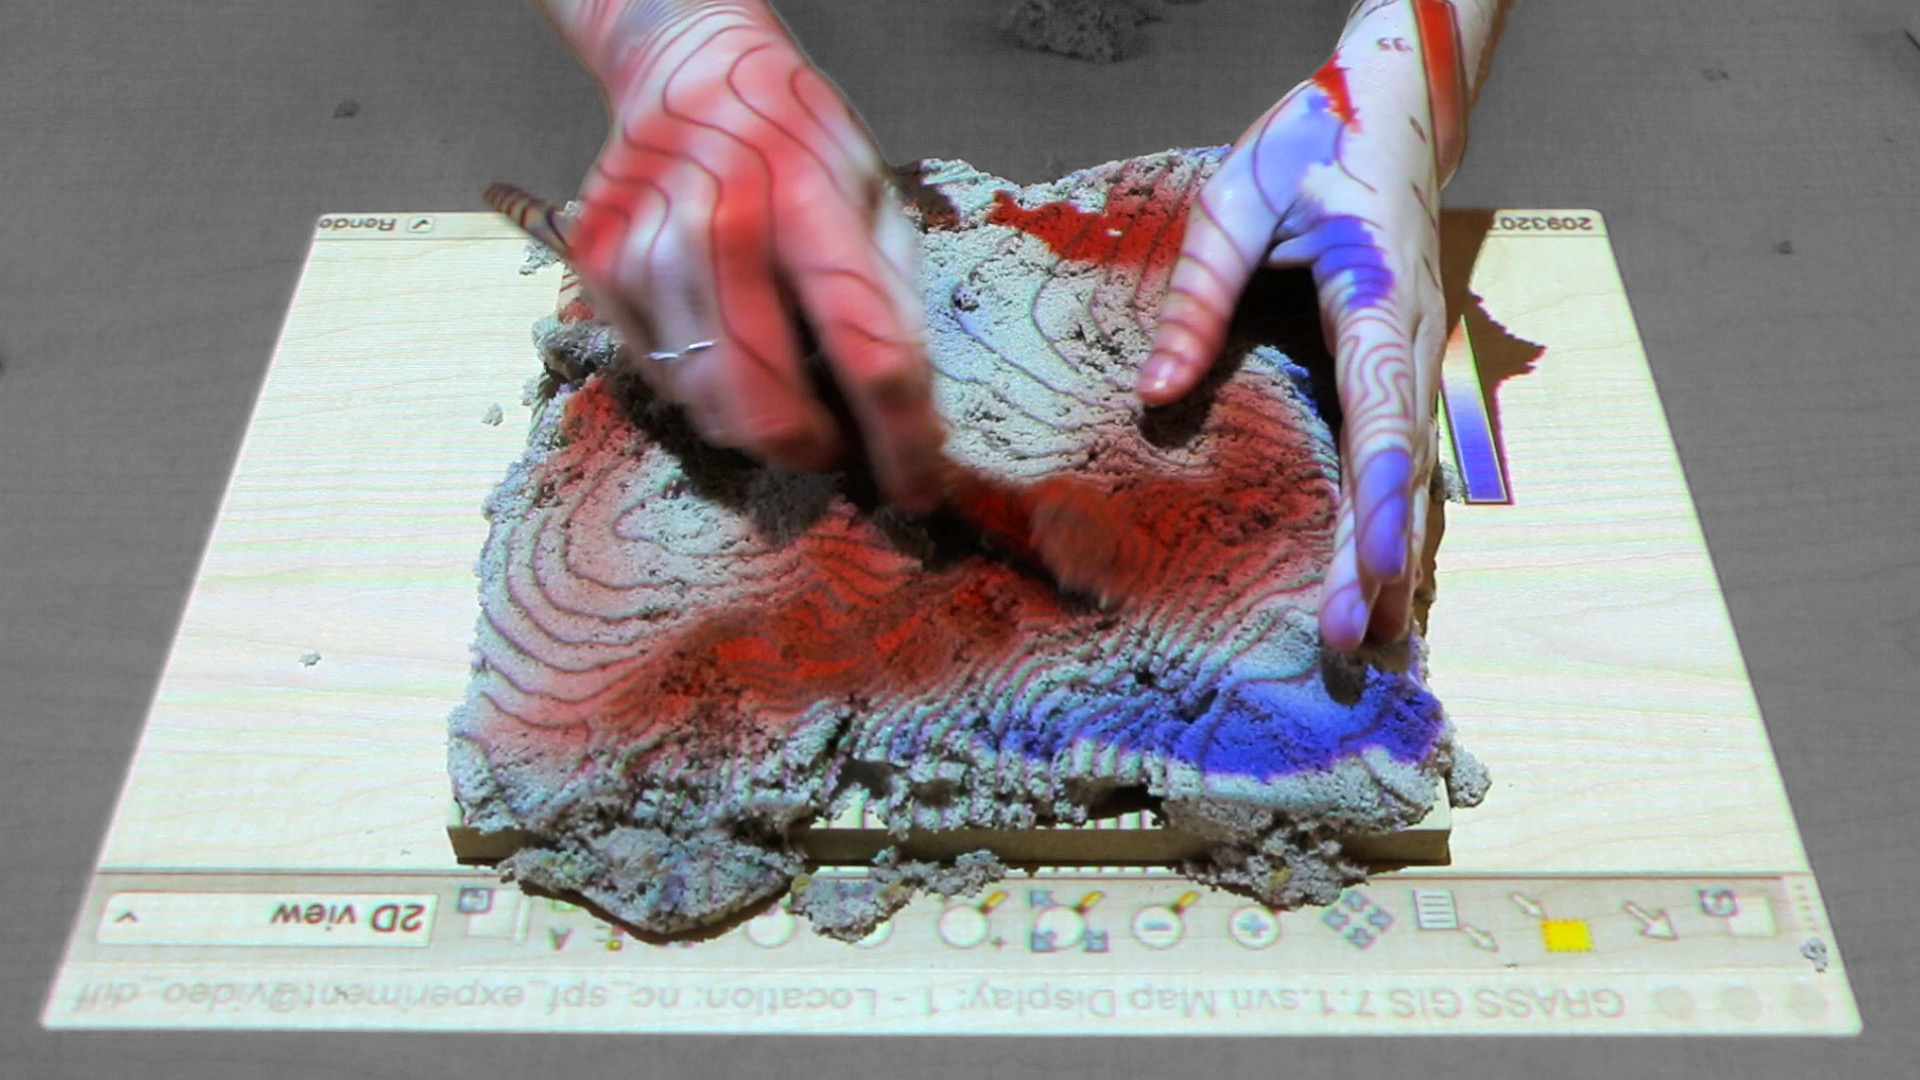
\includegraphics[width=0.49\textwidth]{images/difference/tl_difference_2.jpg}\vspace*{0.2em}
		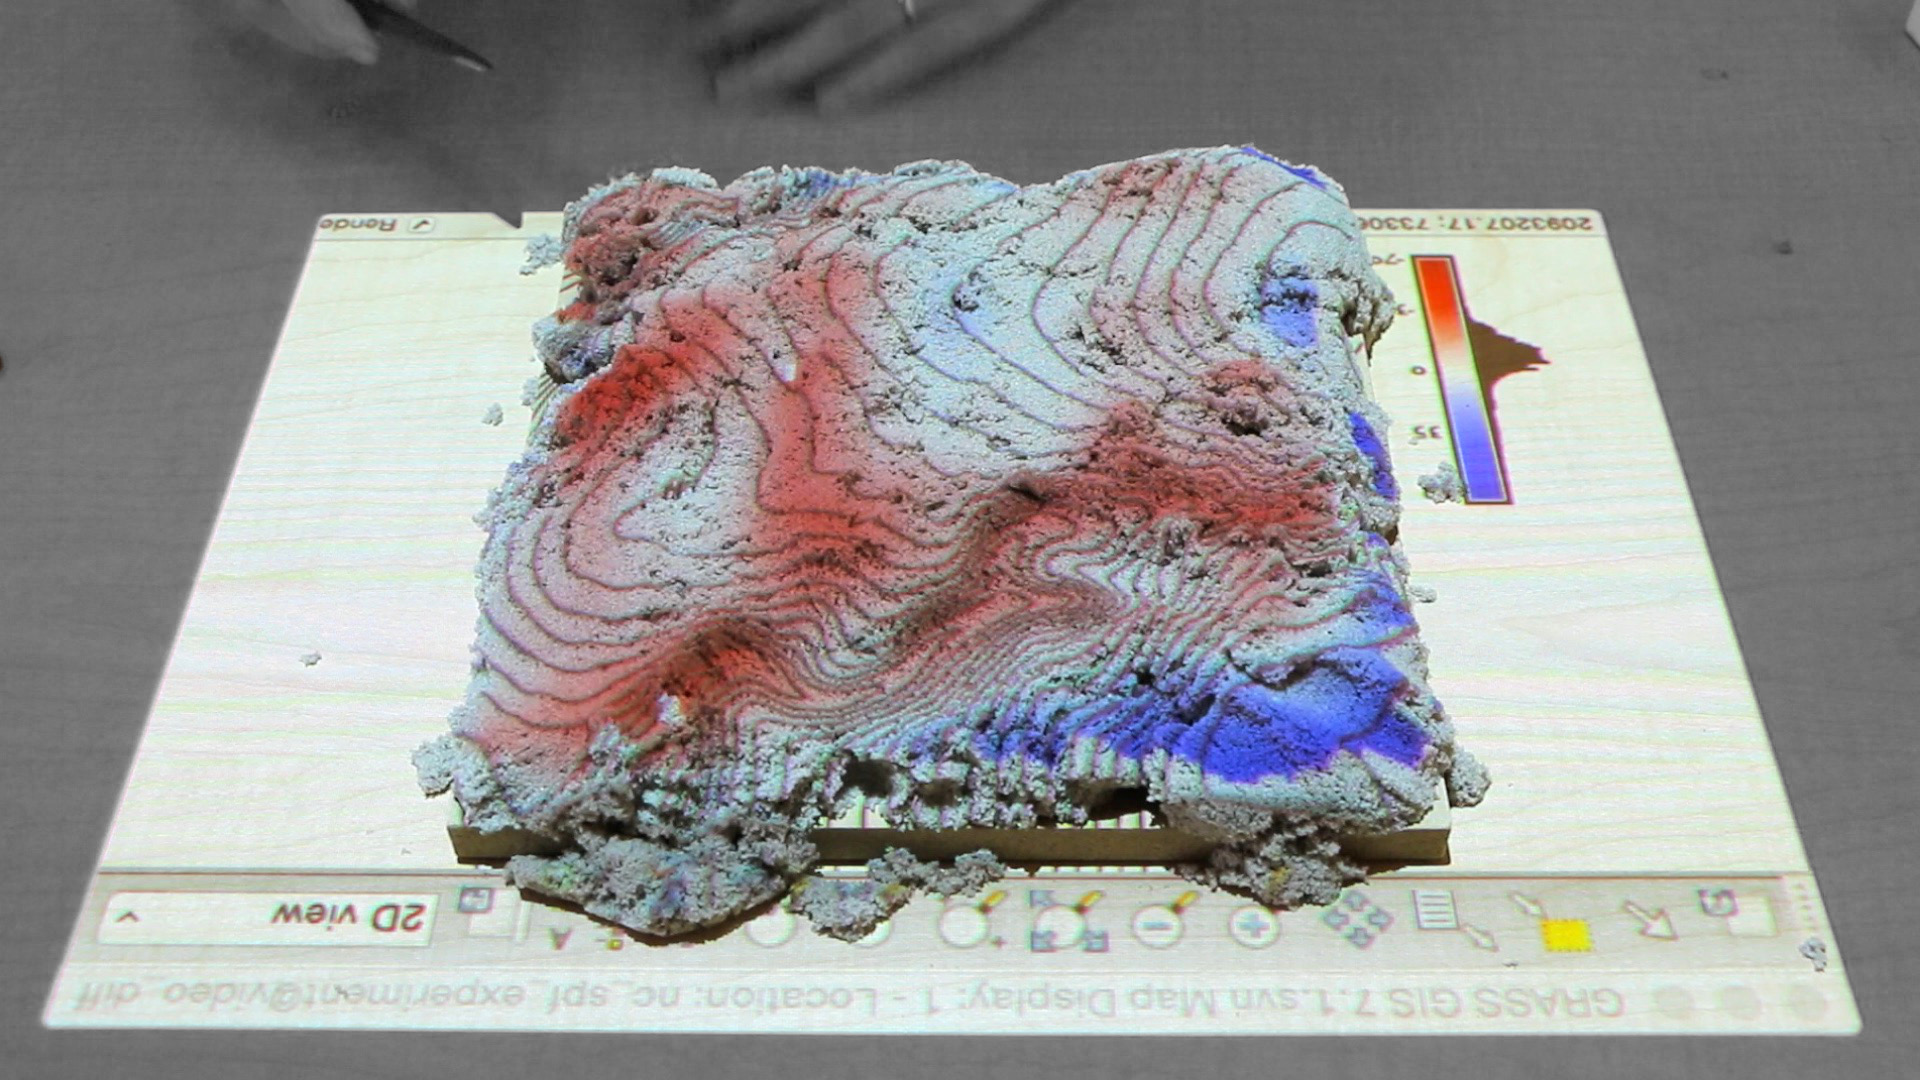
\includegraphics[width=0.49\textwidth]{images/difference/tl_difference_3.jpg}
		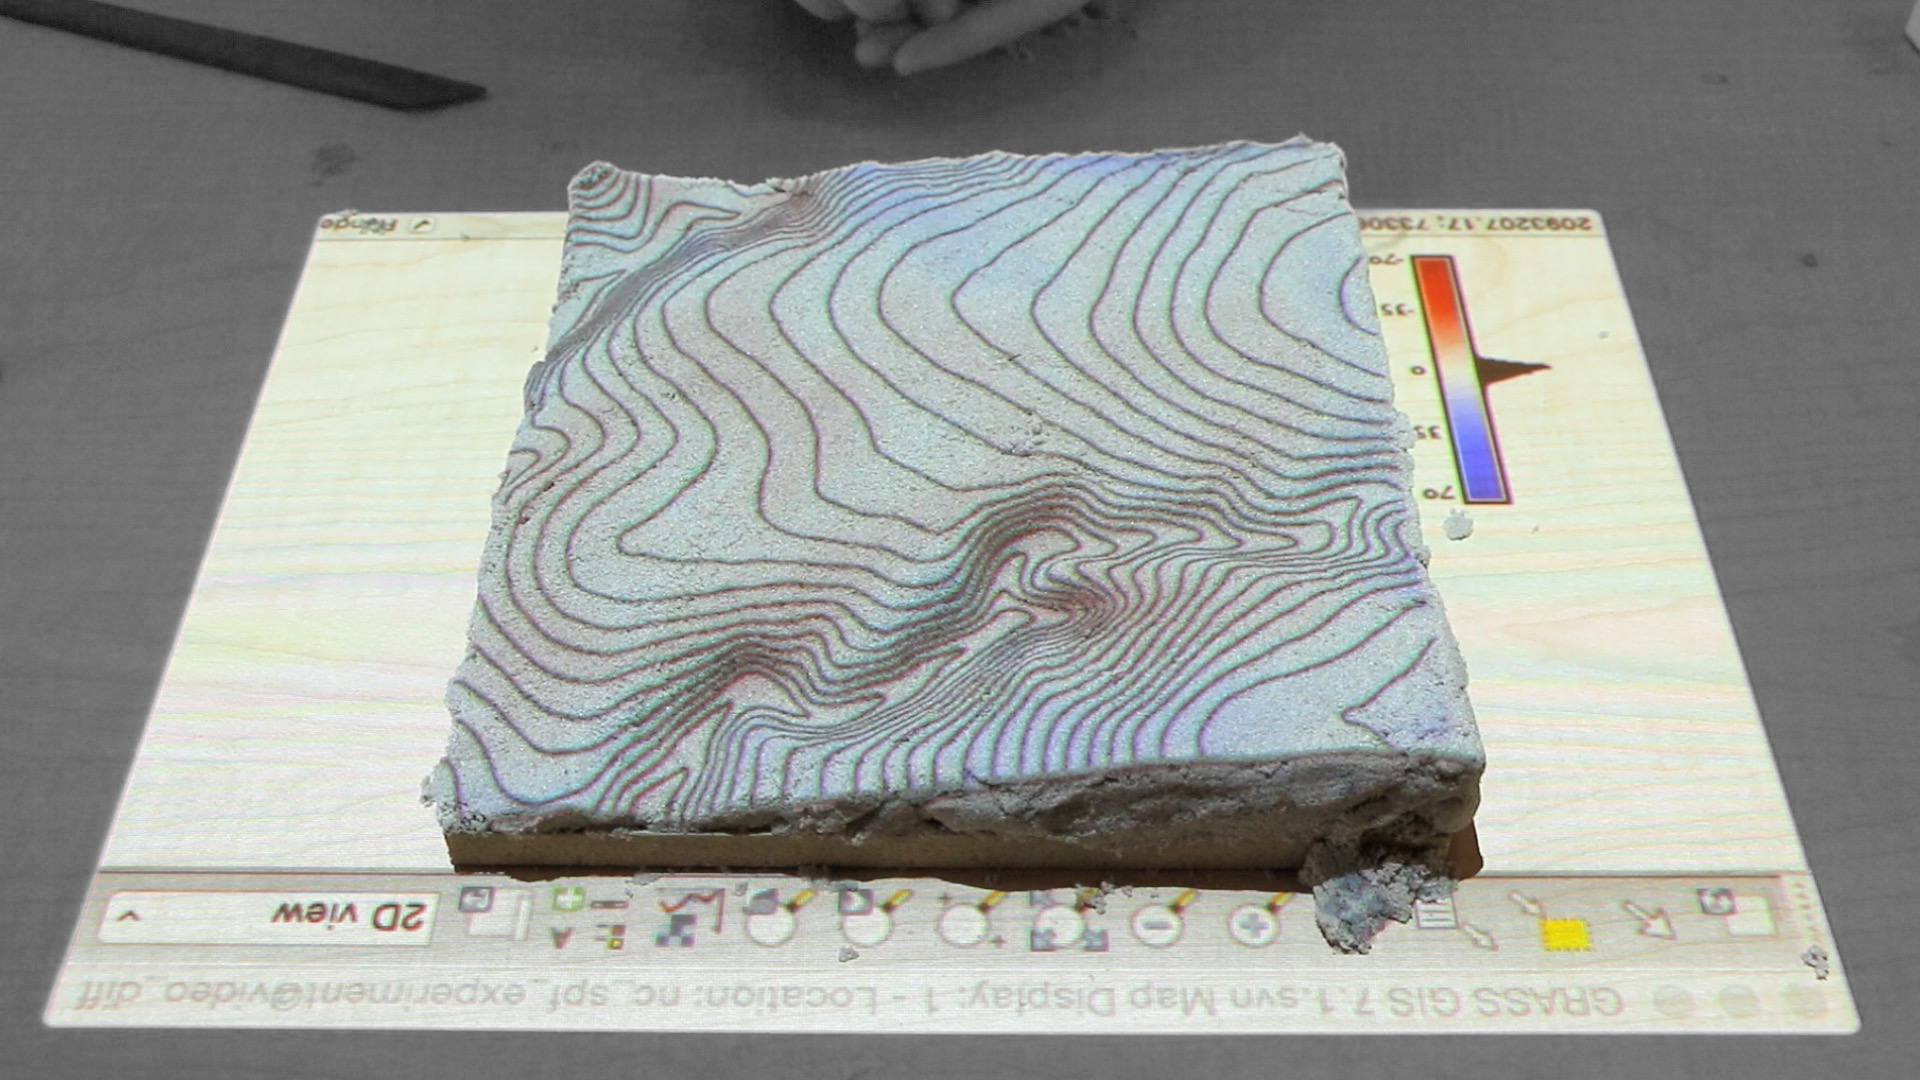
\includegraphics[width=0.49\textwidth]{images/difference/tl_difference_4.jpg}
	\caption{Sculpting a terrain model using Tangible Landscape's difference analytic.
	Blue means add sand and red means remove sand.
	}
	\label{fig:difference_sequence}
\end{center}
\end{figure}

\subsection{Applications}

\begin{figure}
%
\begin{center}
		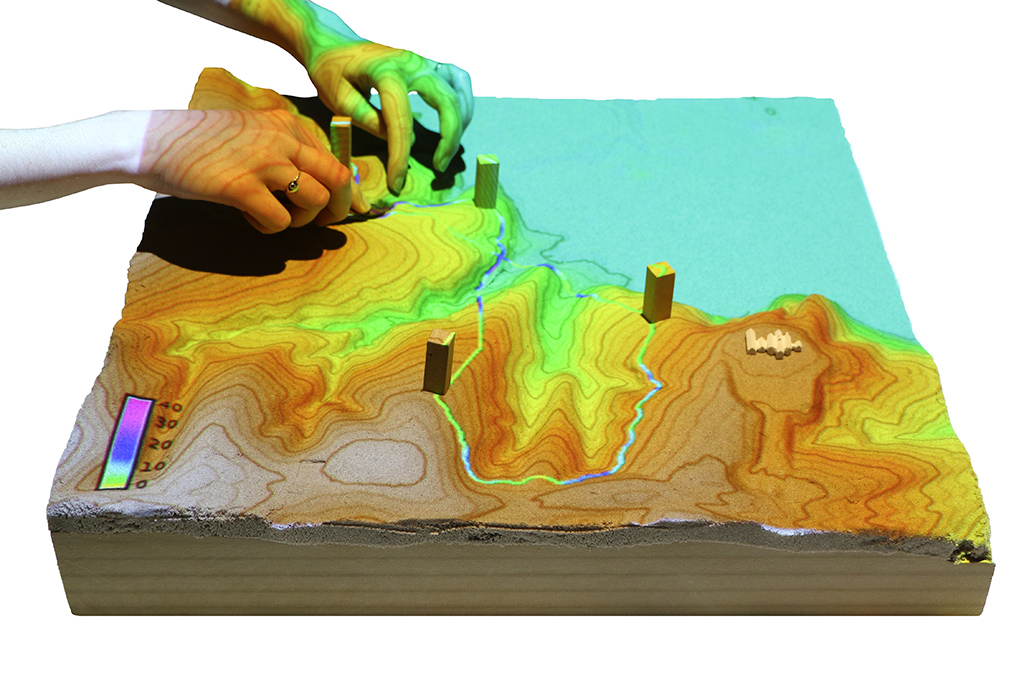
\includegraphics[width=0.49\textwidth]{images/applications/trail_2.jpg}
		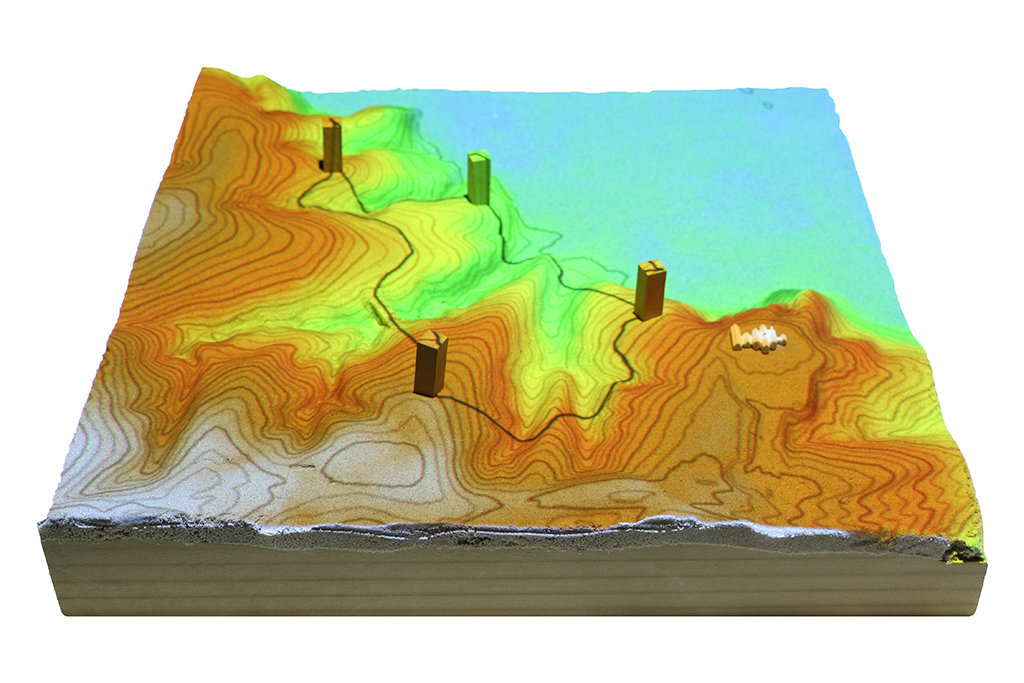
\includegraphics[width=0.49\textwidth]{images/applications/trail_4.jpg}
	\caption{Trail planning with Tangible Landscape. Users create waypoints for a trail by placing markers on the terrain model. The optimal route between the waypoints is automatically computed based on the least cost path and the solution of the traveling salesman problem. Feedback includes the slope along the trail and viewsheds from waypoints. Users can also change the topography and build bridges. Source: \cite{Petrasova2015}.}
	\label{fig:trails}
\end{center}
%
\begin{center}
		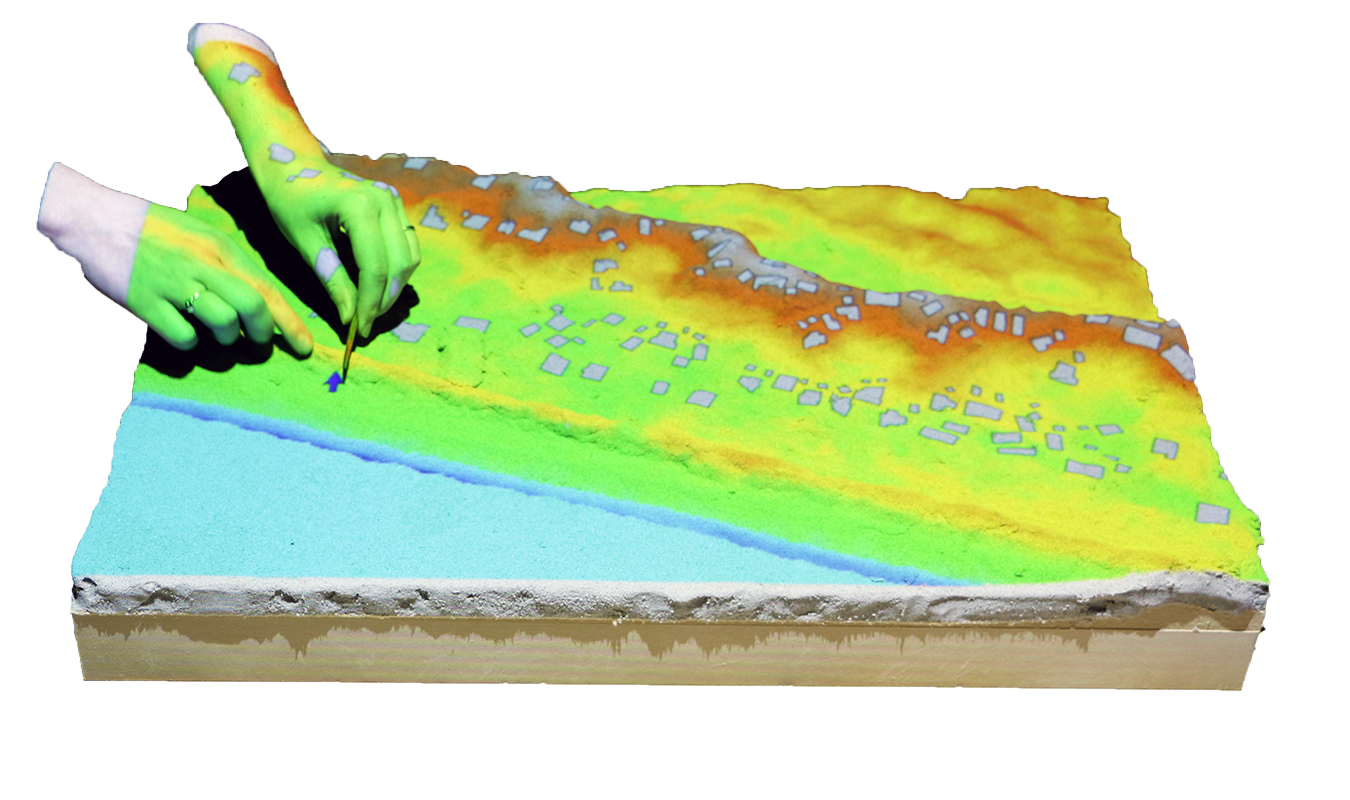
\includegraphics[width=0.49\textwidth]{images/applications/tl_coastal_3s.png}
		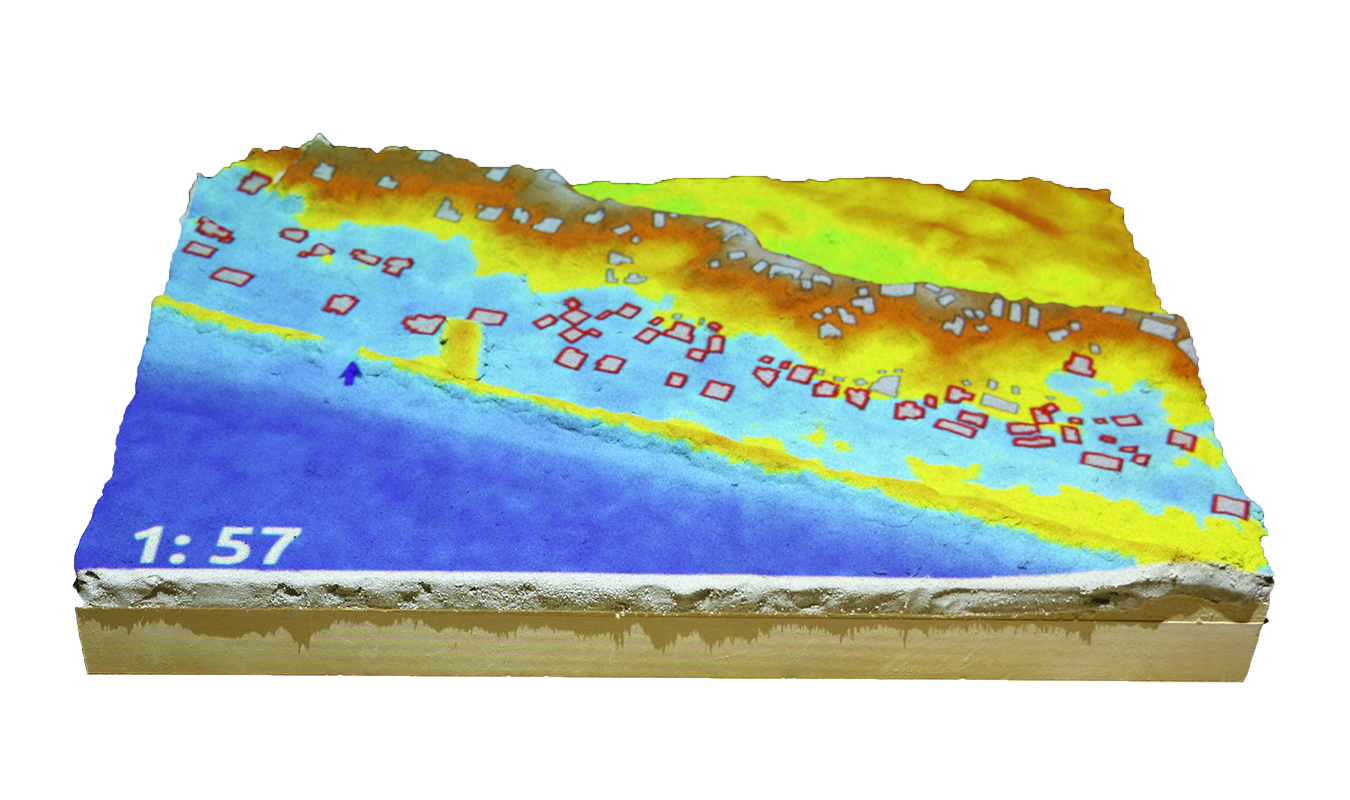
\includegraphics[width=0.49\textwidth]{images/applications/tl_coastal_4s.png}
	\caption{Testing coastal flood defences with Tangible Landscape. Users try to save houses from coastal flooding by building coastal defenses. Given a small handful of polymer-enriched sand -- their budget -- they sculpt new dunes as flood defenses. The foredune is then breached at a random location and simulated storm surge is rerun, flooding any vulnerable houses.}
	\label{fig:coastal}
\end{center}
%
\begin{center}
		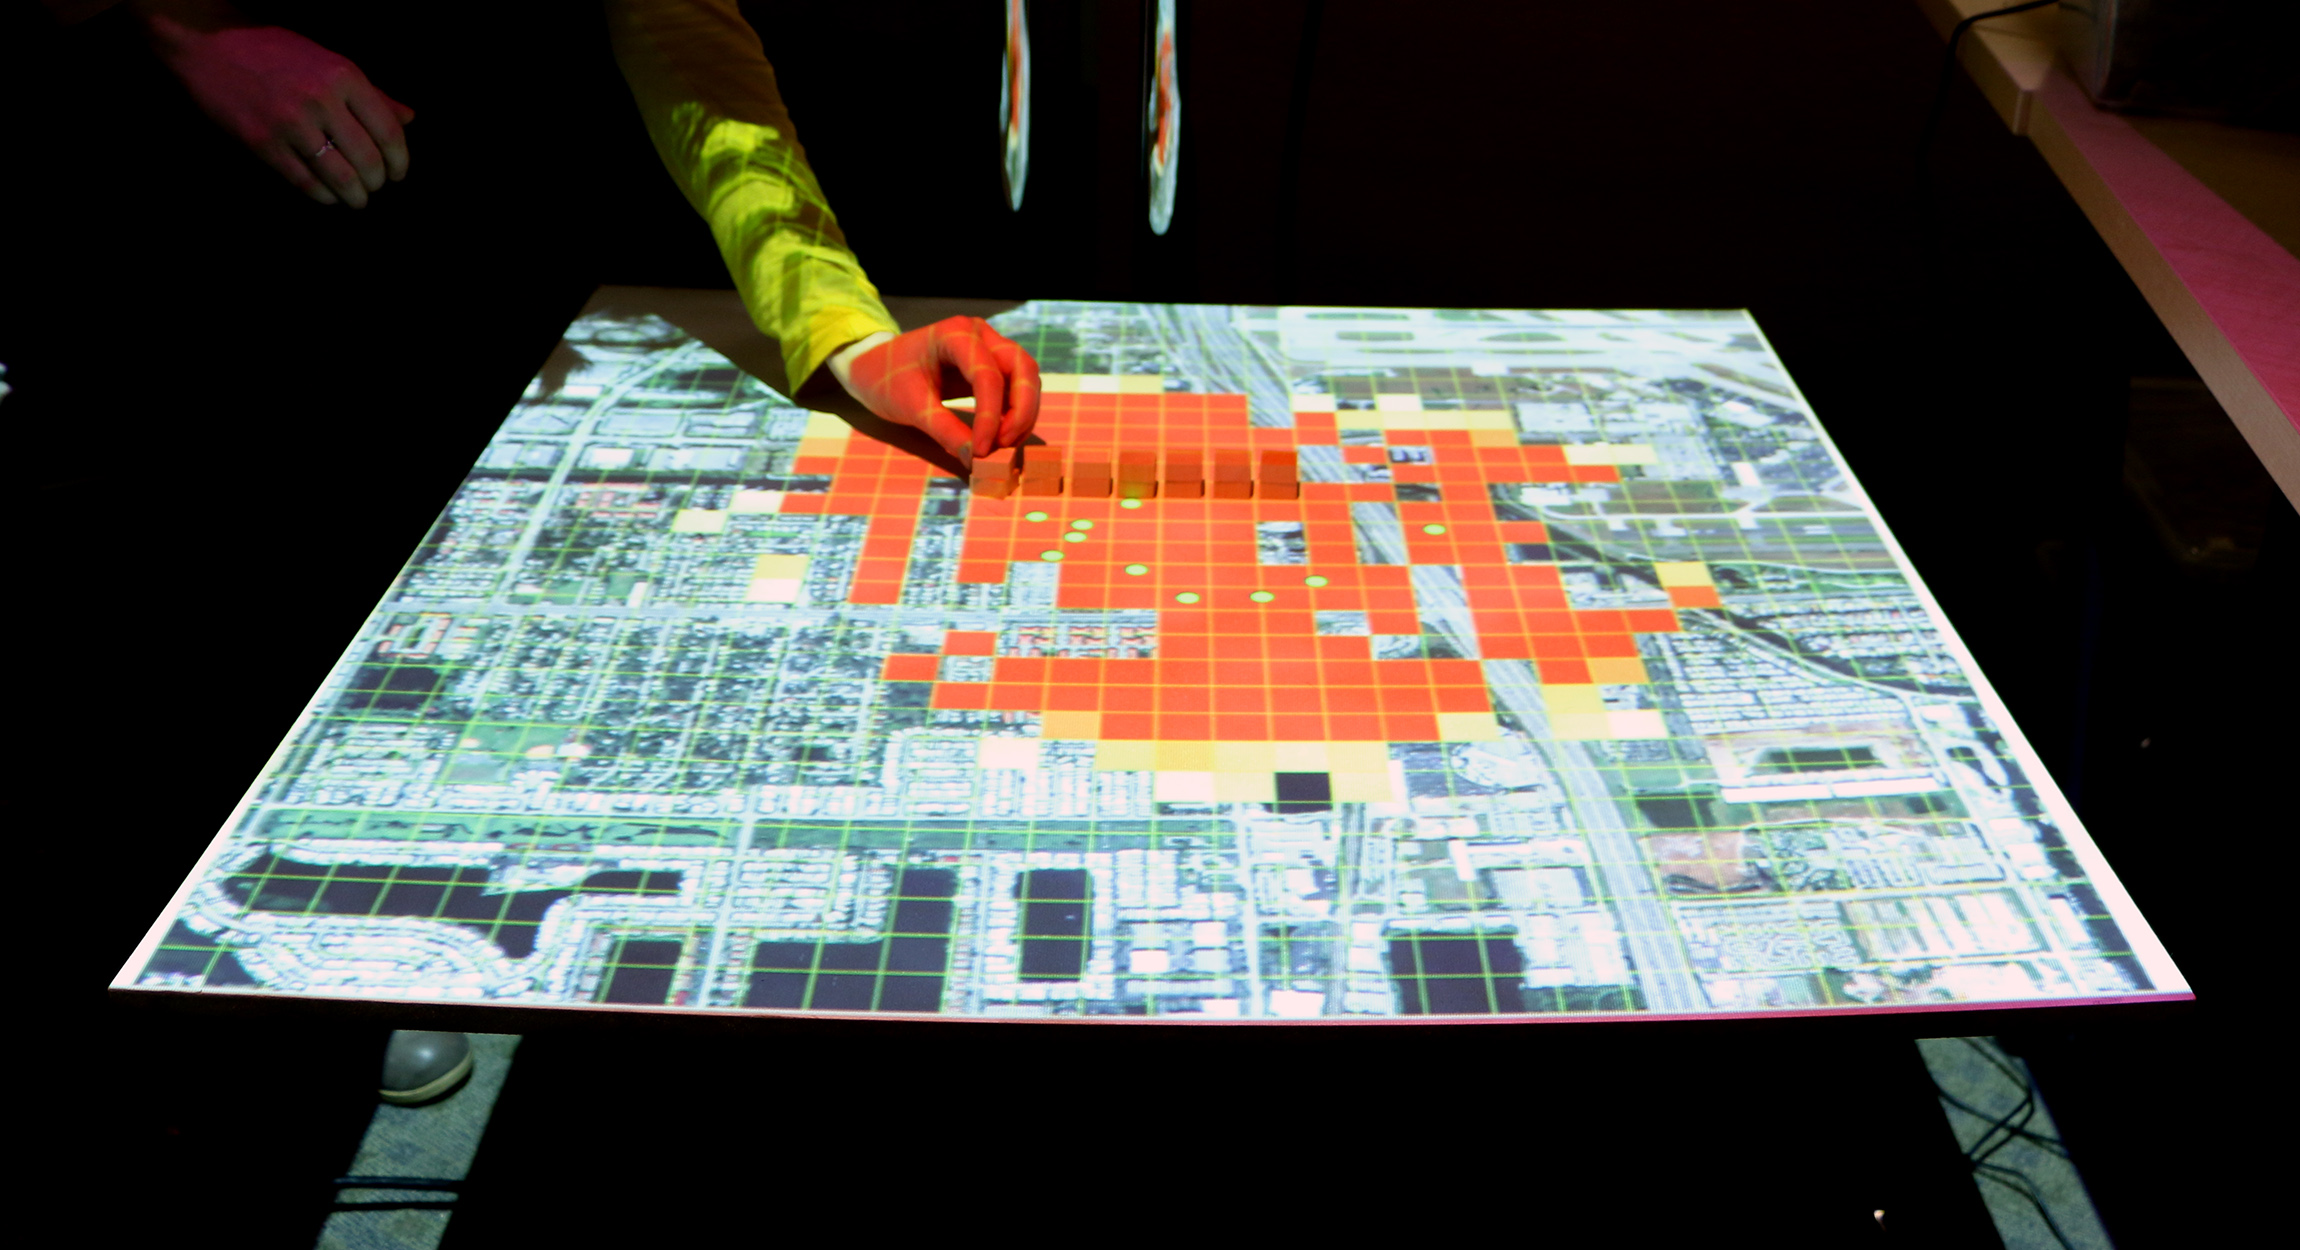
\includegraphics[width=0.49\textwidth]{images/applications/termite_game_2.jpg}
		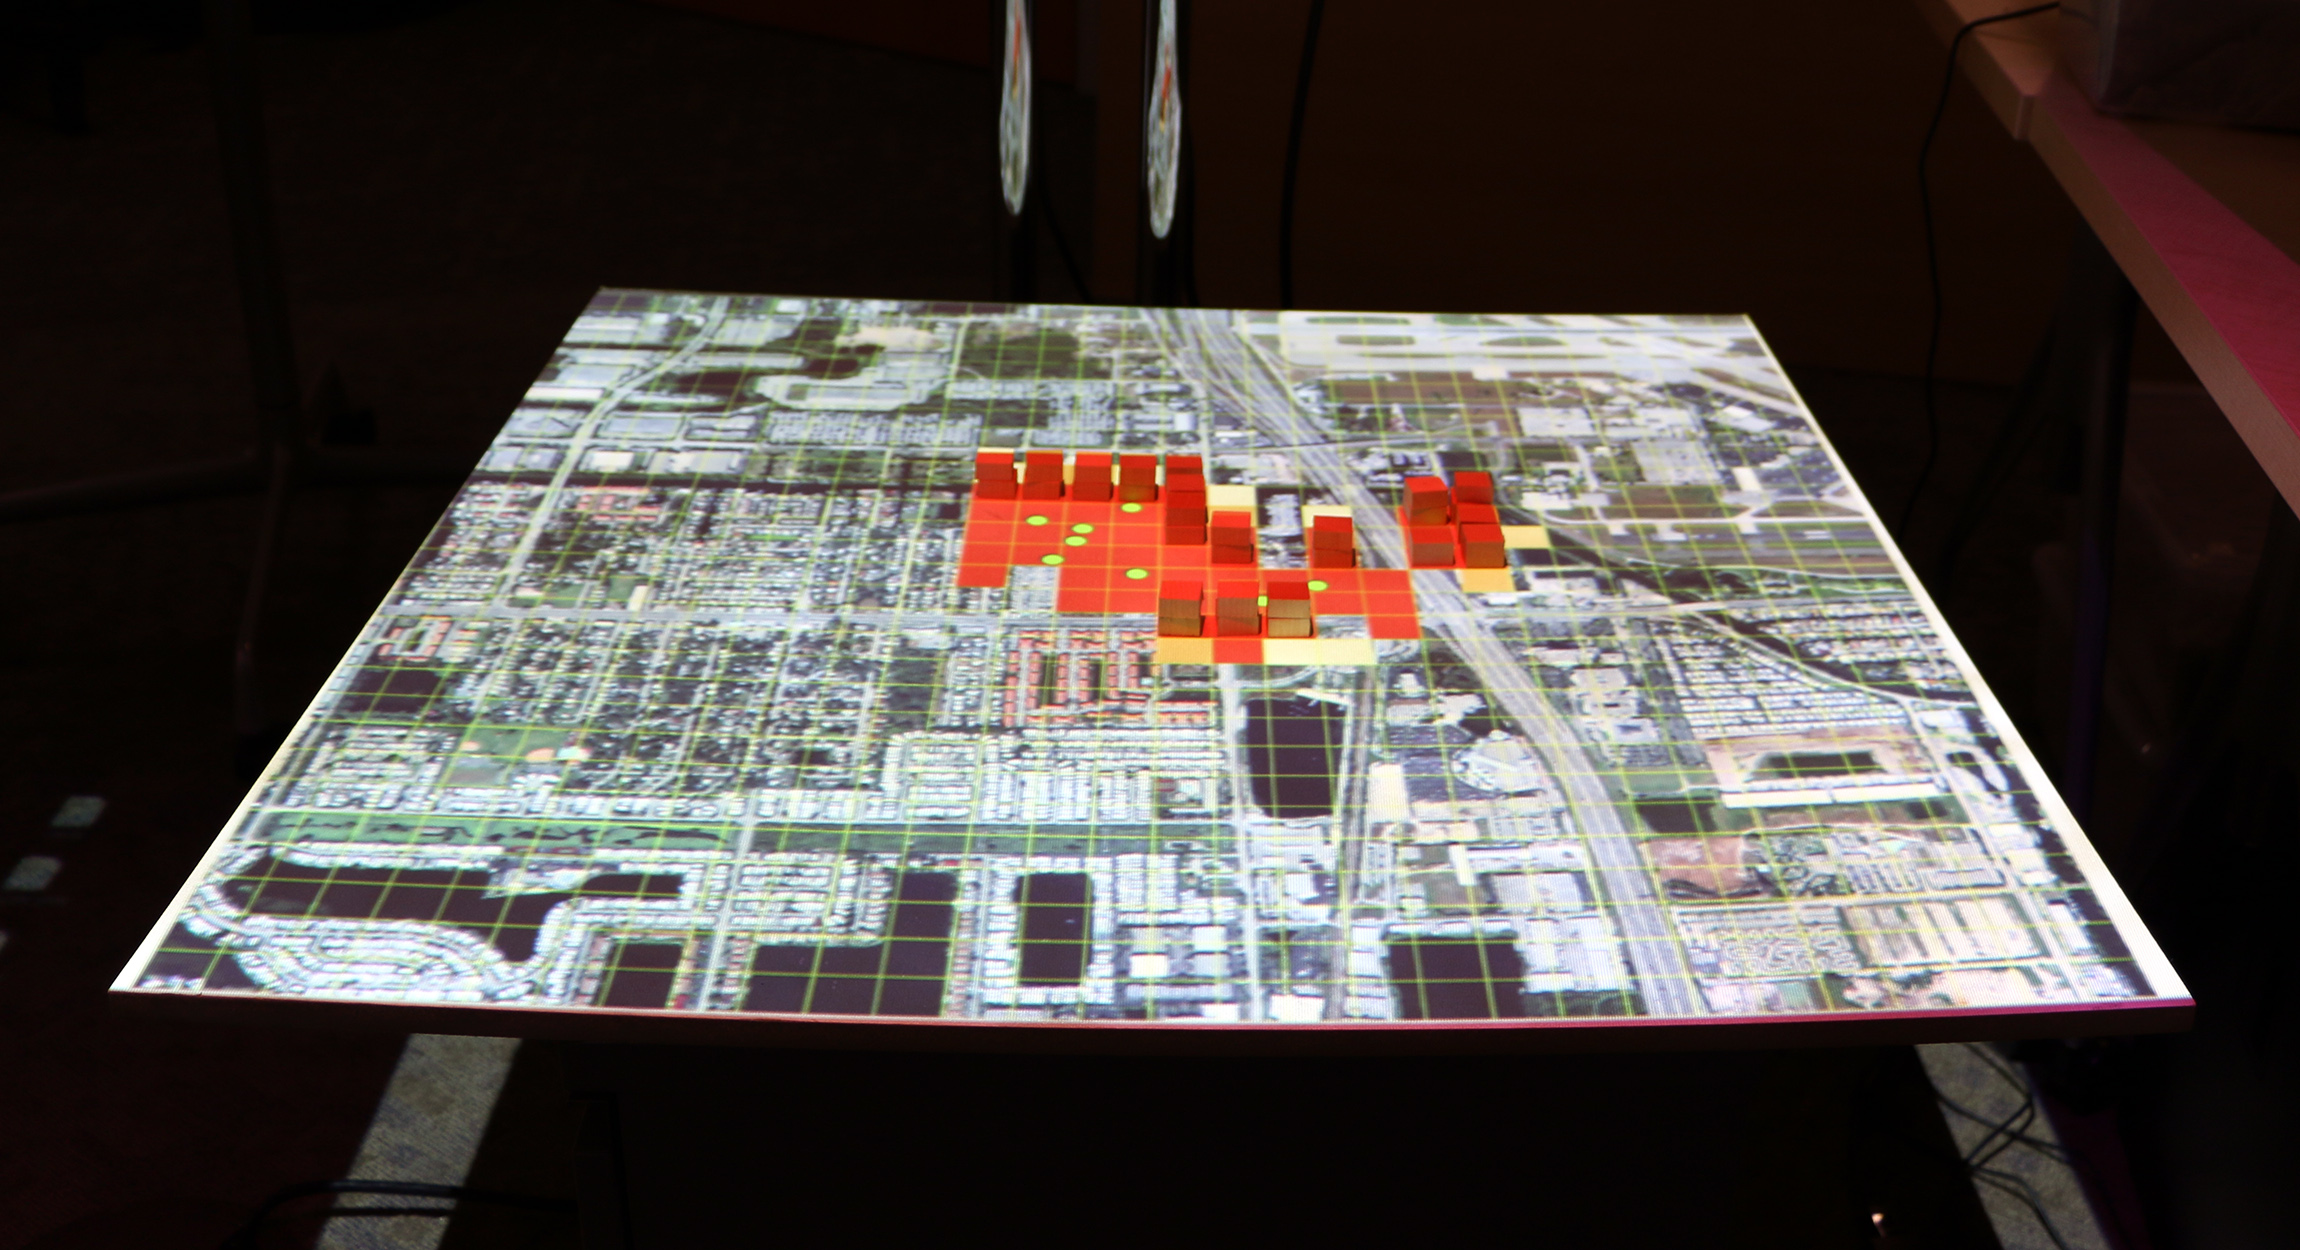
\includegraphics[width=0.49\textwidth]{images/applications/termite_game_3.jpg}
	\caption{Managing the simulated spread of termites through a city with Tangible Landscape by treating city blocks. After watching the simulated spread of termites across the city users place preventative treatments to try to contain the invasion. To treat a city block they place wooden cubes representing preventive treatments on the game board leveraging basic motor skills from childhood play. After they treating 10 blocks the stochastic simulation is rerun so users can see how well they contained the invasion.}
	\label{fig:termites}
\end{center}
%
\end{figure}

Using GRASS GIS's extensive libraries for 
geospatial modeling, analysis, and simulation 
we have developed a wide range of applications for Tangible Landscape 
\cite{Petrasova2015}.
Design and planning applications include
grading, cut and fill analysis, stormwater management, erosion control, 
trail planning (Fig.~\ref{fig:trails}), viewshed analysis, and the assessment of solar potential. 
Scientific applications include
subsurface visualization (Fig.~\ref{fig:subsurface}), urban growth modeling, disease management, and invasive species management (Fig.~\ref{fig:termites}).
Disaster management applications include 
flood control, wildfire management, and coastal change and adaptation (Fig.~\ref{fig:coastal}). 
Educational applications include
spatial training and serious gaming.
%
See Appendix \ref{appendix:videos}
for videos of landscape design (\ref{videos:tl_vr}), viewshed analysis (\ref{videos:viewshed}), wildfire spread (\ref{videos:fire}), and urban growth applications (\ref{videos:urban}).

\section{Coupling experiment}
After a pilot study \cite{Harmon2016b}
we conducted an experiment to study how 
coupling digital and physical models of topography 
mediates 3D spatial performance. 
%
This experiment compared how users performed 
in a terrain modeling task using 
digital 3D modeling with Rhinoceros, 
analog modeling by hand, 
and projection-augmented modeling powered by Tangible Landscape. 
% digital
Digital modeling with a GUI affords precise transformations and
dynamic modes of visualization such as 
3D orbiting, zooming, and ray traced shading,
but is not embodied.
% analog
Theoretically analog modeling -- modeling by hand or with tools -- 
should be embodied, 
affording subconscious, kinaesthetic sensing and manipulation of form. 
By sensing form subconsciously with the body
users should have more cognitive resources for critiquing their work 
and strategizing their next moves. 
% 
Projection-augmented modeling 
couples digital mapping with physical modeling.
Theoretically it should combine affordances of both -- 
enabling enriched visualization and physical sensing and manipulation -- 
to offer more feedback.
While more feedback may help users 
better assess and critique their performance 
so they can strategize their next moves,
too much feedback may be a cognitive overload 
resulting in distraction, frustration, and demotivation. 
Physical sensing and manipulation, however, should offload 
some of this cognitive work onto the body.

\subsection{Methods}
In this experiment 
18 participants tried to accurately model a given study landscape 
digitally, by hand, and with Tangible Landscape. 

% ---------------------------- REVISIONS ---------------------------- 
% 
% Describe participants
% 
% -------------------------------------------------------------------------- 

% EDITOR: 
% Clarify user study details. Why interview some, but not all participants? Is the ordering counter balanced? This could be a big issue if proper study procedures were not taken. Were there learning effects? How did limited time to complete a task play into the results? One would expect a speed/accuracy trade off if time was too short. How proficient in Rhino were your participants? Rhino has a pretty steep learning curve. Please use the suggestions from Reviewer 1 on how to properly describe your study setup and results.

% REFEREE 2: 
% As this study investigates expert users, have the participants used CAD programs before? If so, how frequently do they use it in their work? Are they familiar and comfortable with Rhinoceros, or do they use other CAD software? How many of the participants have worked with GIS models before and have familiarity with contour lines and elevation models? This context is interesting as it relates back to whether the study was aimed at beginners or expert users. In the interviews at page 18, line 41, one participant mentions the long learning curve for digital modeling, which likely influenced her performance.

\paragraph{Participants}
All of the participants 
-- either graduate students, faculty, or professionals 
in landscape architecture or geographic information science -- 
had experience thinking spatially. 
These participants were selected in order to compare 
the performance of novices and experts
in grading (i.e.~earthworking), GIS, and 3D modeling.
Of the 12 graduate students 6 were in the \nth{2} semester of the 
Master of Landscape Architecture program 
at North Carolina State University.
These students were just beginning to learn to read and manipulate contour lines 
in the class Landform, Site Grading, and Development Systems. 
They had no experience with GIS, 3 credit hours of training in digital representation, 
and no experience with Rhinoceros.
The other 6 graduate students were in the \nth{2} semester of the 
Master of Geospatial Information Science and Technology program 
at North Carolina State University.
They had at least 9 credits hours of training in GIS, but 
had no experience with contour maps, digital terrain modeling, or 3D modeling.
The other 6 participants were either landscape architecture faculty 
with professional experience or practicing professionals in landscape architecture 
from around the world. 
Of these 2 were experts in 3D modeling with over 10 years of experience 
using Rhinoceros and similar programs including Maya and 3ds Max. 
These experts felt comfortable and proficient modeling a wide variety of geometries 
and had developed unique, personalized, and highly adaptable workflow 
(see Table~\ref{table:participants}).
%An additional 12 participants took part in the study, 
%but were discarded as they did not complete every task. 

\begin{table}
\tbl{Participants}{
\ra{1.3}
\begin{tabular}{l <{\hspace{1em}} c <{\hspace{1em}} c <{\hspace{1em}} c}
\toprule
Group & No. & GIS training & 3D modeling expertise \\
\midrule
Landscape architecture students & 6 & 0 & 0\\
GIS students & 6 & 6 & 0\\
Academics \& professionals & 6 & 0 & 2\\
\bottomrule
\end{tabular}}
\label{table:participants} 
\end{table}

% ---------------------------- REVISIONS ---------------------------- 
% 
% Order of experiments
% 	Counter balancing
% Time limit
% Rhino
% 	Reasons for choosing
% 		Comparison with Vue
% 	 Design of interaction method
% 	Training
% Physical model for reference
% Interviews
% Videos 
%
% -------------------------------------------------------------------------- 

% REFEREE 1:
% The user studies leave many questions open, regarding the test design and the demographics of the recruited test persons. It sounds like all participants performed the three modeling tasks in the same order (digital, manual, augmented), working with the same desired 3D model. Were there any learning effects? How experienced were the test persons with modeling tasks and/or geographical datasets / maps? At the interview (taken only once at the end of all tests): were the tests persons able to remember details of all the different system variants they had tested? Apparently, only some, selected test persons were interviewed. Which criterion was used for deciding whom to interview and whom not? It looks like there might be a lot of confounding factors associated with the current test design - thereby invalidating the current results.

% REFEREE 2: 
%- As the authors use a within-subjects design, do they take any measures to minimize the practice effect, such as a counterbalance design? This seems especially important for the coupling experiments 1, 2, and 3, which use the same landscape reference model.
%- What version of Rhinoceros is used for the study? I think the paper would benefit from a more detailed description of the Rhino modeling workflow used in the study. Rhino is a popular modeling program and seems like a good choice for a comparison, but I am don’t know if and how it is commonly used in the GIS community. This is not a criticism of the study, just a question to provide more information to help readers without domain expertise in understanding the task better. I did not completely understand the disadvantage of the Vue terrain editor mentioned in the discussion on page 23, as I think that it would produce terrains that are at least as smooth as the point cloud a Kinect would produce. It would definitely be interesting to expand on this point and the lessons learned in the pilot study. Did study participants for instance produce more precise results with Vue compared to Rhinoceros? The reason I think this is important is to address questions that readers may have on how much the study results were influenced by the choice of desktop CAD software. This is of course a very complex and convoluted question that can only partially be answered by any study of this type, but for this very reason it should be addressed with a high level of detail and scrutiny.
%- The system mentions two tools provided for the physical modeling tasks: a 3D scale and a wooden sculpting tool.  Where the subjects advised to use these tools? It would be very interesting to read how many study participants used the tools and if there was a difference in tool use between the analog modeling and the projection augmented modeling task.
%- In Figure 10, a physical model is placed on the table next to the computer screen. Was this model random or did subjects have access to a physical reference model in this condition as well?
%- Why did the study switch to another reference model for the Difference Experiment? It would have been interesting to compare user performance with the conditions in the coupling experiment. As it is presented as a standalone experiment and result, it is hard to evaluate its advantages compared to the other conditions, which would be really interesting given the positive user feedback.
%- How was the time constraint of 10 minutes chosen? Did this condition create time pressure for study participants or were most of them done and satisfied with their models at the end of each time slot? If the participants were given 20 minutes instead of 10, would they have refined the models further in all these conditions? The reason I am interested in this question is because I wonder if participants would have refined the Rhinoceros models further to be less abstract and eventually produced a more precise model than what they could have achieved with the Tangible Landscape. If that were the case, the study would indicate that a 3D modeling TUI can outperform GUI for quick modeling tasks.

\paragraph{Experimental design}
% tasks
Participants were given three tasks -- 
to digitally sculpt a model a landscape using the 3D modeling program Rhinoceros, 
to hand sculpt a model of a landscape in polymer-enriched sand,
and to sculpt a model of a landscape using Tangible Landscape.
% time limit 
They had 10 minutes to complete each task. 
The time limit was calibrated based on 
the time it took the research team 
to comfortably complete each task. 
% counterbalancing / order of tasks
The modeling tasks were reordered for each participant
to partially account for learning and fatigue
by counterbalancing the experiment using a Latin square design.
% assessment
Participants were asked to model the same landscape for each task 
so that their performance could be quantitatively assessed 
using spatial modeling, statistics, analysis, and simulation.
Their modeling processes were qualitatively assessed 
through direct observation
supported by photographic and video documentation. 
% 
After completing the tasks
the academics and professionals 
were interviewed. 
We intended to conduct semi-structured interviews 
with all of the participants, but
the students were too tired by the end of the experiment. 
%
Psychometric tests were not used
to assess spatial ability because
these do not address 
geographic scales,
spatial relations,
domain-specific knowledge and abilities 
\cite{Lee2009,Bednarz2011,Wakabayashi2011},
or embodied cognitive ability. 
%
See Appendix 
\ref{appendix:procedure} for instructions for running the experiment
and Appendix 
\ref{appendix:guidelines} for semi-structured interview guidelines. 

% study landscape
We used a region of Lake Raleigh Woods in Raleigh, North Carolina 
as the study landscape for this experiment. 
A real landscape was used because computer generated landscapes 
often look surreal and may lack distinct landforms and clearly defined streams. 
This study region has distinctive, 
clearly defined landforms -- a stream valley flanked by a ridge and sloping towards the lake.
%(see Table~\ref{table:coupling_experiment}). 
The digital elevation model for this region was derived from a 2013 airborne lidar survey 
using the regularized spline with tension interpolation method \cite{Mitasova2005}. 
% physical reference models
We CNC routed a model of the study landscape in Baltic birch 
using 2 parallel finish cuts 
with a 3.175 mm diameter ball-nose bit
with a 1.27 mm stepover. 
Participants were given this model 
at the beginning of the experiment
to use as a reference during each task.

\begin{figure}
\begin{center}
	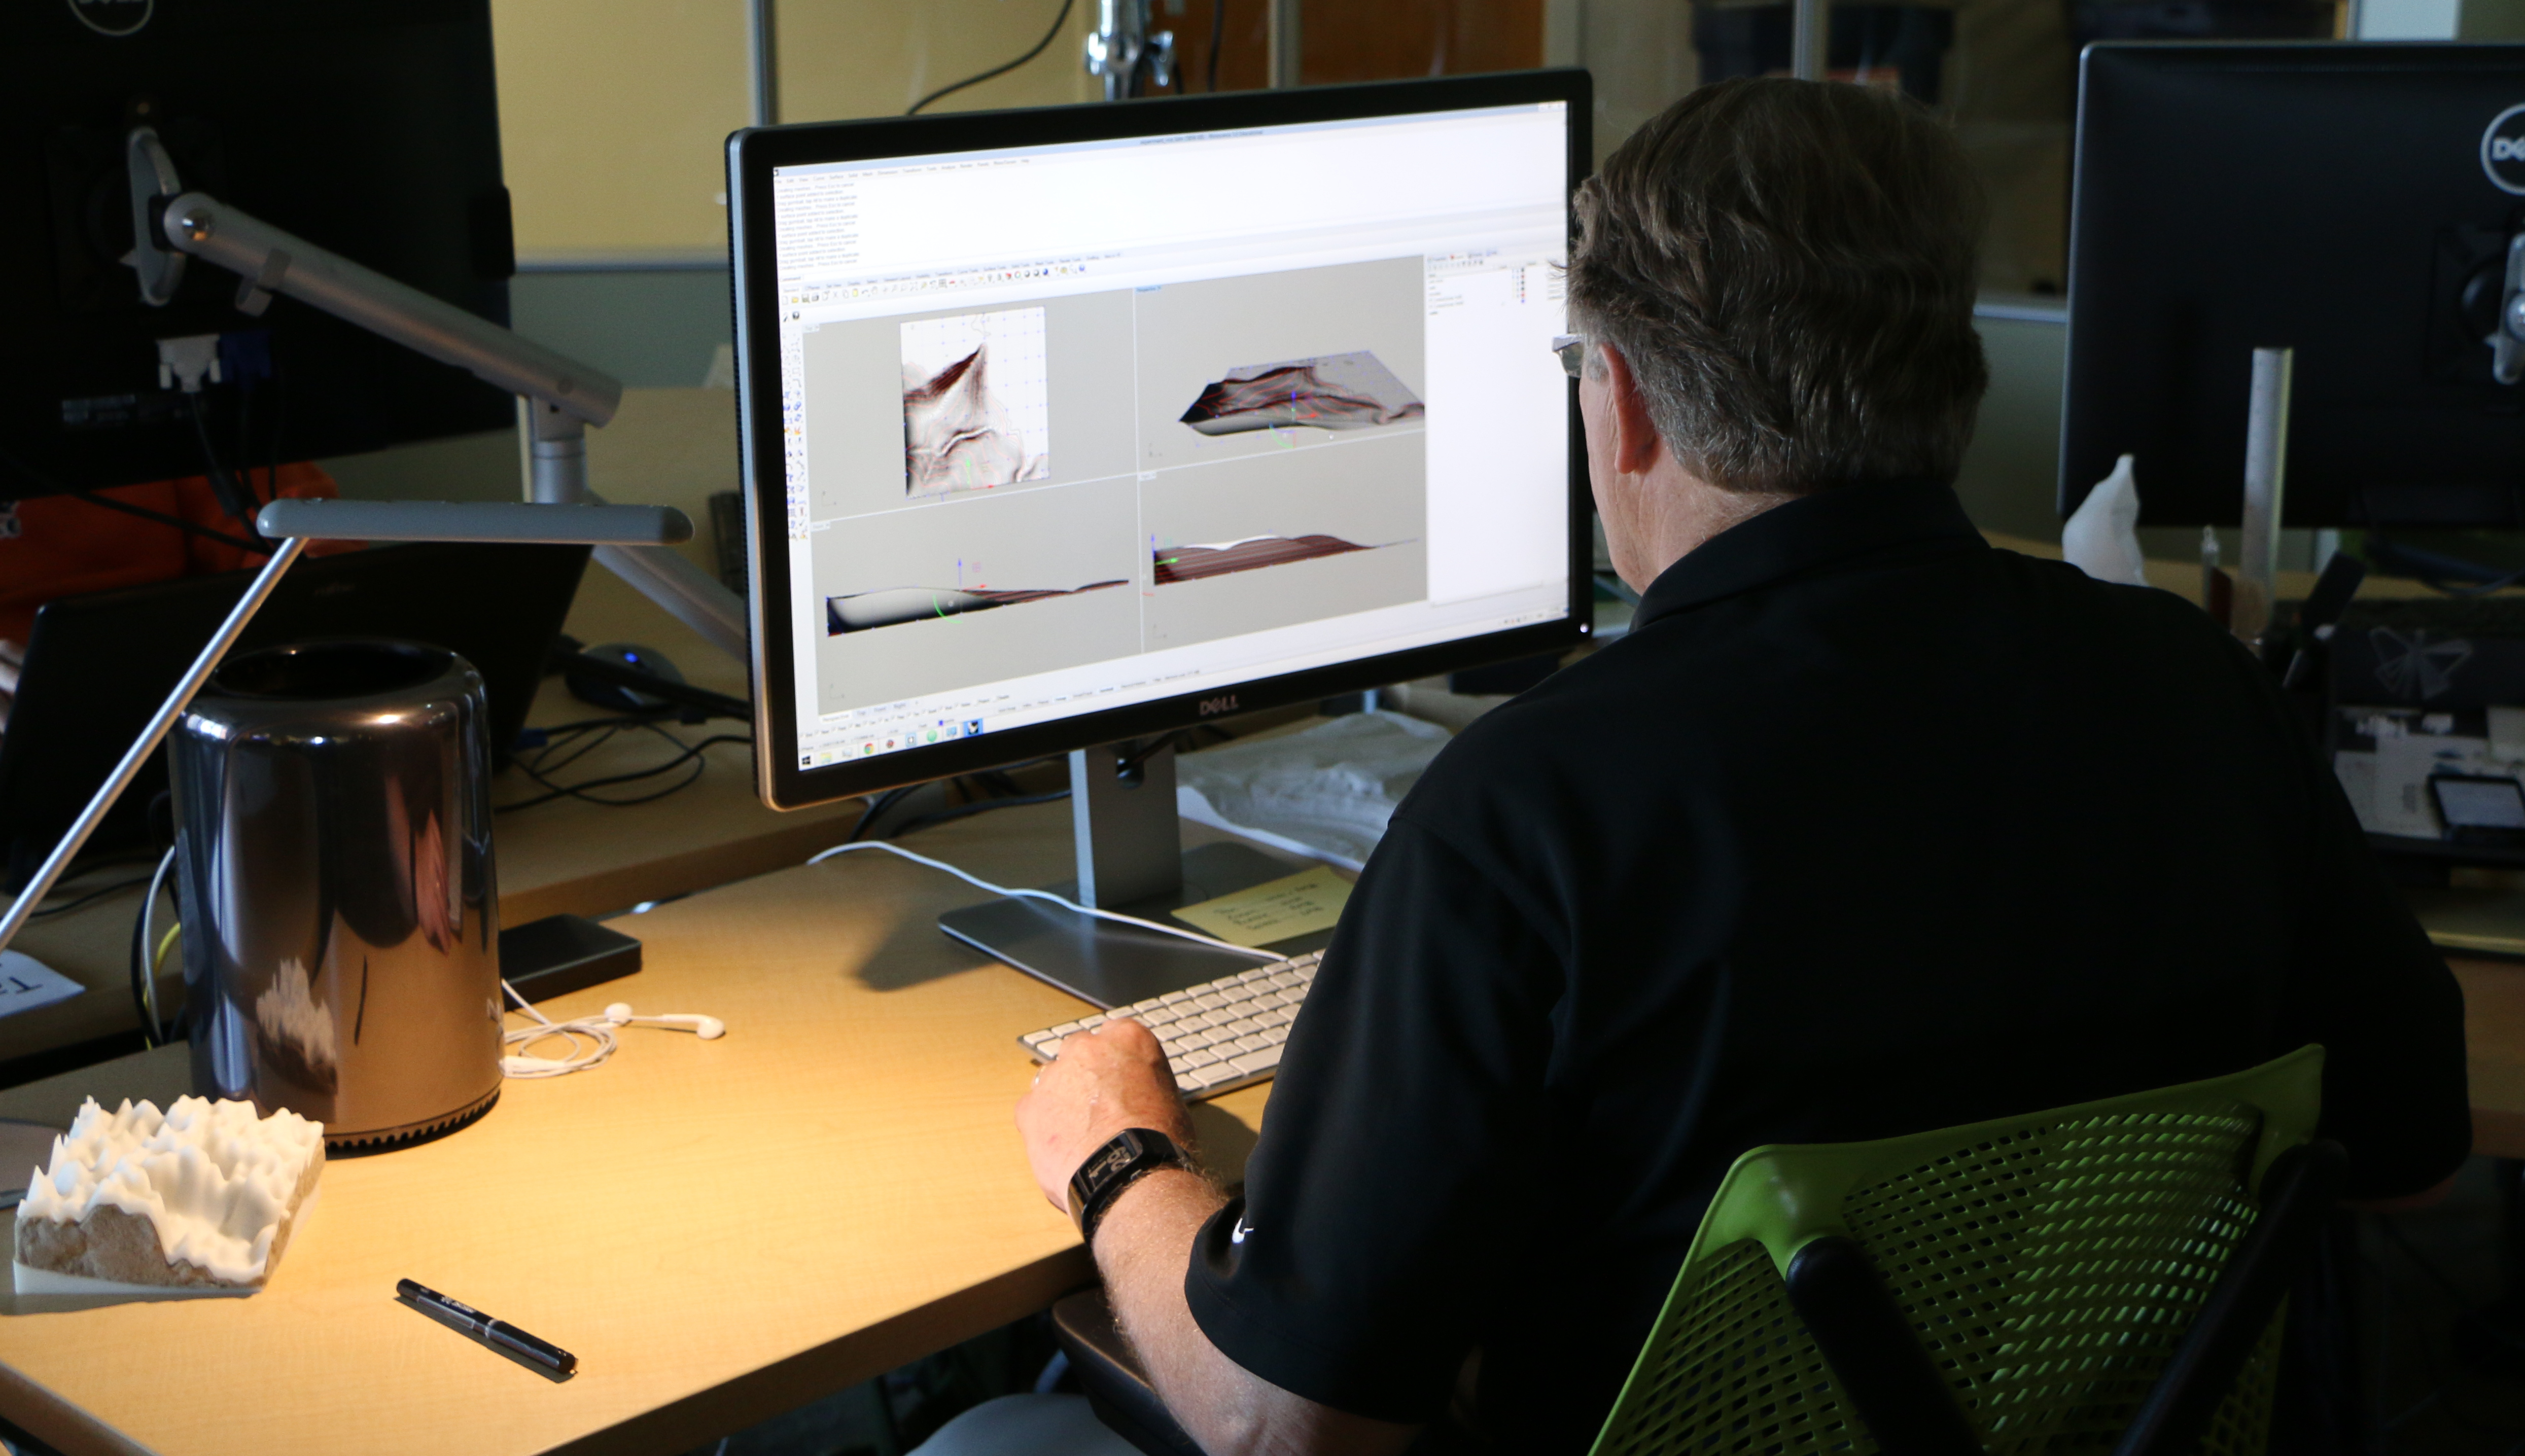
\includegraphics[height=108px]{images/experiments/art_rhino.jpg}
	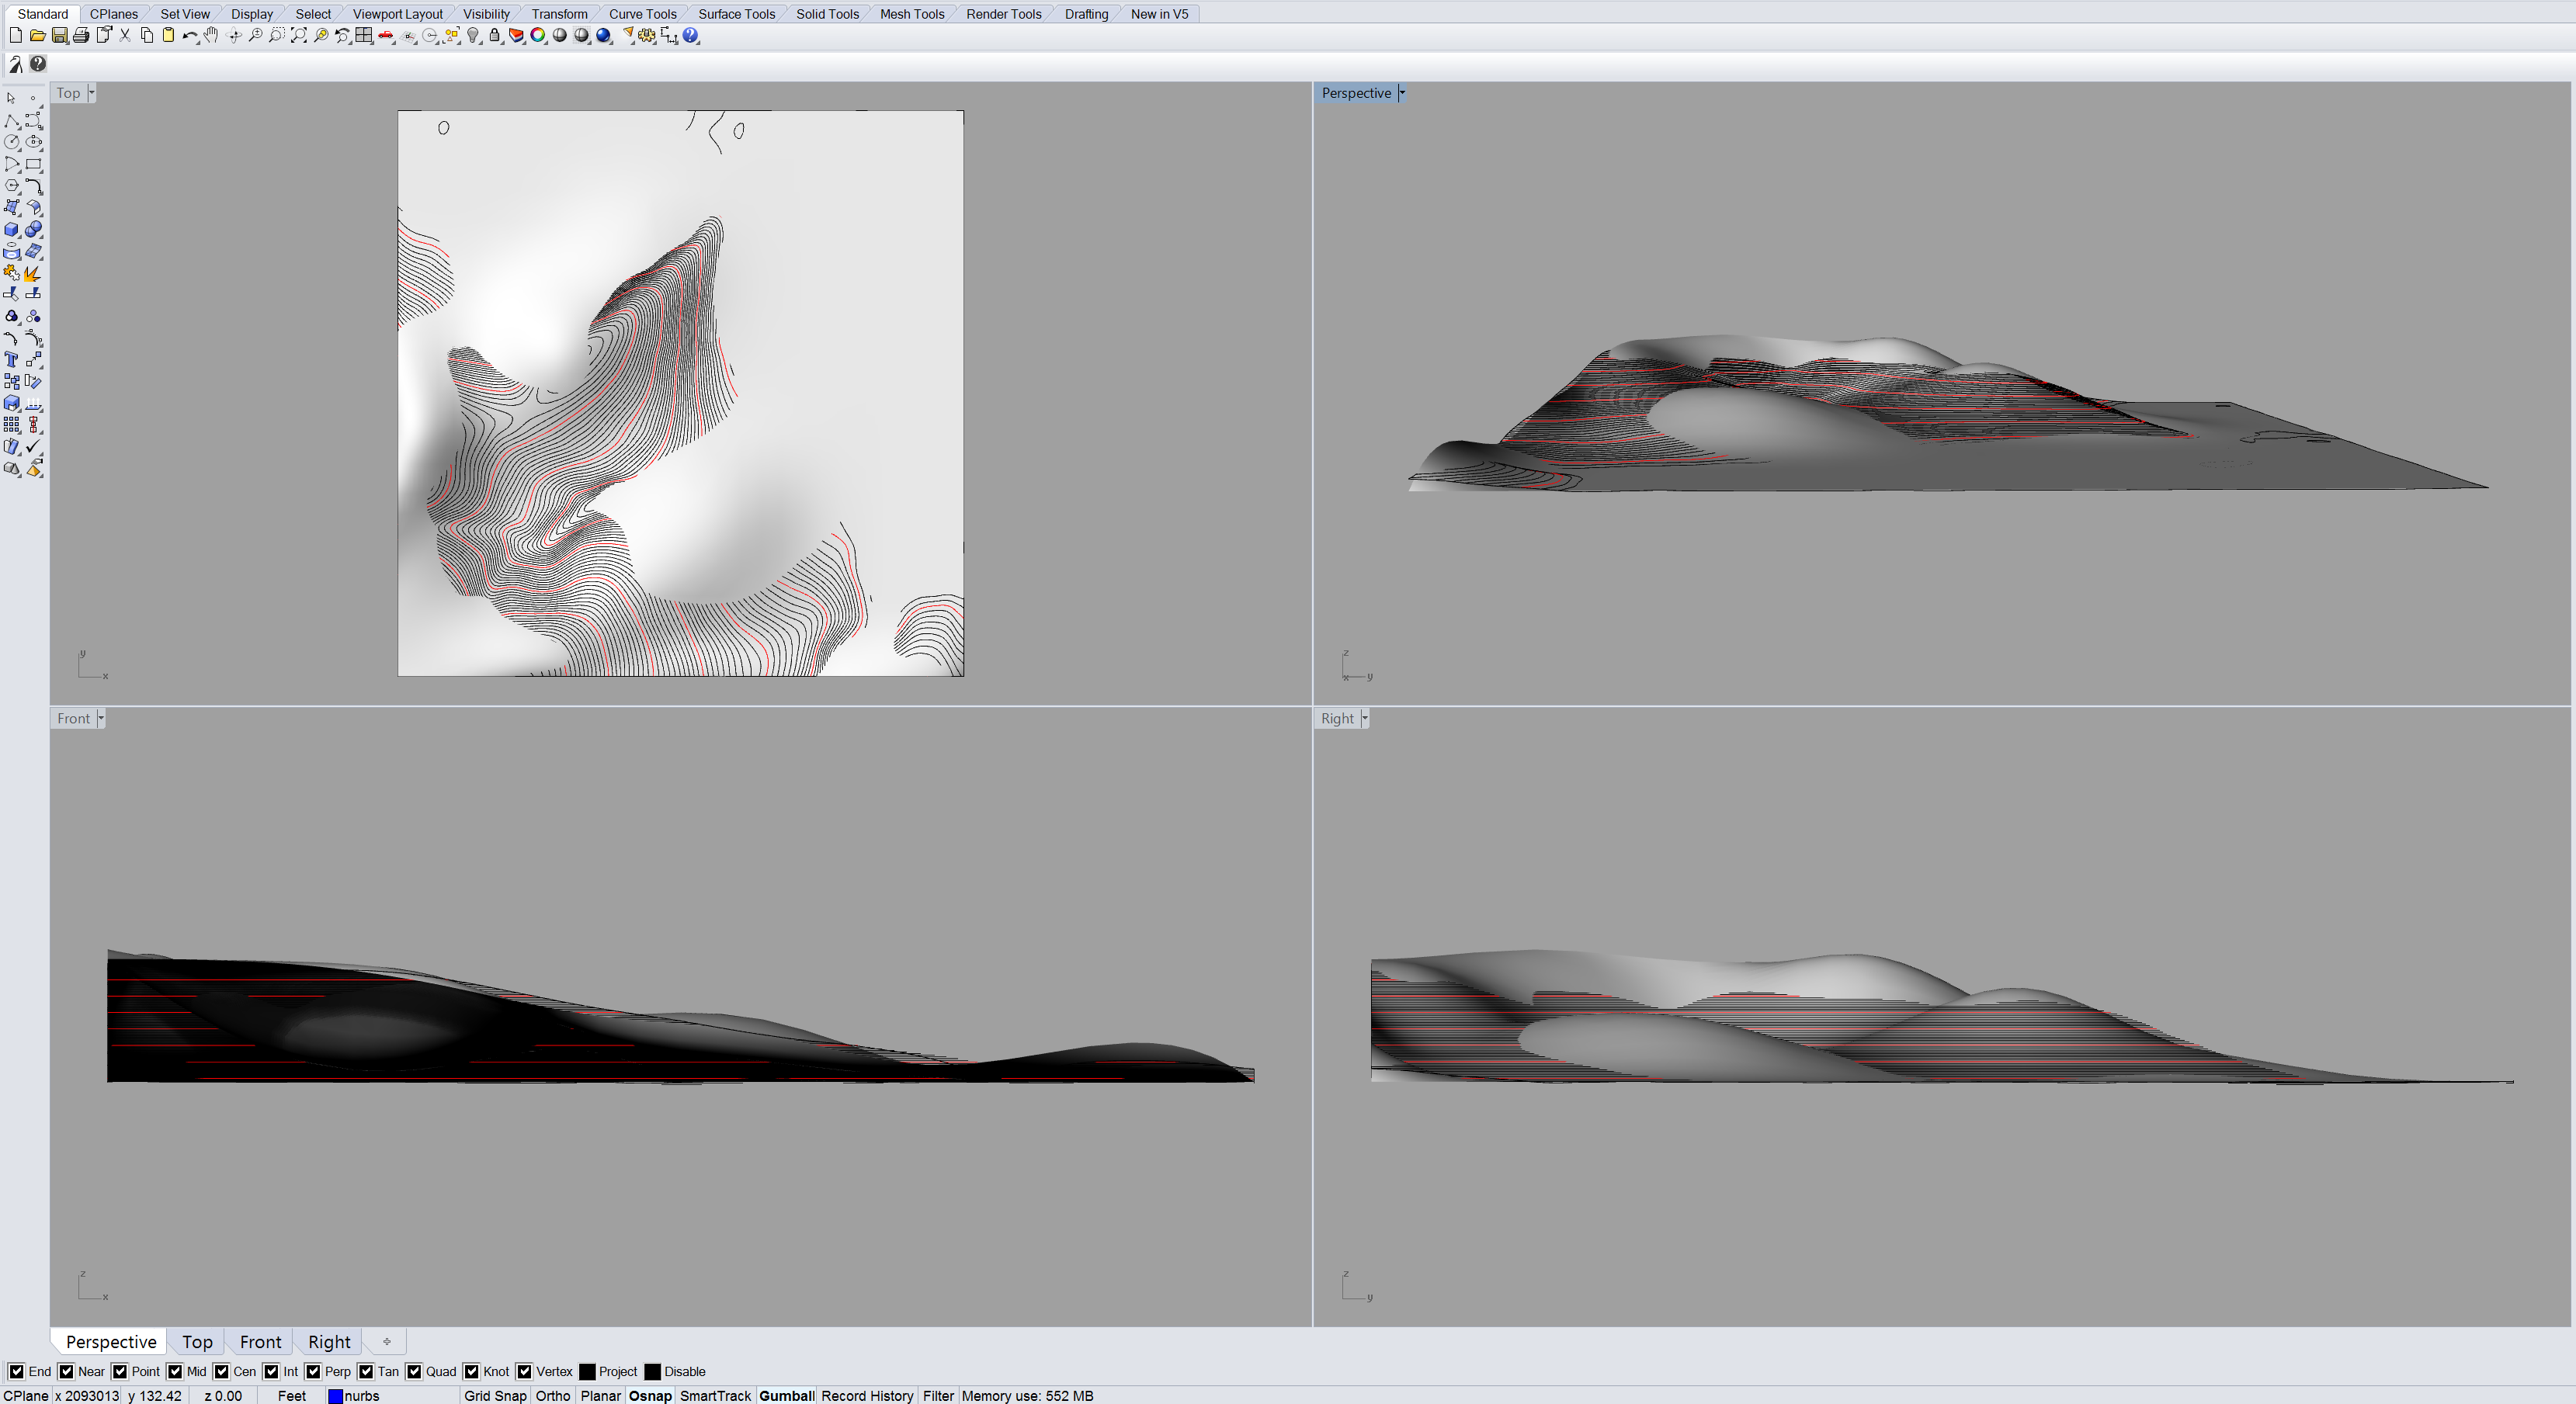
\includegraphics[height=108px]{images/experiments/rhino.png}
	\caption{Coupling experiment - digital modeling:
	A participant digitally sculpts the study landscape in Rhinoceros
	using 3D contours as guides.}
	\label{fig:rhino}
	%
	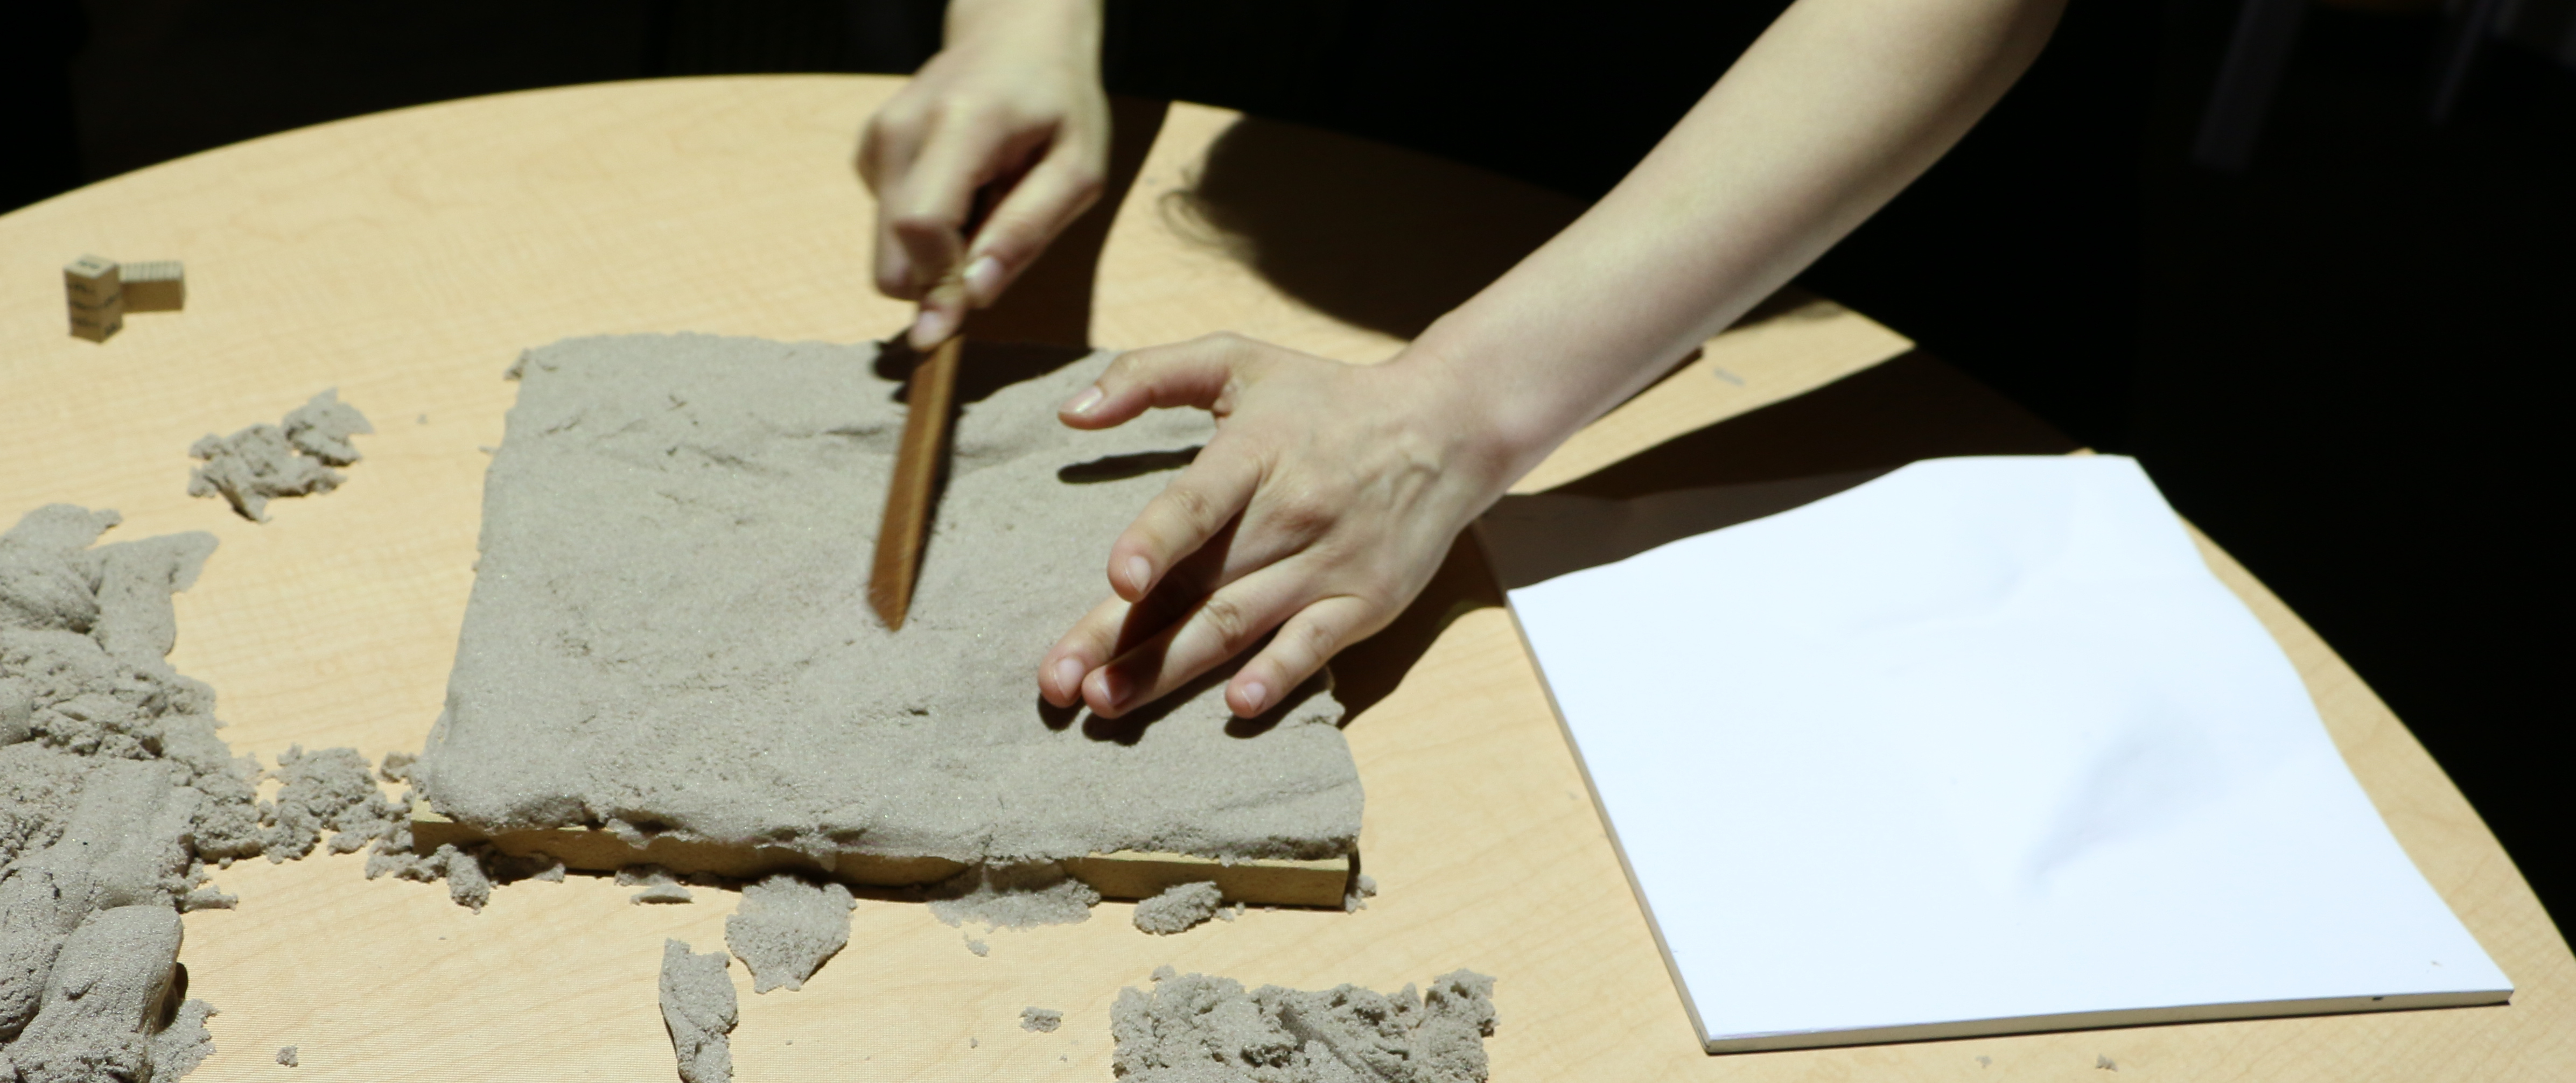
\includegraphics[width=\textwidth]{images/experiments/connie_analog_1.jpg}
	\caption{Coupling experiment - analog modeling by hand:
	A participant sculpts the study landscape by hand
	using a physical model as a reference.}
	\label{fig:analog}
	%
	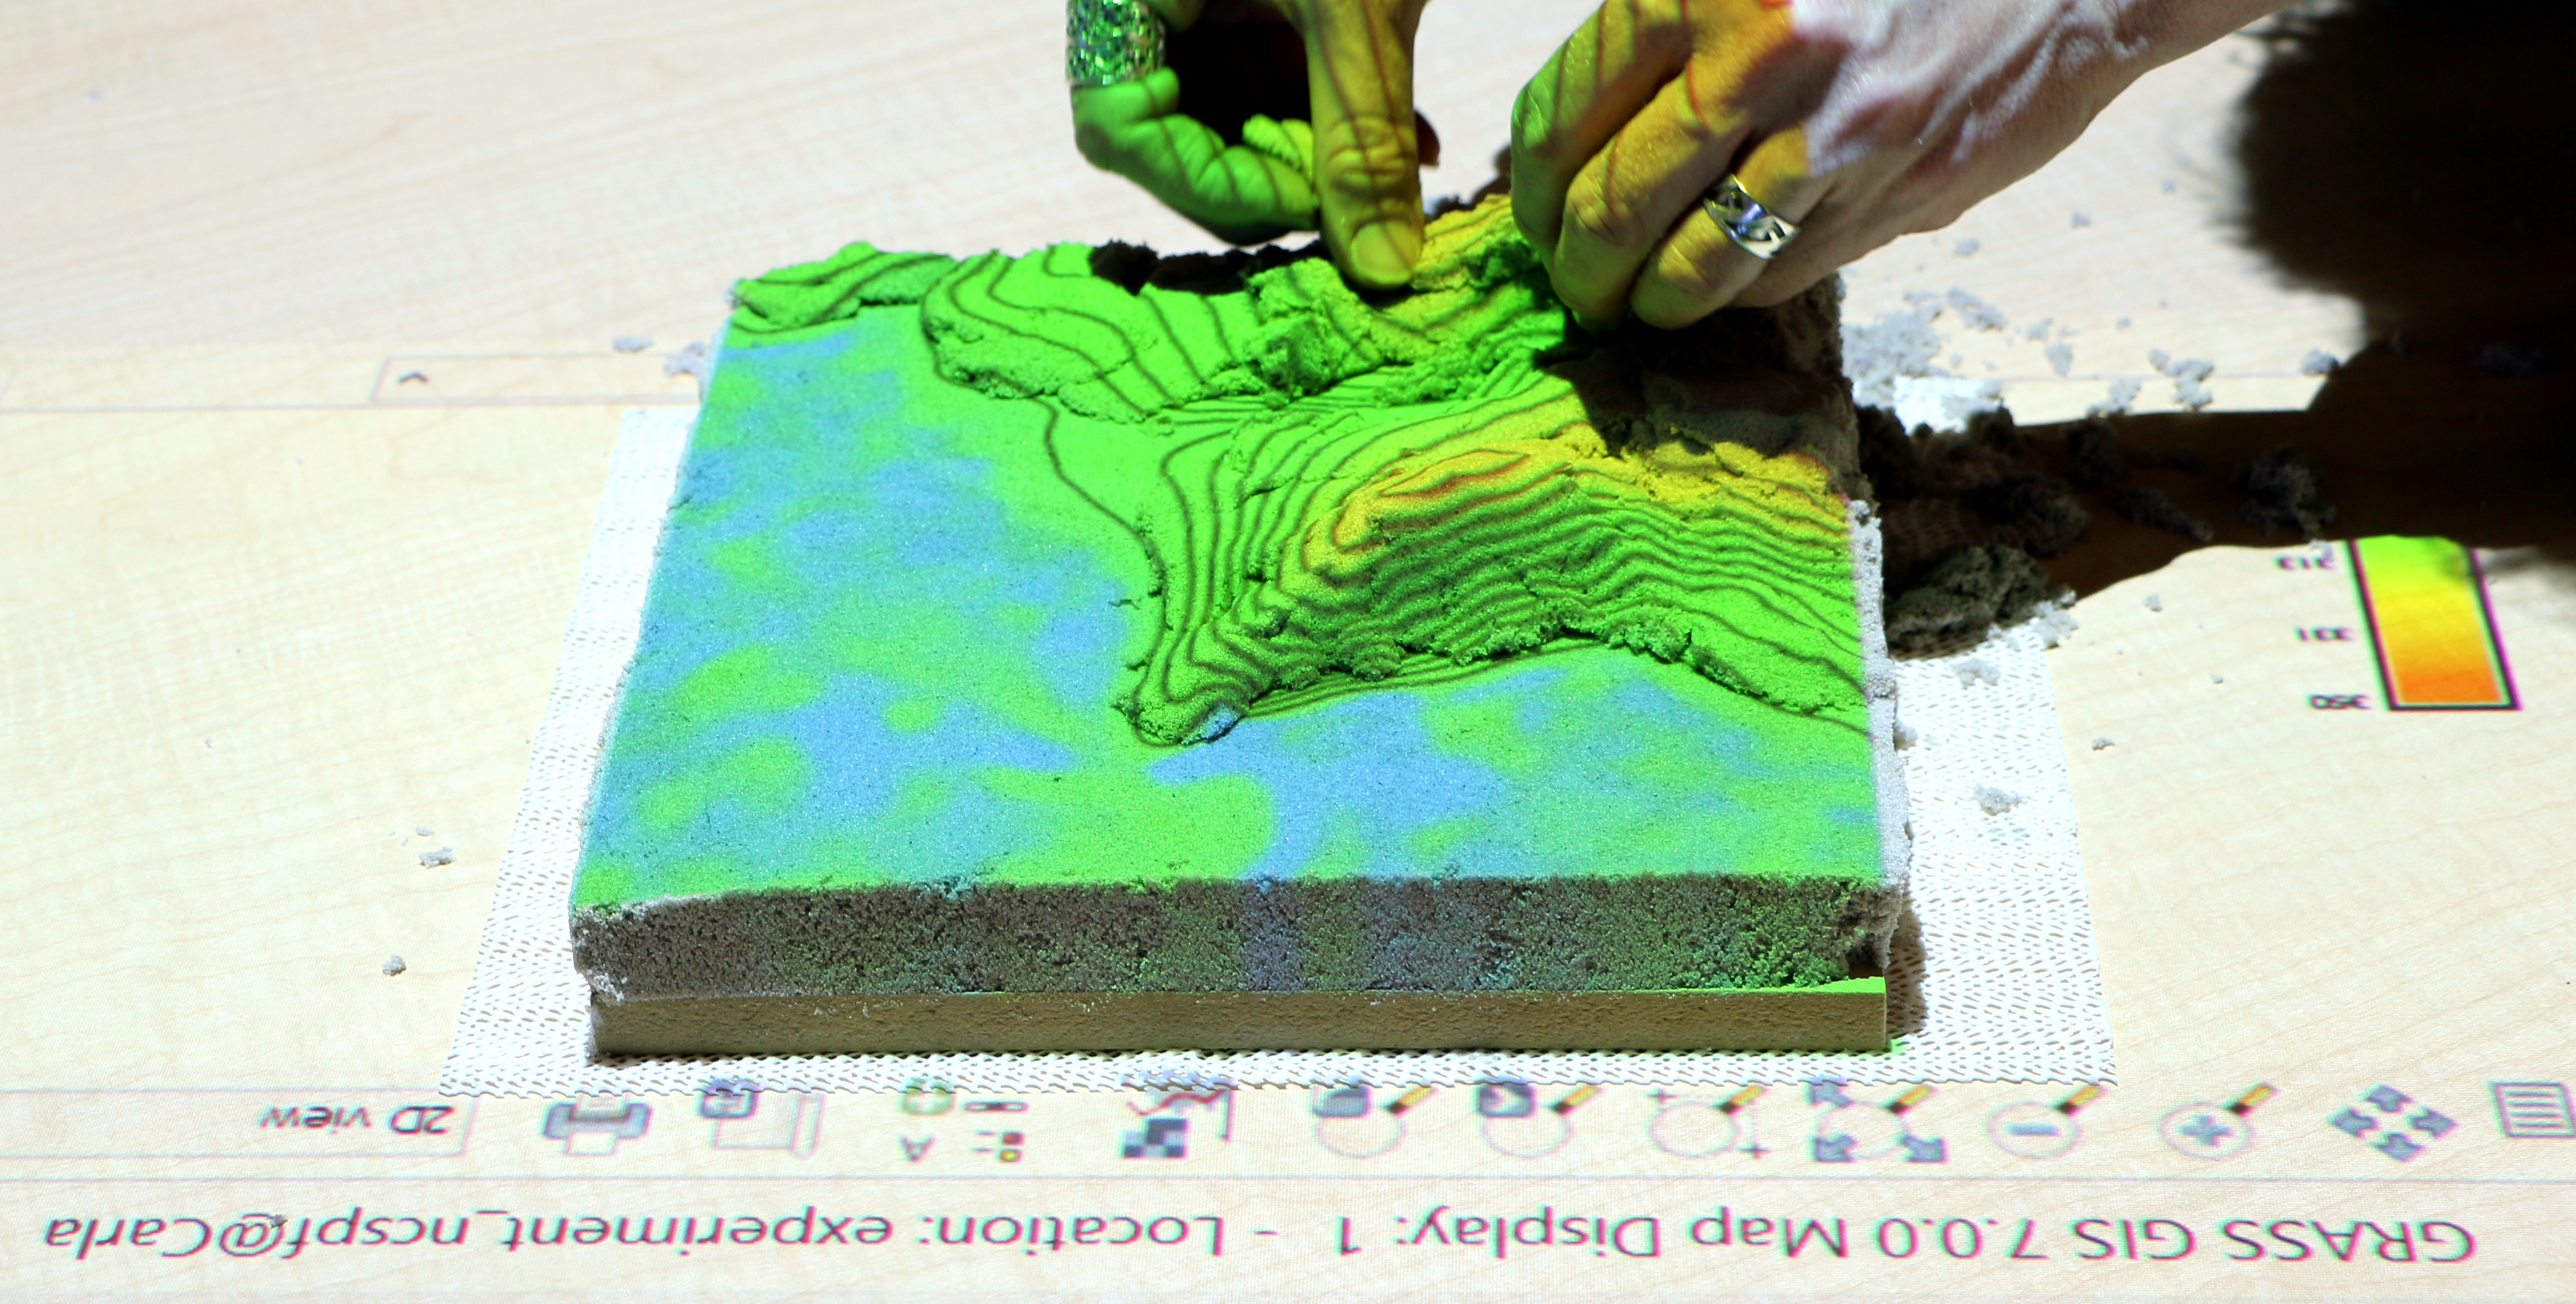
\includegraphics[width=\textwidth]{images/experiments/carla_proj_aug.jpg}
	\caption{Coupling experiment - projection-augmented modeling:
	A participant sculpts the study landscape using
	the projected elevation and contour maps
	as guides.}
	\label{fig:proj_aug}
\end{center}
\end{figure}


\paragraph{Digital modeling}
Participants had 10 minutes to digitally model the study landscape in Rhinoceros 5, 
a non-uniform rational basis spline (NURBS) based 3D modeling program
designed for precise freeform curve and surface modeling \cite{Rhino}.
After 10 minutes of training 
participants modeled the study landscape as a NURBS surface 
by vertically translating control points (Fig.~\ref{fig:rhino}). 
They started with a flat NURBS surface that was 
divided into a 10 x 10 grid of control points.
As a reference their model space also included 
a locked 3D representation of the study landscape as contours. 
At any point participants could rebuild the surface 
with a higher density of control points for finer, more nuanced control. 
This method is relatively simple and 
analogous to basic actions in sculpture -- pushing and pulling. 
We developed and tested this method 
as a simple, straightforward digital freeform surface modeling technique
that could be taught quickly, yet could produce an accurate model. 
%  
% timing / rebuilding
Through testing we determined that 
novice users took approximately 10 minutes
to model the surface with a 10 x 10 grid of control points
before wanting to building the surface with more control points.
%
See Appendix \ref{appendix:videos}
for videos demonstrating the training \ref{videos:training} and digital 3D modeling task (\ref{videos:digital}).

% choice of 3d modeling program
Different 3D modeling programs afford very different
interactions, modeling tools, data structures, and modes of representations. 
%
Developing a simple, intuitive modeling technique 
drove the choice of software in this study. 
%
After testing 3D modeling workflows in 
Rhinoceros, Vue, Maya, SketchUp, and Voxel Builder
we chose Rhinoceros for this task because it 
is popular with designers such as architects, 
has a wide variety of modeling tools,
can precisely represent continuous surfaces, 
and has plugins for importing and exporting geographic data. 
%
To make a fair comparison between digital, analog, and tangible modeling,
the digital modeling technique needed to be relatively analogous to hand sculpting
-- i.e.~pushing and pulling rather than painting in 3D, drafting in 3D, or stacking voxels.
%
There is an analogous modeling technique -- pulling and pushing vertices -- 
using the Sandbox tool in SketchUp \cite{SketchUp},
but this creates a triangulated irregular network (TIN)
rather than a continuous NURBS surface. 
%
Vue has a terrain editor designed for intuitive 3D painting and sculpting \cite{Vue},
but it requires continual retuning of tool parameters
and generates a TIN. 
%
TINs less accurately represent continuous surfaces like topography
and would generate artifacts in our analyses. 
%
In another pilot study \cite{Harmon2016} we tested Vue's terrain editor. 
We found that participants tended to 
over-exaggerate distinct features in the landscape like stream channels, 
while ignoring more subtle features like slopes.  
We also determined that the resulting models
had an obvious triangulated structure that caused
exaggerated slopes and discontinuous water flow 
in our analyses. 
%
While voxel modeling programs 
%like Voxel Builder % http://voxelbuilder.com/
%and MagicaVoxel % https://ephtracy.github.io/
and games like Minecraft \cite{Minecraft}
are very intuitive to use,
they can also be slow to use,
create blocky rather than
continuous surfaces, 
and are not typically used in design professions 
like architecture and landscape architecture.

\paragraph{Analog modeling}

After a brief explanation and demonstration
participants had 10 minutes to sculpt the study landscape in polymer-enriched sand 
by hand or with a wooden sculpting tool (Fig.~\ref{fig:analog}).  
They were given a CNC-routed model of the study landscape 
as a reference, a sculpting tool, and a 3D scale. 
Participants were shown how the 3D scale could be used to 
measure the height of the model. 
A lamp on the table cast shadows across the model for hillshading.
%
See Appendix \ref{appendix:videos}
for a video demonstrating the analog 3D modeling task (\ref{videos:analog}).

\paragraph{Projection-augmented modeling}
After a minute long explanation and demonstration
participants had 10 minutes to sculpt
a projection-augmented, polymer-enriched sand model
of the study landscape by hand or with a wooden sculpting tool 
(Fig.~\ref{fig:proj_aug}). 
Tangible Landscape was used to project 
an elevation map of the study landscape
with contours and a legend
onto participants' sand models as guide for sculpting. 
Participants were also given CNC routed reference model and 
a 3D scale ruled in map units. 
After an explanation of the contour map, elevation color table, and legend,
participants were shown how the 3D scale could be used to 
measure the elevation of their scale models
%
See Appendix \ref{appendix:videos}
for a video demonstrating the projection-augmented 3D modeling task (\ref{videos:augmented}).

\paragraph{Data collection and analysis}
We used Tangible Landscape to scan the finished models 
built using analog hand modeling and projection-augmented modeling.
The scans were captured as point clouds, interpolated 
as digital elevation models using the regularized spline with tension method,
and stored as raster maps in a GRASS GIS database 
The NURBS surfaces modeled in Rhinoceros were exported as raster elevation maps,
imported into GRASS GIS, randomly resampled, 
re-interpolated using the regularized spline with tension method, 
and stored as raster maps in a GRASS GIS database. 
The data from Rhinoceros was randomly resampled and re-interpolated
to account for differences and irregularities in resolution, data density, and point spacing.

For each set of models -- digital, analog, and augmented --
we computed cellular statistics (i.e.~per cell statistics), 
topographic and morphometric parameters, 
and simulated water flow.

\paragraph{Mean elevation}
We computed 
the mean elevation 
and standard deviation of elevation
for each set
with the module \textit{r.series} \cite{r.series}.
The mean elevation is the average of each cell 
of all elevation maps in a given set of models.

\paragraph{Standard deviation of elevation}
We computed 
the standard deviation of elevation
for each set
with the module \textit{r.series} \cite{r.series}.
This is the standard deviation of each cell 
of all elevation maps in a given set of models.
We used a sequential color table from Color Brewer
\cite{Brewer1994,ColorBrewer}.

\paragraph{Mean difference}
In order to compare participants' modeling performance between sets 
we computed the difference 
between the linearly regressed reference elevation and 
the mean elevation for each set.
%
The difference between the reference and mean elevation maps should show
where the mean elevation values for each set are too low or too high. 
%
There were, however, systematic errors in the scanned models.
%
Table \ref{table:scatterplots} shows the vertical shift 
in the hand sculpted and projection-augmented models 
caused by scanning and georeferencing.
%
We used linear regression 
%the linear regression of the reference and mean elevation maps
%calculated with the module \textit{r.regression.line} \cite{r.regression.line}
to vertically rescale and translate the reference elevation 
in order to account for these systematic errors
in the difference calculation,

\begin{equation}
\label{eq:regressed_mean_difference}
\Delta = (a + b * z_0) - \overline{z}
\end{equation}

where:

\hspace*{1em} $\Delta$ is the difference

\hspace*{1em} $z_0$ is the reference elevation map

\hspace*{1em} $\overline{z}$ is the mean elevation of maps in a set

\hspace*{1em} $a$ is the intercept of the regression line

\hspace*{1em} $b$ is the slope of the regression line.\\


\paragraph{Standard deviation of difference}

We computed the standard deviation of difference
by first calculating the difference 
between the linearly regressed reference elevation and 
each modeled elevation map in a set
to generate a set of difference maps.
Then we calculated the standard deviation 
for that set of difference maps. 

%\begin{equation}
%\label{eq:regressed_difference}
%\sigma(\Delta) = (a + b * z_0) - z % add stdev to this side of the equation
%\end{equation}
%
%where:
%
%\hspace*{1em} $\sigma$ is the standard deviation
%
%\hspace*{1em} $\Delta$ is the difference
%
%\hspace*{1em} $z_0$ is the reference elevation map
%
%\hspace*{1em} $z$ is a modeled elevation map
%
%\hspace*{1em} $a$ is the intercept of the regression line
%
%\hspace*{1em} $b$ is the slope of the regression line.\\

\paragraph{Mean slope}
We derived the slope of the mean elevation of each set %in degrees
using differential geometry
%by parameterizing a quadratic function to fit mean elevation values 
%in a neighborhood using least squares 
\cite{Wood1996} 
%through quadratic parameterization \cite{Wood1996} of the mean digital elevation model 
with the module \textit{r.param.scale} \cite{r.param.scale}.

\paragraph{Mean landforms}
We identified landforms 
for the mean digital elevation model for each set 
using geomorphon,
a pattern recognition method for landform classification 
based on the openness of the terrain
implemented as the add-on module \textit{r.geomorphon} \cite{r.geomorphon}.
Geomorphon works effectively across spatial scales because 
the neighborhood search size for pattern recognition 
is spatially variable -- it depends on the visibility of the cell \cite{Jasiewicz2013}.  
Landforms can be classified as flat, peak, ridge, shoulder, spur, slope, hollow, footslope, valley, or depression (Fig.~\ref{fig:geomorphons}).

\paragraph{Mean minimum distance}
We also computed the mean minimum distance between features 
such as concentrated water flow, ridges, and valleys
on the modeled landscapes and the reference landscape.

\paragraph{Systematic errors}
Table \ref{table:scatterplots} shows systematic errors
in the hand sculpted and projection-augmented models.
These models are vertically shifted due to scanning
and have low values along the borders
caused by slumping sand. 
While we used linear regression 
to vertically shift and rescale the difference in elevation, 
we did not mitigate the systematic errors
along the borders. 


\begin{table}
\tbl{Bivariate scatterplots of elevation values}{
\ra{1.3}
\begin{tabular}{m{0.05\textwidth} m{0.3\textwidth} m{0.3\textwidth} m{0.3\textwidth}}
\toprule
& \multicolumn{1}{c}{Digital} & \multicolumn{1}{c}{Analog}  & \multicolumn{1}{c}{Augmented}\\
\midrule \\
Mean & 
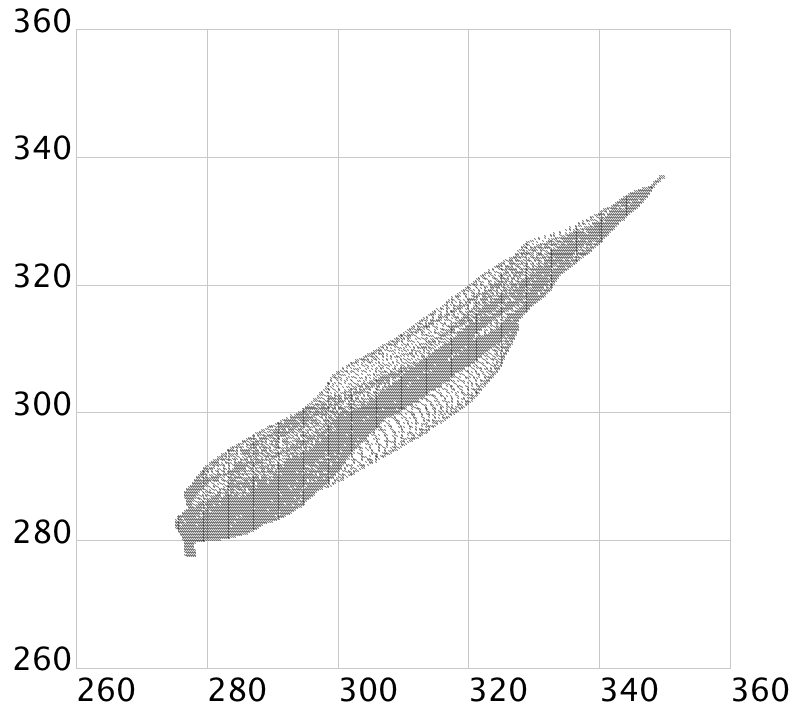
\includegraphics[width=0.3\textwidth]{images/bivariate_scatterplots/dem_1.png} &
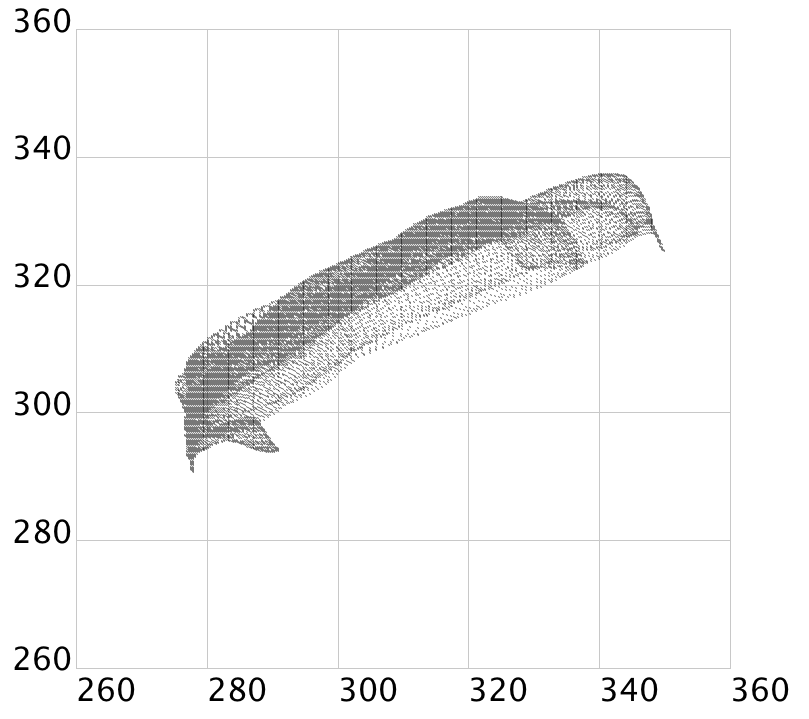
\includegraphics[width=0.3\textwidth]{images/bivariate_scatterplots/dem_2.png} &
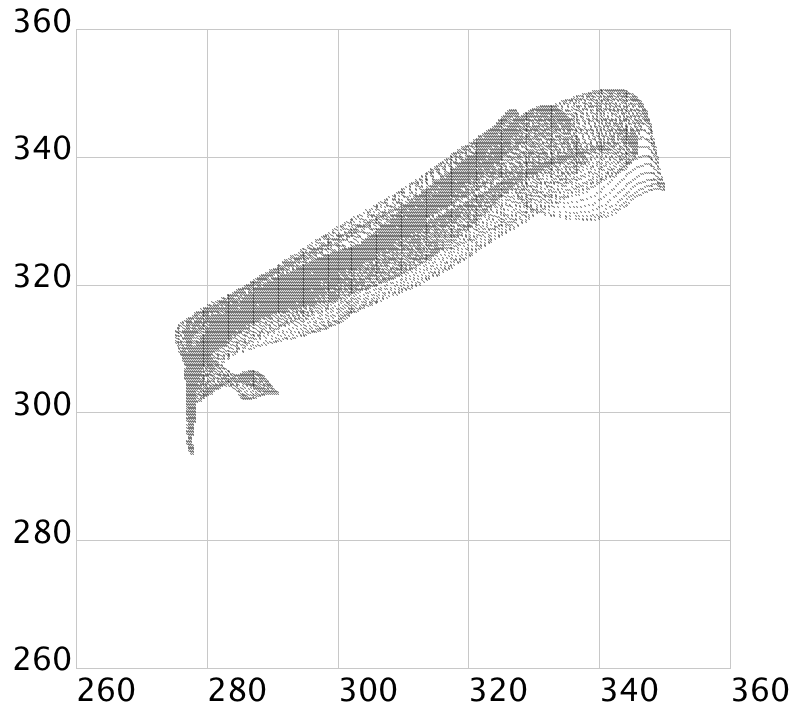
\includegraphics[width=0.3\textwidth]{images/bivariate_scatterplots/dem_3.png}\\
& \multicolumn{1}{c}{Reference} & \multicolumn{1}{c}{Reference} & \multicolumn{1}{c}{Reference} \\
\\
\bottomrule
\end{tabular}}
\label{table:scatterplots} 
\end{table}

% landform legend
\begin{figure}
\begin{center}
		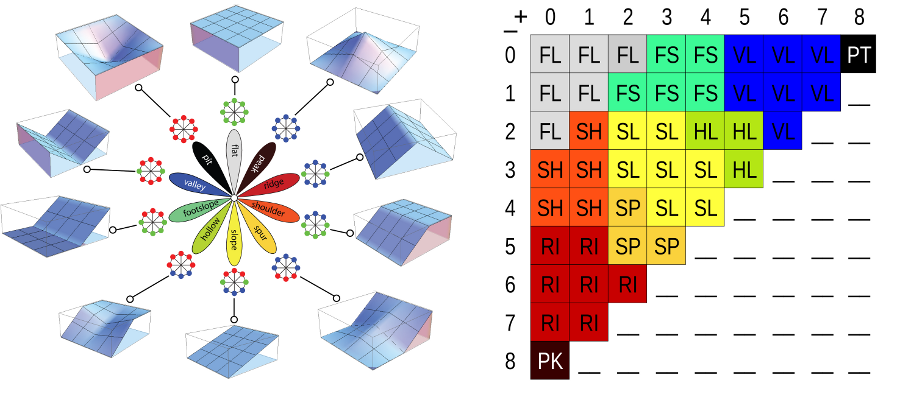
\includegraphics[width=\textwidth]{images/geomorphons_legend.png}
	\caption{Landforms identified by \textit{r.geomorphon} --
		1)~flat, 
		2)~peak, 
		3)~ridge, 
		4)~shoulder, 
		5)~spur, 
		6)~slope, 
		7)~hollow, 
		8)~footslope, 
		9)~valley, and
		10)~depression.
		Source: \cite{r.geomorphon}.}
	\label{fig:geomorphons}
\end{center}
\end{figure}

% ---------------------------- REVISIONS ---------------------------- 
% 
% Revised color table
% 	Add reference to Brewer & Brewer / Color Brewer
%
% -------------------------------------------------------------------------- 

% REFEREE 2:
%- This is just personal preference, but I found the Figures of results in the previous 2016 TEI paper by Harmon, which show a 2D top-down view, more readable than the smaller 3D renderings in this article. But this is not a criticism, just personal preference. I was also interested in the choice of color scheme for the heat maps, some of which I also found harder to read than others. An example are the colors for the stdev. of difference in Table VI. The authors may have a good reason for these colors - the choice for mean difference colors for user feedback seems for instance very clear. Some may also be standard in the GIS community, in which case it would be helpful to include a reference.

\subsection{Results}
%
%Participants digitally modeled so approximately and abstractly 
%with Rhinoceros
%that they only hinted at landforms. % at the morphology.
%%
%When they sculpted by hand
%their models tended to be descriptive -- 
%differing substantially from the reference, but
%accurately representing most of the landforms. 
%%
%Their performance improved 
%when they sculpted projection-augmented models --
%the resulting models
%fit the reference better, 
%had more defined topography, 
%and accurately represented most of the landforms.
%%
%Table \ref{table:scatterplots} shows systematic errors
%in the hand sculpted and projection-augmented models;
%these models are vertically shifted due to scanning
%and have low values along the borders
%caused by slumping sand. 
%While we used linear regression 
%to vertically shift and rescale the difference in elevation, 
%we did not mitigate the systematic errors
%along the borders. 
%%
%Table \ref{table:coupling_experiment} shows 3D maps of cellular statistics 
%and geospatial analyses for this experiment.

% ---------------------------- TREE ---------------------------- 

\begin{figure}
\begin{center}
%
\begin{tikzpicture}[grow = right,
	level 1/.style={sibling distance=12 em},
	level 2/.style={sibling distance=6 em},
	level distance = 14em,
	every node/.style = {shape=rectangle, 
		rounded corners,
		draw, 
		font=\footnotesize,
		align=center,
		top color=white,
		bottom color=white}]
\node {Participants \\ 
	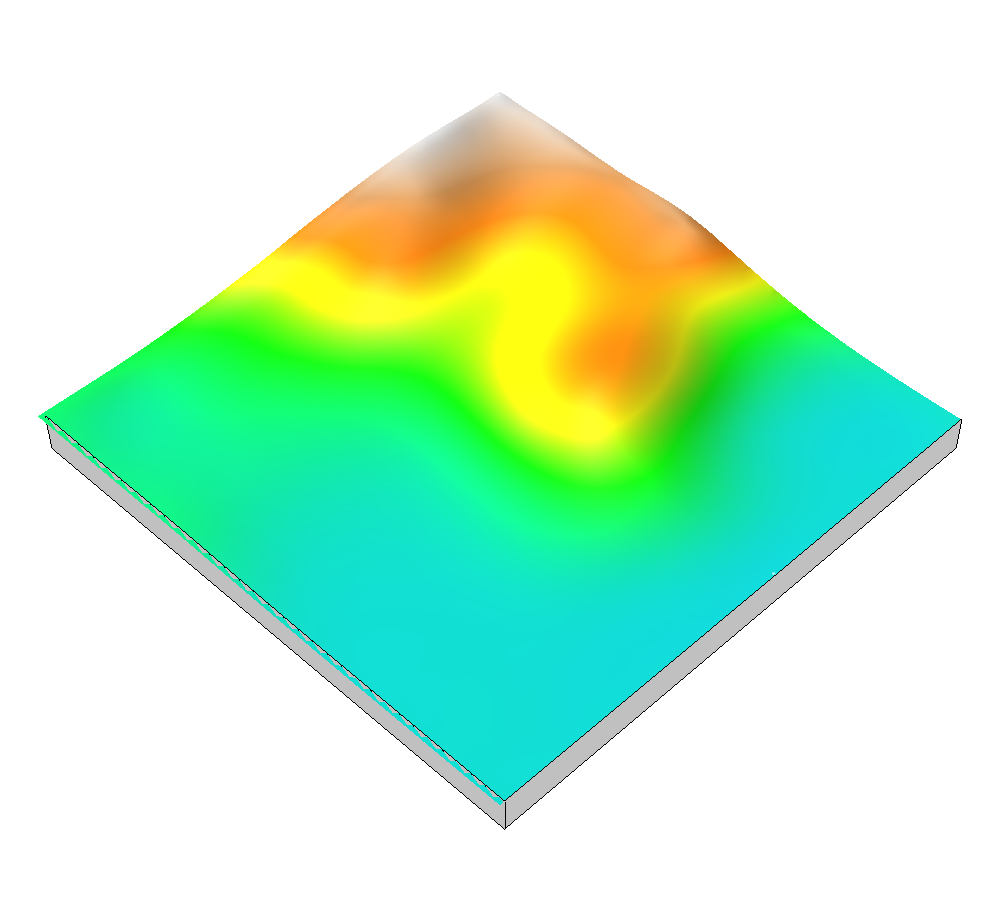
\includegraphics[width=0.1\textwidth]{images/render_3d/participants/mean_dem_1.png}
	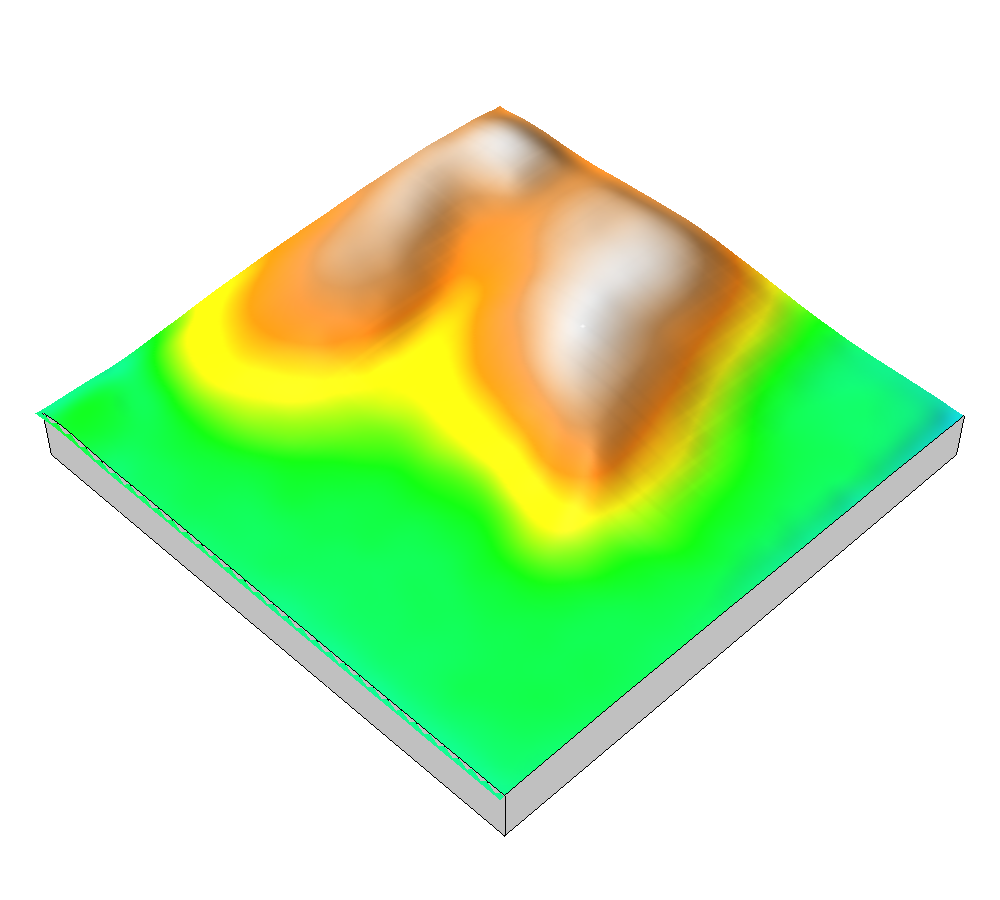
\includegraphics[width=0.1\textwidth]{images/render_3d/participants/mean_dem_2.png}
	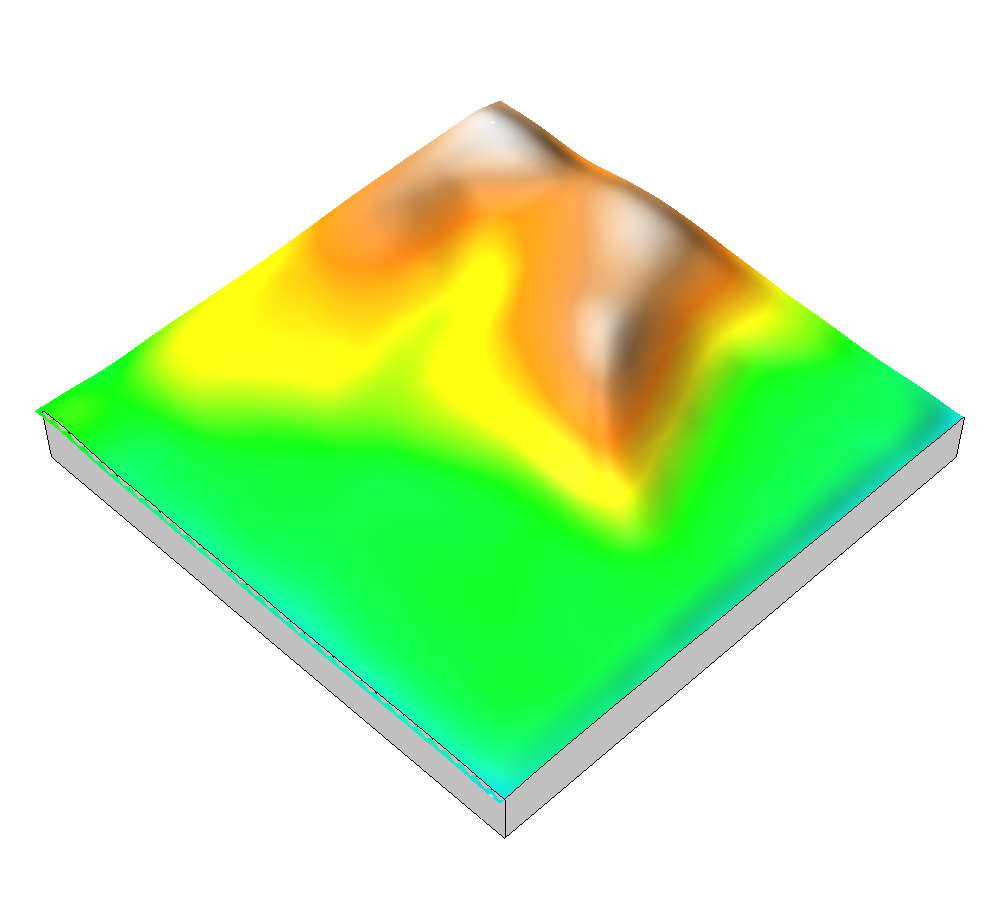
\includegraphics[width=0.1\textwidth]{images/render_3d/participants/mean_dem_3.png} \\
	\makebox[0.1\textwidth][c]{\scriptsize Digital}
	\makebox[0.1\textwidth][c]{\scriptsize Analog }
	\makebox[0.1\textwidth][c]{\scriptsize Augmented }
	}
	child { node {Students \\ 
		\includegraphics[width=0.1\textwidth]{images/render_3d/students/mean_dem_1.png}
		\includegraphics[width=0.1\textwidth]{images/render_3d/students/mean_dem_2.png}
		\includegraphics[width=0.1\textwidth]{images/render_3d/students/mean_dem_3.png}
		}
		child { node {Landscape architecture \\ 
			\includegraphics[width=0.1\textwidth]{images/render_3d/landscape_students/mean_dem_1.png}
			\includegraphics[width=0.1\textwidth]{images/render_3d/landscape_students/mean_dem_2.png}
			\includegraphics[width=0.1\textwidth]{images/render_3d/landscape_students/mean_dem_3.png}
			}
			}
		child { node {GIS \\ 
			\includegraphics[width=0.1\textwidth]{images/render_3d/gis_students/mean_dem_1.png}
			\includegraphics[width=0.1\textwidth]{images/render_3d/gis_students/mean_dem_2.png}
			\includegraphics[width=0.1\textwidth]{images/render_3d/gis_students/mean_dem_3.png}
			}
			}
		}
	child { node {Professionals \\ 
		\includegraphics[width=0.1\textwidth]{images/render_3d/professionals/mean_dem_1.png}
		\includegraphics[width=0.1\textwidth]{images/render_3d/professionals/mean_dem_2.png}
		\includegraphics[width=0.1\textwidth]{images/render_3d/professionals/mean_dem_3.png}
		}
		child { node {3D novices \\ 
			\includegraphics[width=0.1\textwidth]{images/render_3d/3d_novices/mean_dem_1.png}
			\includegraphics[width=0.1\textwidth]{images/render_3d/3d_novices/mean_dem_2.png}
			\includegraphics[width=0.1\textwidth]{images/render_3d/3d_novices/mean_dem_3.png}
			}
			}
		child { node {3D experts \\ 
			\includegraphics[width=0.1\textwidth]{images/render_3d/3d_experts/mean_dem_1.png}
			\includegraphics[width=0.1\textwidth]{images/render_3d/3d_experts/mean_dem_2.png}
			\includegraphics[width=0.1\textwidth]{images/render_3d/3d_experts/mean_dem_3.png}
			}
			}
};
\end{tikzpicture}
%
\caption{Pairwise comparison of the mean digital elevation models grouped by category of participants}
\label{fig:tree}
\end{center}
\end{figure}

% ---------------------------- PARTICIPANTS ---------------------------- 

\begin{table}
\tbl{Coupling experiment: maps of per-cell statistics and geospatial analyses draped over 3D topography for all participants}{
\ra{1.3}
\begin{tabular}{m{0.19\textwidth} m{0.19\textwidth} m{0.19\textwidth} m{0.19\textwidth} m{0.19\textwidth}}
\toprule
& \multicolumn{1}{c}{Reference} & \multicolumn{1}{c}{Digital} & \multicolumn{1}{c}{Analog}  & \multicolumn{1}{c}{Augmented}\\
\midrule
%
Mean elevation \par \vspace{0.5em} \includegraphics[width=0.19\textwidth]{images/legends/elevation_legend_1.pdf} & 
\includegraphics[width=0.19\textwidth]{images/render_3d/participants/dem_1.png} &
\includegraphics[width=0.19\textwidth]{images/render_3d/participants/mean_dem_1.png} &
\includegraphics[width=0.19\textwidth]{images/render_3d/participants/mean_dem_2.png} &
\includegraphics[width=0.19\textwidth]{images/render_3d/participants/mean_dem_3.png}\\
%
Stdev.~of elevations \par \vspace{0.5em} \includegraphics[width=0.19\textwidth]{images/legends/stdev_legend.pdf} & 
\includegraphics[width=0.19\textwidth]{images/render_3d/participants/dem_difference_1.png} &
\includegraphics[width=0.19\textwidth]{images/render_3d/participants/stdev_dem_1.png} &
\includegraphics[width=0.19\textwidth]{images/render_3d/participants/stdev_dem_2.png} &
\includegraphics[width=0.19\textwidth]{images/render_3d/participants/stdev_dem_3.png}\\
%
Stdev.~of difference \par \vspace{0.5em} \includegraphics[width=0.19\textwidth]{images/legends/stdev_diff_legend.pdf} & 
\includegraphics[width=0.19\textwidth]{images/render_3d/participants/dem_difference_1.png} &
\includegraphics[width=0.19\textwidth]{images/render_3d/participants/stdev_regression_difference_series_1.png} &
\includegraphics[width=0.19\textwidth]{images/render_3d/participants/stdev_regression_difference_series_2.png} &
\includegraphics[width=0.19\textwidth]{images/render_3d/participants/stdev_regression_difference_series_3.png}\\
%
Mean difference \par \vspace{0.5em} \includegraphics[width=0.19\textwidth]{images/legends/diff_legend.pdf} & 
\includegraphics[width=0.19\textwidth]{images/render_3d/participants/dem_difference_1.png} &
\includegraphics[width=0.19\textwidth]{images/render_3d/participants/mean_dem_regression_difference_1.png} &
\includegraphics[width=0.19\textwidth]{images/render_3d/participants/mean_dem_regression_difference_2.png} &
\includegraphics[width=0.19\textwidth]{images/render_3d/participants/mean_dem_regression_difference_3.png}\\
%
Mean slope \par \vspace{0.5em} \includegraphics[width=0.19\textwidth]{images/legends/slope_legend.pdf} & 
\includegraphics[width=0.19\textwidth]{images/render_3d/participants/slope_1.png} &
\includegraphics[width=0.19\textwidth]{images/render_3d/participants/mean_slope_1.png} &
\includegraphics[width=0.19\textwidth]{images/render_3d/participants/mean_slope_2.png} &
\includegraphics[width=0.19\textwidth]{images/render_3d/participants/mean_slope_3.png}\\
%
Mean landforms \par \vspace{0.5em} \includegraphics[width=0.19\textwidth]{images/legends/forms_legend.pdf} & 
\includegraphics[width=0.19\textwidth]{images/render_3d/participants/forms_1.png} &
\includegraphics[width=0.19\textwidth]{images/render_3d/participants/mean_forms_1.png} &
\includegraphics[width=0.19\textwidth]{images/render_3d/participants/mean_forms_2.png} &
\includegraphics[width=0.19\textwidth]{images/render_3d/participants/mean_forms_3.png}\\
%
\bottomrule
\end{tabular}}
\label{table:coupling_experiment} 
\end{table}

% ---------------------------- STUDENTS vs PROFESSIONALS ---------------------------- 

% STUDENTS

\begin{table}
\tbl{Students}{
\ra{1.3}
\begin{tabular}{m{0.19\textwidth} m{0.19\textwidth} m{0.19\textwidth} m{0.19\textwidth} m{0.19\textwidth}}
\toprule
& \multicolumn{1}{c}{Reference} & \multicolumn{1}{c}{Digital} & \multicolumn{1}{c}{Analog}  & \multicolumn{1}{c}{Augmented}\\
\midrule
%
Mean elevation \par \vspace{0.5em} \includegraphics[width=0.19\textwidth]{images/legends/elevation_legend_1.pdf} & 
\includegraphics[width=0.19\textwidth]{images/render_3d/students/dem_1.png} &
\includegraphics[width=0.19\textwidth]{images/render_3d/students/mean_dem_1.png} &
\includegraphics[width=0.19\textwidth]{images/render_3d/students/mean_dem_2.png} &
\includegraphics[width=0.19\textwidth]{images/render_3d/students/mean_dem_3.png}\\
%
Stdev.~of difference \par \vspace{0.5em} \includegraphics[width=0.19\textwidth]{images/legends/stdev_diff_legend.pdf} & 
\includegraphics[width=0.19\textwidth]{images/render_3d/students/dem_difference_1.png} &
\includegraphics[width=0.19\textwidth]{images/render_3d/students/stdev_regression_difference_series_1.png} &
\includegraphics[width=0.19\textwidth]{images/render_3d/students/stdev_regression_difference_series_2.png} &
\includegraphics[width=0.19\textwidth]{images/render_3d/students/stdev_regression_difference_series_3.png}\\
%
Mean landforms \par \vspace{0.5em} \includegraphics[width=0.19\textwidth]{images/legends/forms_legend.pdf} & 
\includegraphics[width=0.19\textwidth]{images/render_3d/students/forms_1.png} &
\includegraphics[width=0.19\textwidth]{images/render_3d/students/mean_forms_1.png} &
\includegraphics[width=0.19\textwidth]{images/render_3d/students/mean_forms_2.png} &
\includegraphics[width=0.19\textwidth]{images/render_3d/students/mean_forms_3.png}\\
%
\bottomrule
\end{tabular}}
\label{table:students} 

% PROFESSIONALS
\vspace*{1.5em}

\tbl{Academics and professionals}{
\ra{1.3}
\begin{tabular}{m{0.19\textwidth} m{0.19\textwidth} m{0.19\textwidth} m{0.19\textwidth} m{0.19\textwidth}}
\toprule
& \multicolumn{1}{c}{Reference} & \multicolumn{1}{c}{Digital} & \multicolumn{1}{c}{Analog}  & \multicolumn{1}{c}{Augmented}\\
\midrule
%
Mean elevation \par \vspace{0.5em} \includegraphics[width=0.19\textwidth]{images/legends/elevation_legend_1.pdf} & 
\includegraphics[width=0.19\textwidth]{images/render_3d/professionals/dem_1.png} &
\includegraphics[width=0.19\textwidth]{images/render_3d/professionals/mean_dem_1.png} &
\includegraphics[width=0.19\textwidth]{images/render_3d/professionals/mean_dem_2.png} &
\includegraphics[width=0.19\textwidth]{images/render_3d/professionals/mean_dem_3.png}\\
%
Stdev.~of difference \par \vspace{0.5em} \includegraphics[width=0.19\textwidth]{images/legends/stdev_diff_legend.pdf} & 
\includegraphics[width=0.19\textwidth]{images/render_3d/professionals/dem_difference_1.png} &
\includegraphics[width=0.19\textwidth]{images/render_3d/professionals/stdev_regression_difference_series_1.png} &
\includegraphics[width=0.19\textwidth]{images/render_3d/professionals/stdev_regression_difference_series_2.png} &
\includegraphics[width=0.19\textwidth]{images/render_3d/professionals/stdev_regression_difference_series_3.png}\\
%
Mean landforms \par \vspace{0.5em} \includegraphics[width=0.19\textwidth]{images/legends/forms_legend.pdf} & 
\includegraphics[width=0.19\textwidth]{images/render_3d/professionals/forms_1.png} &
\includegraphics[width=0.19\textwidth]{images/render_3d/professionals/mean_forms_1.png} &
\includegraphics[width=0.19\textwidth]{images/render_3d/professionals/mean_forms_2.png} &
\includegraphics[width=0.19\textwidth]{images/render_3d/professionals/mean_forms_3.png}\\
%
\bottomrule
\end{tabular}}
\label{table:professionals} 
\end{table}

% ---------------------------- LANDSCAPE vs. GIS STUDENTS ---------------------------- 

% LANDSCAPE STUDENTS

\begin{table}
\tbl{Landscape architecture students}{
\ra{1.3}
\begin{tabular}{m{0.19\textwidth} m{0.19\textwidth} m{0.19\textwidth} m{0.19\textwidth} m{0.19\textwidth}}
\toprule
& \multicolumn{1}{c}{Reference} & \multicolumn{1}{c}{Digital} & \multicolumn{1}{c}{Analog}  & \multicolumn{1}{c}{Augmented}\\
\midrule
%
Mean elevation \par \vspace{0.5em} \includegraphics[width=0.19\textwidth]{images/legends/elevation_legend_1.pdf} & 
\includegraphics[width=0.19\textwidth]{images/render_3d/landscape_students/dem_1.png} &
\includegraphics[width=0.19\textwidth]{images/render_3d/landscape_students/mean_dem_1.png} &
\includegraphics[width=0.19\textwidth]{images/render_3d/landscape_students/mean_dem_2.png} &
\includegraphics[width=0.19\textwidth]{images/render_3d/landscape_students/mean_dem_3.png}\\
%
Stdev.~of difference \par \vspace{0.5em} \includegraphics[width=0.19\textwidth]{images/legends/stdev_diff_legend.pdf} & 
\includegraphics[width=0.19\textwidth]{images/render_3d/landscape_students/dem_difference_1.png} &
\includegraphics[width=0.19\textwidth]{images/render_3d/landscape_students/stdev_regression_difference_series_1.png} &
\includegraphics[width=0.19\textwidth]{images/render_3d/landscape_students/stdev_regression_difference_series_2.png} &
\includegraphics[width=0.19\textwidth]{images/render_3d/landscape_students/stdev_regression_difference_series_3.png}\\
%
Mean landforms \par \vspace{0.5em} \includegraphics[width=0.19\textwidth]{images/legends/forms_legend.pdf} & 
\includegraphics[width=0.19\textwidth]{images/render_3d/landscape_students/forms_1.png} &
\includegraphics[width=0.19\textwidth]{images/render_3d/landscape_students/mean_forms_1.png} &
\includegraphics[width=0.19\textwidth]{images/render_3d/landscape_students/mean_forms_2.png} &
\includegraphics[width=0.19\textwidth]{images/render_3d/landscape_students/mean_forms_3.png}\\
%
\bottomrule
\end{tabular}}
\label{table:landscape_students} 

% GIS STUDENTS
\vspace*{1.5em}

\tbl{GIS students}{
\ra{1.3}
\begin{tabular}{m{0.19\textwidth} m{0.19\textwidth} m{0.19\textwidth} m{0.19\textwidth} m{0.19\textwidth}}
\toprule
& \multicolumn{1}{c}{Reference} & \multicolumn{1}{c}{Digital} & \multicolumn{1}{c}{Analog}  & \multicolumn{1}{c}{Augmented}\\
\midrule
%
Mean elevation \par \vspace{0.5em} \includegraphics[width=0.19\textwidth]{images/legends/elevation_legend_1.pdf} & 
\includegraphics[width=0.19\textwidth]{images/render_3d/gis_students/dem_1.png} &
\includegraphics[width=0.19\textwidth]{images/render_3d/gis_students/mean_dem_1.png} &
\includegraphics[width=0.19\textwidth]{images/render_3d/gis_students/mean_dem_2.png} &
\includegraphics[width=0.19\textwidth]{images/render_3d/gis_students/mean_dem_3.png}\\
%
Stdev.~of difference \par \vspace{0.5em} \includegraphics[width=0.19\textwidth]{images/legends/stdev_diff_legend.pdf} & 
\includegraphics[width=0.19\textwidth]{images/render_3d/gis_students/dem_difference_1.png} &
\includegraphics[width=0.19\textwidth]{images/render_3d/gis_students/stdev_regression_difference_series_1.png} &
\includegraphics[width=0.19\textwidth]{images/render_3d/gis_students/stdev_regression_difference_series_2.png} &
\includegraphics[width=0.19\textwidth]{images/render_3d/gis_students/stdev_regression_difference_series_3.png}\\
%
Mean landforms \par \vspace{0.5em} \includegraphics[width=0.19\textwidth]{images/legends/forms_legend.pdf} & 
\includegraphics[width=0.19\textwidth]{images/render_3d/gis_students/forms_1.png} &
\includegraphics[width=0.19\textwidth]{images/render_3d/gis_students/mean_forms_1.png} &
\includegraphics[width=0.19\textwidth]{images/render_3d/gis_students/mean_forms_2.png} &
\includegraphics[width=0.19\textwidth]{images/render_3d/gis_students/mean_forms_3.png}\\
%
\bottomrule
\end{tabular}}
\label{table:gis_students} 
\end{table}

% ---------------------------- 3D NOVICES vs EXPERTS ---------------------------- 

% 3D NOVICES

\begin{table}
\tbl{Academics and professionals without expertise in 3D modeling}{
\ra{1.3}
\begin{tabular}{m{0.19\textwidth} m{0.19\textwidth} m{0.19\textwidth} m{0.19\textwidth} m{0.19\textwidth}}
\toprule
& \multicolumn{1}{c}{Reference} & \multicolumn{1}{c}{Digital} & \multicolumn{1}{c}{Analog}  & \multicolumn{1}{c}{Augmented}\\
\midrule
%
Mean elevation \par \vspace{0.5em} \includegraphics[width=0.19\textwidth]{images/legends/elevation_legend_1.pdf} & 
\includegraphics[width=0.19\textwidth]{images/render_3d/3d_novices/dem_1.png} &
\includegraphics[width=0.19\textwidth]{images/render_3d/3d_novices/mean_dem_1.png} &
\includegraphics[width=0.19\textwidth]{images/render_3d/3d_novices/mean_dem_2.png} &
\includegraphics[width=0.19\textwidth]{images/render_3d/3d_novices/mean_dem_3.png}\\
%
Stdev.~of difference \par \vspace{0.5em} \includegraphics[width=0.19\textwidth]{images/legends/stdev_diff_legend.pdf} & 
\includegraphics[width=0.19\textwidth]{images/render_3d/3d_novices/dem_difference_1.png} &
\includegraphics[width=0.19\textwidth]{images/render_3d/3d_novices/stdev_regression_difference_series_1.png} &
\includegraphics[width=0.19\textwidth]{images/render_3d/3d_novices/stdev_regression_difference_series_2.png} &
\includegraphics[width=0.19\textwidth]{images/render_3d/3d_novices/stdev_regression_difference_series_3.png}\\
%
Mean landforms \par \vspace{0.5em} \includegraphics[width=0.19\textwidth]{images/legends/forms_legend.pdf} & 
\includegraphics[width=0.19\textwidth]{images/render_3d/3d_novices/forms_1.png} &
\includegraphics[width=0.19\textwidth]{images/render_3d/3d_novices/mean_forms_1.png} &
\includegraphics[width=0.19\textwidth]{images/render_3d/3d_novices/mean_forms_2.png} &
\includegraphics[width=0.19\textwidth]{images/render_3d/3d_novices/mean_forms_3.png}\\
%
\bottomrule
\end{tabular}}
\label{table:3d_novices} 

% 3D EXPERTS
\vspace*{1.5em}

\tbl{Academics and professionals with expertise in 3D modeling}{
\ra{1.3}
\begin{tabular}{m{0.19\textwidth} m{0.19\textwidth} m{0.19\textwidth} m{0.19\textwidth} m{0.19\textwidth}}
\toprule
& \multicolumn{1}{c}{Reference} & \multicolumn{1}{c}{Digital} & \multicolumn{1}{c}{Analog}  & \multicolumn{1}{c}{Augmented}\\
\midrule
%
Mean elevation \par \vspace{0.5em} \includegraphics[width=0.19\textwidth]{images/legends/elevation_legend_1.pdf} & 
\includegraphics[width=0.19\textwidth]{images/render_3d/3d_experts/dem_1.png} &
\includegraphics[width=0.19\textwidth]{images/render_3d/3d_experts/mean_dem_1.png} &
\includegraphics[width=0.19\textwidth]{images/render_3d/3d_experts/mean_dem_2.png} &
\includegraphics[width=0.19\textwidth]{images/render_3d/3d_experts/mean_dem_3.png}\\
%
Stdev.~of difference \par \vspace{0.5em} \includegraphics[width=0.19\textwidth]{images/legends/stdev_diff_legend.pdf} & 
\includegraphics[width=0.19\textwidth]{images/render_3d/3d_experts/dem_difference_1.png} &
\includegraphics[width=0.19\textwidth]{images/render_3d/3d_experts/stdev_regression_difference_series_1.png} &
\includegraphics[width=0.19\textwidth]{images/render_3d/3d_experts/stdev_regression_difference_series_2.png} &
\includegraphics[width=0.19\textwidth]{images/render_3d/3d_experts/stdev_regression_difference_series_3.png}\\
%
Mean landforms \par \vspace{0.5em} \includegraphics[width=0.19\textwidth]{images/legends/forms_legend.pdf} & 
\includegraphics[width=0.19\textwidth]{images/render_3d/3d_experts/forms_1.png} &
\includegraphics[width=0.19\textwidth]{images/render_3d/3d_experts/mean_forms_1.png} &
\includegraphics[width=0.19\textwidth]{images/render_3d/3d_experts/mean_forms_2.png} &
\includegraphics[width=0.19\textwidth]{images/render_3d/3d_experts/mean_forms_3.png}\\
%
\bottomrule
\end{tabular}}
\label{table:3d_experts} 
\end{table}

% ---------------------------- TABLES ---------------------------- % <--------------------------------REVISE

\begin{table}
\tbl{Coupling experiment: percent cells}{
\ra{1.3}
\begin{tabular}{c <{\hspace{1em}} c <{\hspace{1em}} c <{\hspace{3em}} c}
\toprule
Method & Concentrated flow & Ridges & Valleys \\
\midrule
Reference & 0.89 & 2.10 & 2.90\\
Digital & 1.12 & 0.69 & 0.56\\
Hand & 0.80 & 4.00 & 1.66\\
Augmented & 0.77 & 4.13 & 1.48\\
\bottomrule
\end{tabular}}
\label{table:percent_cells} 
%
\vspace*{1.5em}
%
\tbl{Mean minimum distance (ft) of features from reference features}{
\ra{1.3}
\begin{tabular}{c <{\hspace{0.5em}} c <{\hspace{1em}} c <{\hspace{3.5em}} c}
\toprule
Method & Concentrated flow & Ridges & Valleys \\
\midrule
Digital & 12916 & 110419 & 98806\\
Hand & 10162 & 24005 & 676450\\
Augmented & 7121 & 19599 & 31401\\
\bottomrule
\end{tabular}}
\label{table:distance} 
\end{table}




% ---------------------------- RESULTS ----------------------------


% ---------------------------- PAIRWISE COMPARISON ------------------------

We used pairwise comparison to study 
how performance varied between 
novices and experts (Fig. \ref{fig:tree}).
%
After analyzing all participants performance 
(Table \ref{table:coupling_experiment})
we compared students with academics and professionals 
(Table \ref{table:students} - \ref{table:professionals}). 
Then we compared landscape architecture students with GIS students
(Table \ref{table:landscape_students} - \ref{table:gis_students}).
Last we compared academics and professionals 
with and without 3D modeling expertise (Table \ref{table:3d_novices} - \ref{table:3d_experts}).

% ---------------------------- OVERVIEW ----------------------------

Overall participants performed 
worst with digital modeling, 
better with analog modeling, 
and best with projection-augmented modeling.
%
Table \ref{table:coupling_experiment} 
compares participants' performance with each technology
through 3D maps of cellular statistics 
and geospatial analyses.
%
When digitally modeling with Rhinoceros 
participants tended to 
create very approximate massings of the topography
with serious errors in the interior space and
with indistinct landforms
that only hinted at the morphology of the landscape.
%
When they sculpted by hand
their models tended to be descriptive -- 
differing substantially from the reference, but
accurately representing most of the landforms. 
%
Their performance improved 
when they sculpted projection-augmented models --
the resulting models
fit the reference better, 
had more defined topography, 
and accurately represented most of the landforms.

% ---------------------------- GROUP OVERVIEW ----------------------------

When participants are analyzed as groups 
-- as GIS students, Landscape Architecture students, 
academics and professionals without 3D modeling expertise, 
and academics and professionals with 3D modeling expertise -- 
these trends generally still hold, 
albeit with some very important exceptions.
%
Unlike all other groups, 
the 3D modeling experts performed extremely well 
in the digital modeling task
with a very low standard deviation of difference, 
but still only hinted at the landforms 
(Table \ref{table:3d_experts}). 
%
This means that even for expert 3D modelers,
projection-augmented modeling 
should be a better, faster tool 
for quick modeling tasks. 
%such as rapid ideation. 

% ---------------------------- ALL PARTICIPANTS ----------------------------

\paragraph{All participants}
Table \ref{table:coupling_experiment} 
shows the results for all participants.
%
% DIGITAL
When digitally modeling with Rhino
participants were relatively 
consistent and accurate except in the interior space.
The interior space -- the main valley and the ridge -- 
tended to have serious errors.
%
They built very abstract massing models 
approximating the general shape of the landscape
without any detail. 
%
The slopes in these models 
were consistently too low and gradual.
They did not have enough curvature 
to create distinct landforms. 
%
These models only hinted at 
the morphology of landscape
with a small cluster of valley cells
and another small cluster of ridge cells.  
Key features like the stream channel
were not represented. 

% digital observations
We observed that most participants had trouble
judging depth and perceiving interior space 
when digitally modeling. 
We also observed most participants 
using similar digital modeling strategies 
in a relatively linear fashion.
Since the reference data -- the 3D contour curves -- 
clearly represented profiles, 
many participants first modeled
the borders of the landscape
relying heavily
on the front and side viewports.
Then in perspective view 
they began to pull up relative high points 
to build a rough massing model of the topography.
Finally they began to refine its shape 
by pulling down relative low points to 
steepen slopes and form valleys.
%
The 3D modeling experts, however, 
used unique modeling strategies
developing their own techniques as they worked.
One 
working exclusively in the perspective viewport
continually orbited above and below the model 
in order to compare the top and the bottom
as he pushed and pulled points
in a very freeform, iterative process. 
%
Only the experts had time to rebuild the 
10 x 10 grid of control points as a 20 x 20 grid. 
This meant that all of the other models
had half the effective resolution
and were thus more approximate
representations of the landscape. 

% ANALOG
When sculpting by hand 
participants used very different modeling strategies 
and as a result they built very different models
as shown by the standard deviation of elevation.
While inconsistent, 
their models were relatively accurate
and captured the key landforms.
While they tended to over exaggerate the main ridge, 
they did represent
this ridge and most of the central valley.
Due to slumping sand
these models tended to be too low along the edges. 

% analog observations
We observed participants using 
a wide range of different modeling strategies
and techniques when sculpting by hand. 
They tended to work in a very freeform manner 
-- switching freely between
adding, removing, pressing, pushing, pulling, or smoothing
sand. 
% tool use
Some used only their bare hands, 
some used only the wooden sculpting tool,
and others used their bare hands to sculpt 
and the tool the refine details. 
% 3d scale use
Most participants used the 3D scale
to build highest point at the right height
-- some even buried the 3D scale in their model
building around it. 
%
Some participants instead 
picked up the reference model
and used its edges -- its profiles -- to build 
the sides of the model. 
Some participants also ran their fingers 
over the reference model to feel its shape.
A few  participants, however,
ignored both the 3D scale
and the reference model. 

We observed participants 
freely and rapidly switch between 
sculpting the sand with 
their whole hands,
their palms,
the blade of their hands, 
or just their fingertips 
depending on whether 
they wanted to make a big move
or a finetuned refinement.
%
While participants could select and transform
a group of control points in Rhinoceros,
their control was limited by the grid size, i.e. the number of points,
and their speed by the need to continually change the selection.
%
When we tested Vue as an alternative
with 3D painting and sculpting tools
with parameters like size and intensity
we found that these parameters 
required continually tuning,
which interrupted the modeling process 
and slowed down interaction.

% interviews
One participant said that she felt anxious when digitally modeling,
but felt calmer and more relaxed when hand sculpting sand. 
She found hand sculpting to be more intuitive, saying that
while digital modeling had `a long learning curve,' 
she could read the sand model `like braille\ldots 
I could feel the shape with my fingers.'

% AUGMENTED











% augmented observations
Another participant found that 
with projection-augmented modeling 
he was able to effectively combine 
the affordances of hand sculpture 
with the extra layer of data. 
%
He described an iterative strategy of additive modeling
in which the projected `contours were just a guide' --  
`My general strategy was additive. 
I felt with my hands to try to match the contours. 
If I saw concavity in the contours 
then I felt the sand and sculpted that concavity.
Finding the relative height, however, was challenging -- it was subtle.'




\paragraph{Students vs. academics and professionals}

% Table \ref{table:students}
% Table \ref{table:professionals)


%   * Overview
%      * Similar overall results, different pattern of errors, student performance a little worse
%   * Digital
%      * Students miss interior, ie. valley
%      * Both miss ridge
%   * Analog
%      * Students have significant problems with slopes especially on main ridge
%      * Pros have lesser problems with slopes and miss the island in the corner.
%      * Both have problems with edges, but professionals worse
%   * Augmented
%      * Professionals perform much better, but more
%      problems with edges
%      * Pros have good landforms, but extras ridges along edge.

\paragraph{Landscape architecture vs. GIS students}

% Table \ref{table:landscape_students}
% Table \ref{table:gis_students}

\paragraph{Academics and professionals with and without 3D modeling expertise}

% Table \ref{table:3d_novices}
% Table \ref{table:3d_experts}

% ---------------------------- OLD RESULTS ----------------------------
\paragraph{Mean elevation}
The mean digitally modeled elevation is a highly abstract massing model
lacking any detail. 
% 
The mean hand sculpted elevation 
is less abstract, more detailed, and more descriptive.
%
The mean projection-augmented elevation 
is even more detailed and defined. 

\paragraph{Standard deviation of elevations}
The standard deviation of elevations represents the set's consistency.
%
When digitally modeling 
participants treated the lake very consistently, but 
varied substantially in their treatment of the highpoint.
%
We observed participants 
using similar digital modeling strategies 
in a relatively linear fashion -- 
they typically began by modeling the profiles in the elevation views,
then pulled up the relative high points, 
and finally pushed down the relative low points. 
 %
They were very inconsistent 
when sculpting by hand,
varying greatly in their treatment 
everywhere except the valley and the lakeside.
%
We observed participants using 
a wide range of different modeling strategies
and techniques
when sculpting by hand. 
%
With projection-augmented modeling 
participants varied in their handling of relative high points, 
but were relatively consistent otherwise. 

\paragraph{Mean elevation difference}
The difference between the linearly regressed reference and the mean elevation
shows where participants 
differed from the reference on average, i.e.~where they 
needed to add (blue) or remove (red) volume to match the reference. 
%
The digitally modeled landscapes 
had low values along the ridge,
high values on the slopes around the ridge,
and high values along the valley
with no channel modeled.
% 
The hand sculpted landscapes 
had high values on most slopes,
accurate values along the ridge, 
and low values along the borders.
%
The projection-augmented landscapes 
had accurate values along the ridge,
accurate values on some slopes, 
low values on others, 
and low values along the borders.

\paragraph{Standard deviation of differences}
The standard deviation of differences shows 
how consistently the models fit the reference. 
%
The digitally modeled landscapes deviated the most from the reference
with substantial errors along the ridge and valley. 
%
The hand sculpted landscapes 
more consistently fit the reference
and
the projection-augmented landscapes 
most consistently fit. 

\paragraph{Mean slope}
The reference landscape had 
much steeper slopes and thus more 
defined features
than any of the models.
%
The digitally modeled landscapes
were dominated by gentle slopes
with steep slopes on only one side of the ridge.
These models
least accurately represented the slope and curvature.
% 
The hand sculpted landscapes 
had steeper slopes
that began to define key morphological features 
like the ridge and valley.
%
The projection-augmented landscapes 
had steep slopes along the ridge
creating a well defined ridge-line. 

\paragraph{Mean landforms}
The digitally modeled landscapes
represented the peak of the ridge
and hinted at the valley, 
but missed all of the other landforms.
% 
Both the hand sculpted and projection-augmented landscapes 
accurately represented the ridge and its peak.
They also represented most of the valley,
but did not accurately capture its shape. 
They had anomalous ridges and peaks 
near the high point
caused by slumping sand along the border.

\paragraph{Minimum distance}
We used
the mean minimum distance between cells
with water flow, ridges, and valleys
on the models and the reference
as a measure of positional accuracy. 
%
The projection-augmented landscapes 
were the most accurate
with the lowest mean minimum distance for cells with
concentrated water flow, ridges, and valleys
(see Tables \ref{table:percent_cells} \& \ref{table:distance}). 


\section{Difference experiment}
We conducted an experiment to study 
how the difference analytic mediates 3D spatial performance 
when using a tangible interface for GIS.

\begin{figure}
\begin{center}
	\includegraphics[width=0.48\textwidth]{images/experiments/difference_1.jpg}
	\includegraphics[width=0.48\textwidth]{images/experiments/difference_2.jpg}
	\caption{Difference experiment: 
	A participant sculpts the study landscape using Tangible Landscape's difference
	analytic, which shows where to add sand (blue) and remove sand (red).}
	\label{fig:diff}
\end{center}
\end{figure}

\subsection{Methods}

% ---------------------------- REVISIONS ---------------------------- 
% 
% Changing reference models
% 	Minimize learning effect
% 	Focus on process
%
% -------------------------------------------------------------------------- 

% REFEREE 2: 
% Why did the study switch to another reference model for the Difference Experiment? It would have been interesting to compare user performance with the conditions in the coupling experiment. As it is presented as a standalone experiment and result, it is hard to evaluate its advantages compared to the other conditions, which would be really interesting given the positive user feedback.

\paragraph{Difference analytic}
The same 30 participants were asked to use 
Tangible Landscape's difference analytic to model 
a different region of Lake Raleigh Woods
with a large central ridge 
flanked by valleys 
and a smaller, secondary ridge.
Participants had 10 minutes to model this region
in polymer-enriched sand using Tangible Landscape 
with the difference analytic (Fig.~\ref{fig:diff}). 
The difference between the reference elevation 
and the participant's modeled elevation %the scanned elevation map
was computed in near real-time and projected onto the sand 
as an interactive guide.
The linear regression of the reference and scanned elevation maps was used
to correct shifts in scanning and georeferencing. 
The difference showed where sand needs to added (blue) or removed (red) 
in order to match the reference landscape (Fig.~\ref{fig:difference_sequence}). 
While this feedback should show participants what to do next, 
it may provide too much data or be too challenging to rapidly parse.
%
See Appendix \ref{appendix:videos}
for a video demonstrating the 3D modeling task with the difference analytic (\ref{videos:difference}).

%\begin{minted}[fontsize=\small,fontfamily=tt]{python}
%def run_difference(real_elev, scanned_elev):
%	regression_params = gscript.parse_command('r.regression.line', 
%		flags='g',
%		mapx=scanned_elev,
%		mapy=real_elev)
%	gscript.mapcalc('{regression} = {a} + {b} * {before}'.format(
%		a=regression_params['a'],
%		b=regression_params['b'],
%		before=scanned_elev,
%		regression='regression'))
%	gscript.mapcalc('{difference} = {regression} - {after}'.format(
%		regression='regression',
%		after=real_elev, difference='diff'))
%	rules = ['-100 black', '-20 red', '0 white', '20 blue', '100 black']
%	gscript.write_command('r.colors', 
%		map='diff',
%		rules='-',
%		stdin=stdin='\n'.join(rules))
%\end{minted}

\paragraph{Data collection and analysis}
The final scan of each model was stored in a GRASS GIS database for analysis. 
We used cellular statistics, the difference in elevation, 
topographic parameters, and morphometric parameters
to compare the reference elevation and the set of modeled elevations. 
We computed 
the mean elevation,
the standard deviation of elevations, 
and the standard deviation of difference for the set.
To find the standard deviation of differences 
we first computed the difference between the reference elevation and each elevation 
and then used cellular statistics to find the standard deviation of these differences.
We also computed the difference between the 
reference elevation and the mean elevation for the set. 
The reference elevation used in the difference calculation was rescaled and shifted based on the linear regression of the reference and mean elevation.
We computed the slope and landforms of the mean elevation. 

We also filmed each session, 
observed and took notes on participants' modeling processes, 
and interviewed select participants.
% 

\subsection{Results}
Participants tended to perform well with the difference analytic 
-- modeling simplified, but relatively accurate approximations of the landscape.
Since these models were sculpted in sand
their edges tend to slump.
This caused artifacts in the analysis like
low elevation values and steep slopes
along the borders. 

\paragraph{Per-cell statistics}
Table \ref{table:difference_stats} shows maps of cellular statistics for this experiment.
%  mean
The mean elevation for this set of models
has the approximate shape of the reference elevation, 
but is much simpler, lacking many details. 
% stdev
The standard deviation of elevations shows that participants 
consistently modeled the low point at the base of the secondary ridge
in the same way, 
but modeled the primary ridge in different ways. 
% stdev diff
The standard deviation of difference shows 
how consistently the models fit the reference. 
Overall participants performed well -- there was little deviation from the best fit. 
Participants tended to perform poorly near the edges of models, especially in the corners.
They also performed poorly with the valleys and the low point by the secondary ridge.

\paragraph{Geospatial analyses}
Table \ref{table:difference_experiment} shows geospatial analyses for this experiment.
%
The mean elevation difference shows that participants tended to add
too little to the edges of the model,
too much to primary ridge,
and too much to the slope of the secondary ridge. 
% slope
The mean slope shows that participants tended to model 
overly steep slopes for the primary ridge -- exaggerating its form --
but tended not model steep enough slopes for the secondary ridge. 
% landforms
The mean landforms show that participants tended to 
clearly capture the central ridge and its spurs,
suggest the secondary ridge, 
and miss the valleys (see Table \ref{table:difference_percent_cells}). 
The secondary ridge has an inchoate form 
with small clusters of ridge cells along a spur.
Hollows -- transitions between slopes, footslopes, and valleys -- 
on the mean landform map hint at valleys in the right locations.

\paragraph{Interviews and observations}
% understanding volume
To successfully use the difference analytic 
participants had to think about topography as volume.
They had to either add or excavate sand to make the models match. 
They described the process of modeling with the difference analytic
as continual 'rebuilding to make it match.'
% iterative process
They described an iterative process of 
continual refinement based on critical analysis 
-- similar to Sch{\"o}n's reflection-in-action \cite{Schon1983} --
but enhanced by computational feedback 
explaining that 
`because Tangible Landscape gives immediate results it encourages an iterative process.' 

% conclusions
The difference analytic is intuitive -- 
participants were able to learn how to use it effectively without training, 
producing good, albeit exaggerated approximations of the landscape. 
%
Their models had key morphometric characteristics -- 
the primary ridge, its spurs, the low point, 
hints of the secondary ridge and some valleys -- 
but these characteristics were either exaggerated or under-exaggerated.

\begin{table}
\tbl{Difference experiment: maps of per-cell statistics draped over a 3D rendering of the topography for all participants}{
\ra{1.3}
\begin{tabular}{m{0.24\textwidth} m{0.24\textwidth} m{0.24\textwidth} m{0.24\textwidth}}
\toprule
\multicolumn{1}{c}{Reference elevation} & \multicolumn{1}{c}{Mean elevation} & \multicolumn{1}{c}{Stdev.~ of elevations}  & \multicolumn{1}{c}{Stdev.~ of differences}\\
\midrule
%
\includegraphics[width=0.24\textwidth]{images/render_3d/participants/dem_4.png} &
\includegraphics[width=0.24\textwidth]{images/render_3d/participants/mean_dem_4.png} &
\includegraphics[width=0.24\textwidth]{images/render_3d/participants/stdev_dem_4.png} &
\includegraphics[width=0.24\textwidth]{images/render_3d/participants/stdev_regression_difference_series_4.png}\\
%
\multicolumn{1}{c}{\includegraphics[width=0.22\textwidth]{images/legends/elevation_legend_4.pdf}} &
\multicolumn{1}{c}{\includegraphics[width=0.22\textwidth]{images/legends/elevation_legend_4.pdf}} &
\multicolumn{1}{c}{\includegraphics[width=0.22\textwidth]{images/legends/stdev_legend.pdf}} &
\multicolumn{1}{c}{\includegraphics[width=0.22\textwidth]{images/legends/stdev_diff_legend.pdf}}\\
%
\bottomrule
\end{tabular}}
\label{table:difference_stats} 
%
\vspace*{1.5em}
%
\tbl{Difference experiment: maps of geospatial analyses draped over a 3D rendering of the topography  for all participants}{
\begin{tabular}{m{0.1\textwidth} m{0.22\textwidth} m{0.22\textwidth} m{0.22\textwidth} m{0.22\textwidth}}
\toprule
& \multicolumn{1}{c}{Elevation} & \multicolumn{1}{c}{Elevation difference} & \multicolumn{1}{c}{Slope}  & \multicolumn{1}{c}{Landform}\\
\midrule
%
Reference & 
\includegraphics[width=0.22\textwidth]{images/render_3d/participants/dem_4.png} &
\includegraphics[width=0.22\textwidth]{images/render_3d/participants/dem_difference_4.png} &
\includegraphics[width=0.22\textwidth]{images/render_3d/participants/slope_4.png} &
\includegraphics[width=0.22\textwidth]{images/render_3d/participants/forms_4.png}\\
%
Mean & 
\includegraphics[width=0.22\textwidth]{images/render_3d/participants/mean_dem_4.png} &
\includegraphics[width=0.22\textwidth]{images/render_3d/participants/mean_dem_difference_4.png} &
\includegraphics[width=0.22\textwidth]{images/render_3d/participants/mean_slope_4.png} &
\includegraphics[width=0.22\textwidth]{images/render_3d/participants/mean_forms_4.png}\\
%
&
\multicolumn{1}{c}{\includegraphics[width=0.22\textwidth]{images/legends/elevation_legend_4.pdf}} &
\multicolumn{1}{c}{\includegraphics[width=0.22\textwidth]{images/legends/diff_legend.pdf}} &
\multicolumn{1}{c}{\includegraphics[width=0.22\textwidth]{images/legends/slope_legend.pdf}} &
\multicolumn{1}{c}{\includegraphics[width=0.22\textwidth]{images/legends/forms_legend.pdf}}\\
%
\bottomrule
\end{tabular}}
\label{table:difference_experiment} 
%
\vspace*{1.5em}
%
\tbl{Difference experiment: percent cells}{
\ra{1.3}
\begin{tabular}{rrcccccccc}\toprule
Method && \multicolumn{2}{c}{Concentrated flow} & \phantom{abc}& \multicolumn{2}{c}{Ridges} &
\phantom{abc} & \multicolumn{2}{c}{Valleys}\\
\cmidrule{3-4} \cmidrule{6-7} \cmidrule{9-10}
&& Reference & Mean && Reference & Mean && Reference & Mean\\ \midrule
Difference && 1.07 & 0.73 && 4.27 & 3.46 && 2.96 & 0.22\\
\bottomrule
\end{tabular}}
\label{table:difference_percent_cells} 
%
%\vspace*{1.5em}
%%
%\tbl{Mean minimum distance (ft) of features from reference features}{
%\ra{1.3}
%\begin{tabular}{c <{\hspace{1em}} c <{\hspace{1.5em}} c <{\hspace{4em}} c}
%\toprule
%Method & Concentrated flow & Ridges & Valleys \\
%\midrule
%Difference & 25073 & 35656 & 114378\\
%\bottomrule
%\end{tabular}}
%\label{table:difference_distance} 
\end{table}

\section{Water flow experiment}
After a pilot study \cite{Harmon2016}
we conducted an experiment to study 
how water flow analytics 
in a tangible interface for GIS
mediate 3D spatial performance.

\subsection{Methods}
\paragraph{Water flow analytic}
The same 30 participants were asked to model water flow 
across another region of Lake Raleigh Woods
using Tangible Landscape with the water flow analytic.
This region has a central ridge 
flanked by a large stream on one side 
and a small stream on the other.  
A third, smaller stream bisects the ridge.
Participants had 10 minutes to model water flow across this region
by sculpting polymer-enriched sand using Tangible Landscape 
with the water flow analytic. 
They sculpted sand models of the topography
to direct the simulated flow of water.  
Water flow was simulated in near real-time 
as a diffusive wave approximation of shallow water flow.
The module \textit{r.sim.water} \cite{r.sim.water}
uses a path sampling technique to solve the shallow water flow continuity equation \cite{Mitasova2004}.
Participants could switch between the precomputed reference water flow 
-- i.e.~their target -- 
and the water flow over their scanned model.
%
See Appendix \ref{appendix:videos}
for a video demonstrating the 3D modeling task with the water flow analytic (\ref{videos:water}).

\begin{figure}
\begin{center}
	\includegraphics[width=0.9\textwidth]{images/experiments/tl_water.jpg}
	\caption{Water flow experiment: 
	A participant sculpts the study landscape using Tangible Landscape's water flow
	analytic.}
	\label{fig:flow_sequence}
\end{center}
\end{figure}

\paragraph{Data collection and analysis}
The final scan of each model was stored in a GRASS GIS database for analysis. 
We used cellular statistics, simulated water flow, and the difference in simulated water depth 
to compare water flow across the study landscape and the set of models.
We computed the mean elevation,
the standard deviation of elevations, 
and the standard deviation of difference for the set.
Then we simulated water flow across the mean elevation for the set of models
and computed the difference between the reference and mean water flow. 

\subsection{Results}
Participants tended to perform well with the water flow analytic 
-- approximately modeling all three streams.  

\paragraph{Per-cell statistics}
Table \ref{table:water_flow_stats} shows maps of cellular statistics for this experiment.
%  mean
The mean elevation for this set of models
has under-exaggerated valleys in the right places, but exaggerated ridges. 
The mean elevation has 19.08\% less valleys than the reference, but
68.28\% more ridges (see Table \ref{table:water_flow_percent_cells}). 
% stdev
The standard deviation of elevations shows that participants 
consistently modeled the streams, but
varied greatly in their treatment of the primary ridge. 
% stdev diff
The standard deviation of difference shows that participants 
performed well 
with the greatest deviation from the reference
in the corners and along the edges. 
Again this is to be expected 
as sand slumps along the borders. 

\paragraph{Geospatial analyses}
Table \ref{table:water_flow_experiment} shows geospatial analyses for this experiment.
% water depth
The mean water depth map shows all three streams, 
simplified, but in the right locations. 
The simplified stream channels lack micro-topography
and thus the streams lack details. 
Table \ref{table:water_flow_percent_cells} shows that 
there was substantial concentrated flow (water depth $>=0.05$ ft) 
in the streams, albeit 22\% less than in the reference.
This is to be expected 
since 
water flow over the sculpted models was only computed over the model region, 
while 
the reference water flow 
was computed over a larger region 
with the entire contributing watershed 
in order to produce an accurate representation 
of water flow across the study landscape. 
% depth difference
The water depth difference map shows
where water should be added (red) or removed (blue) 
to match the reference
-- i.e.~where water should flow versus where it was modeled. 
The mean water flow tightly fit the reference, 
following similar, albeit simplified routes.

\paragraph{Interviews and observations}
% observations
With the water flow analytic
participants focused on accurately modeling the streams, 
rather than the general shape of the topography. 
As a result the primary ridge was inconsistently modeled and over-exaggerated,
while the streams were consistently modeled,
had high volumes of continuous water flow, 
and flowed along the correct routes.

% understanding water flow
This experiment required abstract spatial thinking linking form and process. 
Because water flow is controlled by the shape and gradient of the topography
participants had to sculpt topographic form to drive water flow. 
% interviews
This modeling process, however, helped them understand topography better 
because `seeing the flow takes away the mystery of topography.' 
%
We observed participants using an iterative modeling process 
with the water flow analytic -- 
they 
\begin{enumerate*}[label=\alph*),font=\itshape]
\item sculpted the topography, 
\item observed how the water flow simulation changed, 
\item critiqued their water flow and topography, 
\item and continued to sculpt.
\end{enumerate*}
%
Using the water flow analytic with this trial-and-error process
participants were able to generate hypotheses, test hypotheses, and draw inferences 
about the way that water flows over topography. 
%
%One participant described this trail-and-error process as tinkering --
%`Tangible Landscape let me tinker. 
%I could rapidly create, making new iterations. 
%I could try something, see and feel it -- directly experience it --
%and try again. Reinvent it.'
%`Tangible Landscape lowers the stakes so that you're not too invested.
%You're ready to fail. So you can intuitively explore, 
%while reflecting on what you've done,
%what you're doing.'

%Participants suggested that the water flow analytic might be 
%most useful for refining stream channels 
%after modeling the topography with the difference analytic. 
%% `More useful after modeling with the difference.' 
%% i.e.~Build mass with difference, then refine with water flow
%% a useful way of thinking about topography, but harder to model with

\begin{table}
\tbl{Water flow experiment: maps of per-cell statistics draped over a 3D rendering of the topography  for all participants}{
\ra{1.3}
\begin{tabular}{m{0.24\textwidth} m{0.24\textwidth} m{0.24\textwidth} m{0.24\textwidth}}
\toprule
\multicolumn{1}{c}{Reference elevation} & \multicolumn{1}{c}{Mean elevation} & \multicolumn{1}{c}{Stdev.~ of elevations} & \multicolumn{1}{c}{Stdev.~ of differences}\\
\midrule
\includegraphics[width=0.24\textwidth]{images/render_3d/participants/dem_5.png} &
\includegraphics[width=0.24\textwidth]{images/render_3d/participants/mean_dem_5.png} &
\includegraphics[width=0.24\textwidth]{images/render_3d/participants/stdev_dem_5.png} &
\includegraphics[width=0.24\textwidth]{images/render_3d/participants/stdev_regression_difference_series_5.png}\\
%
\multicolumn{1}{c}{\includegraphics[width=0.22\textwidth]{images/legends/elevation_legend_5.pdf}} &
\multicolumn{1}{c}{\includegraphics[width=0.22\textwidth]{images/legends/elevation_legend_5.pdf}} &
\multicolumn{1}{c}{\includegraphics[width=0.22\textwidth]{images/legends/stdev_legend.pdf}} &
\multicolumn{1}{c}{\includegraphics[width=0.22\textwidth]{images/legends/stdev_diff_legend.pdf}}\\
%
\bottomrule
\end{tabular}}
\label{table:water_flow_stats} 
%
\vspace*{1.5em}
%
\tbl{Water flow experiment: maps of geospatial analyses draped over a 3D rendering of the topography  for all participants}{
\ra{1.3}
\begin{tabular}{m{0.1\textwidth} m{0.3\textwidth} m{0.3\textwidth} m{0.3\textwidth}}
\toprule
& \multicolumn{1}{c}{Elevation} & \multicolumn{1}{c}{Water depth} & \multicolumn{1}{c}{Depth difference}\\
\midrule
%
Reference & 
\includegraphics[width=0.3\textwidth]{images/render_3d/participants/dem_5.png} &
\includegraphics[width=0.3\textwidth]{images/render_3d/participants/depth_5.png} &
\includegraphics[width=0.3\textwidth]{images/render_3d/participants/dem_difference_5.png}\\
%
Mean & 
\includegraphics[width=0.3\textwidth]{images/render_3d/participants/mean_dem_5.png} &
\includegraphics[width=0.3\textwidth]{images/render_3d/participants/mean_depth_5.png} &
\includegraphics[width=0.3\textwidth]{images/render_3d/participants/mean_depth_difference_5.png}\\
%
& 
\multicolumn{1}{c}{\includegraphics[width=0.22\textwidth]{images/legends/elevation_legend_5.pdf}} &
\multicolumn{1}{c}{\includegraphics[width=0.22\textwidth]{images/legends/depth_legend.pdf}} &
\multicolumn{1}{c}{\includegraphics[width=0.22\textwidth]{images/legends/depth_diff_legend.pdf}}\\
%
\bottomrule
\end{tabular}}
\label{table:water_flow_experiment} 
%
\vspace*{1.5em}
%
\tbl{Water flow experiment: percent cells}{
\ra{1.3}
\begin{tabular}{rrcccccccc}\toprule
method && \multicolumn{2}{c}{concentrated flow} & \phantom{abc}& \multicolumn{2}{c}{ridges} &
\phantom{abc} & \multicolumn{2}{c}{valleys}\\
\cmidrule{3-4} \cmidrule{6-7} \cmidrule{9-10}
&& reference & mean && reference & mean && reference & mean\\ \midrule
water flow && 2.55 & 1.99 && 1.18 & 3.72 && 4.77 & 3.86\\
\bottomrule
\end{tabular}}
\label{table:water_flow_percent_cells} 
%%
%\vspace*{1.5em}
%%
%\tbl{Mean minimum distance (ft) of features from reference features}{
%\ra{1.3}
%\begin{tabular}{c <{\hspace{1em}} c <{\hspace{1.5em}} c <{\hspace{4em}} c}
%\toprule
%Method & Concentrated flow & Ridges & Valleys \\
%\midrule
%Water flow & 28321 & 37918 & 26166\\
%\bottomrule
%\end{tabular}}
%\label{table:flow_distance} 
\end{table}

\section{Discussion}

% ---------------------------- REVISIONS ---------------------------- 
% 
% Generalize findings
% 	Address research objectives
% 		Assess how results answer objectives
% 		What can others learn from this work
%  	Infer and speculate what findings mean for other tangible interfaces
% Discuss tool use
% Our experiences and observations
% What are best practices when spatial modeling is the goal?
%
% -------------------------------------------------------------------------- 

% EDITOR: Generalize on your findings. On page 3, you list a set of 3 research objectives. I would expect to see a detailed discussion section at the end which assesses how well do the results of your studies answer these objectives and what others can learn from your work. This is your chance to infer and speculate what findings here might mean for other tangible interfaces, or what should be the best practices if spatial modeling is the target goal.

% REFEREE 1: The comparison of the Augmented Landscape with a purely digital and a purely manual approach is interesting and has the potential for very useful conclusions. On page 4, the authors formulate a number of compelling questions - yet, most of them could not (yet) be addressed in the submitted paper.

% REFEREE 2:
%- It would be very interesting to find out more about the qualitative feedback from users, as outlined in the interview guidelines on page 34. Additionally, the authors mention direct observation, photographic and video analysis in the methods for the coupling experiment on page 12, but do not report many observations from these, such as usage patterns or other observations in their results. These observations, like the use of tools in different conditions, would be very helpful for TEI researchers.
%- Longitudinal results: As the functionality outlined in the study experiments has been part of the Tangible Landscape system for many years, the paper should balance the results of this short study with qualitative observations of experts that have been using it over a longer duration, and how their use patterns shift. I am sure that the authors have many lessons and observations to share that would frame the contribution of this study.


% RESEARCH QUESTIONS
%
% Design an effective tangible interface for geospatial modeling
% Test whether coupling a physical and digital model of topography can improve 3D spatial performance
% Study how different geospatial analytics mediate users' 3D spatial performance when using a tangible interface for geospatial modeling
% 



% coupling
The results of the coupling experiment show that 
coupling a physical and digital model of topography 
can improve 3D spatial performance. 
%
The projection-augmented models tended
to more accurately fit the reference, 
accurately represent landforms, 
have more defined topography
than the other models. 
%
The hand sculpted models tended
to less accurately fit the reference, but
were still very descriptive 
-- accurately representing the landforms. 
%
The digitally sculpted models tended
to be inaccurate and highly approximate,
only abstractly representing the reference
and hinting at landforms. 
%
Users' enhanced performance with projection-augmented modeling 
demonstrates that they can successfully 
combine the physical and computational affordances 
of analog and digital modeling. 

Since we used a NURBS based 3D modeling program 
for digital sculpting
the results were constrained to smooth, circular shapes %isotropic
formed by splines.
%
%In the pilot study we also tested Vue's terrain editor,
%a triangulated irregular network based 3D modeling program 
%for intuitive terrain sculpting \cite{Vue},
%and determined that the results were 
%less smooth with sharper transitions and
%had obvious triangular artifacts.
%%were constrained to composite shapes
%%composed of different sized triangles.
%The triangulated structure caused
%exaggerated slopes and discontinuous water flow. 
%
The models sculpted in polymer-enriched sand 
were much less constrained 
because the medium has a very fine, uniform grain size,
a good balance of plasticity and adhesiveness,
and thus can be sculpted into a smooth, continuous shape
with fine details.

% DISCUSSION
%We hypothesize that 
%for longer modeling tasks -- i.e.~ tasks longer than 10 minutes -- 
%digital modeling should become more and more efficient. 
%
We hypothesize that the longer the modeling task
the more the affordances of digital modeling
-- precision, zooming, layering, snapping, etc.~--
should help
making the process more and more efficient. 
%
Based on our own experiences
we further hypothesize that 
hybrid approaches combining 
digital modeling, digital fabrication, and tangible modeling 
should be even more efficient and effective. 
%for longer design and modeling problems.
% examples...

% discuss rapid ideation as quick modeling tasks

% difference
The results of the difference experiment show that 
the difference analytic 
enabled an iterative modeling process
successfully combining the affordances of physical modeling
with near real-time computational feedback. 
%
Participants tended to perform well without training 
successfully managing to %rapidly parse and 
understand the analytic
and use it to adaptively sculpt.
%
This suggests that they were able to offload the cognitive work 
of manipulation onto their bodies, while cognitively 
parsing a rapidly changing, graphical representation of the difference in volume.

We observed, however, that some participants had trouble understanding
the color table for the difference analytic. 
We used a relative color table 
that assigned colors based on percentage of value.
The color table rescaled every scan 
so participants had a hard time quantifying their overall performance.
This caused participants to make exaggerated changes in places
where only minor adjustments were needed.
%
After the experiment we tested an absolute color table
with colors assigned to specific values.
The absolute color table helped -- it was much easier 
to observe gradual, incremental progress throughout the modeling process.

% water flow
The results of the water flow experiment show 
that the water flow simulation helped participants 
understand the relationship between form and process.
We observed participants using an iterative process
to adaptively sculpt based on the simulated water flow. 
%By iteratively sculpting the topography to direct water flow
Through this trial and error process 
participants learned how
topographic form controls the flow of water.
%
Given that they accurately represented the streams without training
they may have been able to offload 
some of the cognitive work of sensing and manipulating 
3D form onto their bodies so that 
they could focus on the water flow. 

% metacognition
Tangible Landscape enabled users 
to model in an iterative process informed by spatial analytics. % computational analytics
%
We theorize that users offloaded the cognitive work 
of sensing and manipulating 3D form onto their bodies,
successfully parsed the projected graphics,
and metacognitively adapted their modeling strategy.
%
Given the accuracy of their models 
participants did not suffer from too great a cognitive overload 
-- they must have been able to offload enough cognitive work onto their bodies
to handle the analytic feedback, critique their performance, and re-strategize.

The experiments helped us to refine the design of Tangible Landscape. 
%
We learned how users performed with different modes of analytic feedback, 
gained insight about their experiences and needs,
realized the importance of color tables, 
and reaffirmed the need for speed -- the importance of fast feedback. 
%
This informed the development of the next generation of Tangible Landscape 
and led to the redesign of the difference analytic. 

After the experiments
we developed the \nth{3} generation Tangible Landscape system
using 
the OpenKinect project for drivers,
the Point Cloud Library for point cloud processing, 
and OpenCV for computer vision. 
%
This dramatically increased the speed of the system
tripling the rate of feedback
so that there is only approximately 2 seconds of lag. 
%
Now that the analytics are faster 
users should perform even better than they did in the experiments.
%
As a test a member of our research team 
performed the task for the difference experiment 
using the new generation of Tangible Landscape
and produced a very accurate model \cite{ncsu_geoforall_2016}. 

% Embed video in online edition if possible / Include video in supplemental material

\subsection{Open science} 

% ---------------------------- REVISIONS ---------------------------- 
% 
% Add references to appendices with videos, scripts, and data
%
% -------------------------------------------------------------------------- 

As a work of open science we invite readers to
replicate or build upon this experiment by 
using or adapting our tangible interface, experimental methodology, code, and data. 
The python scripts for data processing and analysis used in this experiment 
are available on GitHub at 
\url{https://github.com/baharmon/tangible_topography}
released under the GNU General Public License (GPL). 
See Appendix \ref{appendix:procedure}
and the documentation in the GitHub repository 
for detailed instructions for replicating this experiment. 
The data used in this experiment 
and the results -- 
including data, renderings, photographs, and interview notes --
are available on the Open Science Framework 
at \url{https://osf.io/82gst/} under the Creative Commons Zero license.
While the rest of the software used in this research is free and open source, 
Rhinoceros is proprietary software. 
Open source 3D modeling programs like 
Blender, however,
could be substituted for Rhinoceros. 

To build your own Tangible Landscape
refer to Appendix \ref{appendix:howto},
visit the project website at \url{http://tangible-landscape.github.io/}, 
see the documentation in the GitHub repository 
including the Wiki at \url{https://github.com/tangible-landscape/grass-tangible-landscape/wiki},
and refer to the book Tangible Modeling with Open Source GIS \cite{Petrasova2015}.
GRASS GIS is available at
\url{https://grass.osgeo.org/} 
under the GPL. 
Tangible Landscape's components are available at
\url{https://github.com/tangible-landscape}
under the GPL. 

\subsection{Reflections on the design process} % \subsection{Our experiences and observations}

% ---------------------------- REVISIONS ---------------------------- 
% 
% Describe our experiences and observations using TL
%
% -------------------------------------------------------------------------- 

%- Longitudinal results: As the functionality outlined in the study experiments has been part of the Tangible Landscape system for many years, the paper should balance the results of this short study with qualitative observations of experts that have been using it over a longer duration, and how their use patterns shift. I am sure that the authors have many lessons and observations to share that would frame the contribution of this study.

% REFERENCES
% Karapanos 2012, Theories, Methods and Case Studies of Longitudinal HCI Research


\subsection{Design Guidelines}

% ---------------------------- REVISIONS ---------------------------- 
% 
% Design Guidelines
%	What are best practices when spatial modeling is the goal?
%
% -------------------------------------------------------------------------- 











% cite Wilson et al. 2014, Best Practices in Scientific Computing

% cite Dabbish et al. 2012, Social Coding in GitHub


\section{Future work}
%
\subsection{Future cognitive studies}
%
This study focused on 3D spatial performance
using geospatial analyses to assess modeling results. 
%
It did not quantitively address 
cognitive, affective, motivational, or metacognitive processes. 
%
Future research in embodied spatial cognition with tangible interfaces 
should study these processes using quantitive methods like 
eye tracking and biometric sensing 
and qualitative methods like protocol analysis.  
%
Future research should also study spatiotemporal performance
using time series analysis to assess participants' modeling processes.
%
Suitable methods for spatiotemporal analysis and visualization include 
space-time cubes, 3D raster statistics and map algebra, 
vector flow fields, contour evolution, and animation.

\subsection{Robotic fabrication and autonomous construction}
%
Emerging technologies are enabling ever closer coupling 
of the physical and the digital 
bridging real and virtual geographies. 
%
With advances in sensor networking like 
the internet of things and pervasive sensing 
physical things and environmental processes
can be digitally tracked, sensed, and analyzed  
-- giving the physical a digital presence \cite{Ratti2009,Resch2011}. 
%
With advances in sensing technologies
3D forms can be digitized at scales ranging from millimeters to the entire planet.
%
Data can be digitally fabricated with technologies such as 3D printing and robotics. 
%
Landscapes and the built environment can be digitally fabricated 
with technologies such as machine control 
for construction, earthmoving, and precision agriculture.
%
Tangible interfaces for GIS have the potential to 
tie these emerging technologies together 
seamlessly linking physical models, digital models, and real geographies. 

In the future we intend to extend Tangible Landscape to 
seamlessly, bidirectionally link 
a physical model, a digital model, and a real landscape.
%
We plan to integrate real-time streaming data, 
robotic fabrication, 
and automated construction 
to link real and virtual geographies via a tangible interface. 
%
We would stream real-time topographic data 
from sensors in the field -- such as unmanned aerial vehicles --
to a GIS for interpolation as a digital elevation model. 
%
A robotic arm would then rapidly update the physical model 
based on changes to the digital elevation model. 
%
Users could then explore potential changes by sculpting the physical model
and interacting with the real-time geospatial analyses and simulations. 
Finally, they could send a computationally optimized design 
to an autonomous construction vehicle or robot in the field for construction 
(Fig.~\ref{fig:system_schema_land}). 

\begin{figure}
\begin{center}
\includegraphics[width=\textwidth]{images/system_schema_land.pdf}
\caption{Tangible Landscape with 
robotic fabrication, robotic construction, and streaming field data.}
\label{fig:system_schema_land}
\end{center}
\end{figure}

\section{Conclusion}

% ---------------------------- REVISIONS ---------------------------- 
% 
% Make stronger conclusions that answer research questions
%
% -------------------------------------------------------------------------- 

% REFEREE 1: The comparison of the Augmented Landscape with a purely digital and a purely manual approach is interesting and has the potential for very useful conclusions. On page 4, the authors formulate a number of compelling questions - yet, most of them could not (yet) be addressed in the submitted paper.

% concept
Tangible Landscape -- a tangible interface for GIS -- 
enables natural 3D sketching. % 4D spatiotemporal sketching.
%
Users can intuitively interact with 
spatial data and scientific models using their bodies. 
% 
% iterative process
By affording both natural, embodied interaction and analytical feedback
Tangible Landscape enables a
rapid iterative modeling process.
%
Through this embodied process of reflection-in-action 
users can 
observe spatial patterns, forms, and processes, 
generate and test hypotheses, 
and draw inferences. 
%
% experiment / findings
In a series of experiments we found that 
Tangible Landscape can improve 3D spatial performance  
enabling users to more accurately model 3D space. 
%
The experiments show that users 
were able to offload enough of the cognitive work 
of sensing and manipulating space
onto their bodies
that they could understand the
computational analytics
and adaptively re-strategize.
%
% future research
Further experiments are needed
to explore the role of 
spatial cognition, affect, motivation, and metacognition 
in tangible modeling.


%% Appendix
%\appendix
%\section*{APPENDIX}
%\setcounter{section}{1}
%In this appendix \ldots

% Appendix
\appendixhead{HARMON}

%% Acknowledgments
%\begin{acks}
%\ldots
%\end{acks}

% Bibliography
\bibliographystyle{ACM-Reference-Format-Journals}
\bibliography{tangible_topography.bib}

% History dates
%\received{}{}{}

% Electronic Appendix
\elecappendix

\medskip

\section{How to build Tangible Landscape}\label{appendix:howto}

\begin{table}[H]
\tbl{Hardware}{
\ra{1.3}
\begin{tabular}{l l l}
\toprule
Type & Product & Cost\\
\midrule
Computer & System 76 Oryx Pro & \$1500\\
Projector & Epson PowerLite 1761W & \$600\\
3D sensor & Xbox One Kinect & \$100\\
& Kinect Adapter for Windows & \$50\\
Stand & Avenger 40-Inch C-Stand with Grip Kit & \$200\\
& Kupo 4 Way Clamp & \$50\\
& Kupo Baby 5/8-Inch Receiver for 4 Way Clamp & \$12\\
& Avenger D520L 40-Inch Extension Arm & \$45\\
& Avenger F800 3-Inch Baby Wall Plate & \$10\\
& Avenger F810 3-Inch Baby Wall Plate with Swivel Pin & \$40\\
Peripherals & HDMI cable & \$10\\
& Extension cord & \$10\\
Modeling media & Waba Fun Kinetic Sand 11 Lbs & \$50\\
\bottomrule
\end{tabular}}
\label{table:hardware} 
\end{table}

\paragraph{Hardware \& software}
To build Tangible Landscape you will need a computer,
a projector, a 3D sensor, an armature to hold the projector and sensor,
and a physical model of a landscape.
%
The computer should be
running Linux or Mac OS X and have
GRASS GIS,\footnote{
\url{https://grass.osgeo.org/}}
the grass-tangible-landscape plugin,\footnote{
\url{https://github.com/tangible-landscape/grass-tangible-landscape}}
the r.in.kinect add-on,\footnote{
\url{https://github.com/tangible-landscape/r.in.kinect}}
and their dependencies compiled. 

\paragraph{Physical models}
To sculpt with Tangible Landscape you need a malleable model 
made of a soft, deformable medium like polymer enriched sand. 
These models can be hand sculpted or precisely cast with digitally fabricated molds.
When you are using Tangible Landscape for object detection 
you can use hard, rigid models such as 3D prints. 

\paragraph{Setup}
Place your physical model of a landscape on a table. 
Mount the Kinect sensor on baby wall plate attached to a C-stand. 
Adjust the height of the C-stand so that the Kinect is 50 - 100 cm above the model. 
Check that the Kinect is level using an instrument like a spirit level.
Mount the projector on another baby wall plate attached to the other C-stand. 
Connect the Kinect and projector to your computer. 
See \url{https://github.com/tangible-landscape/grass-tangible-landscape/wiki}
for more detailed instructions.

%\paragraph{Stickers}
%Download the \url{https://github.com/tangible-landscape/tangible-landscape-media}
%repository, print Tangible Landscape stickers, and stick them onto your computer.

\paragraph{Calibration}
Remove the model, clear the table, and then
run Tangible Landscape's automatic calibration function
to account for the relative rotation of the scanner and the table.

\begin{figure}
\begin{center}
	\includegraphics[width=0.25\textwidth]{images/tl_logo.pdf}
	%\includegraphics[width=0.2\textwidth]{images/tl_system_logo.pdf}
	\caption{Download stickers from \url{https://github.com/tangible-landscape/tangible-landscape-media}}
	\label{fig:stickers}
\end{center}
\end{figure}

\begin{figure}
\begin{center}
	\includegraphics[width=0.7\textwidth]{images/system_setup.pdf}
	\caption{System setup}
	\label{fig:system_setup}
\end{center}
\end{figure}

\vfill
\clearpage

\section{Experimental procedure}\label{appendix:procedure}

\subsection{Data}\label{appendix:data}
Acquire elevation data for your study landscape.
We used a 2013 airborne lidar survey of Wake County, North Carolina. 
Other sources for lidar point clouds and raster elevation data 
include the National Elevation Dataset,\footnote{
\url{https://viewer.nationalmap.gov}}
the United States Interagency Elevation Inventory,\footnote{
\url{https://coast.noaa.gov/inventory/}}
Open Topography,\footnote{
\url{http://www.opentopography.org/}}
and the European Environment Agency's
Digital Elevation Model over Europe.\footnote{
\url{http://www.eea.europa.eu/data-and-maps/data/eu-dem}}
%
Import lidar data in GRASS GIS as vector points using the module v.in.lidar\footnote{
\url{https://grass.osgeo.org/grass72/manuals/v.in.lidar.html}}
and then interpolate with the module v.surf.rst.\footnote{
\url{https://grass.osgeo.org/grass72/manuals/v.surf.rst.html}}
%
Find regions of the same size with clearly defined morphological features 
for each experiment. 

When preparing data and running analyses use the following naming conventions.
%
Digital modeling,
analog modeling,
augmented modeling,
tangible modeling with the difference analytic,
and tangible modeling with the water flow analytic
will be experiments 1-5.
%
For each experiment 
save the corresponding reference digital elevation model
in the \emph{PERMANENT} mapset 
with the number of the experiment 
(i.e.~dem{\_}1, 
dem{\_}2, 
dem{\_}3, 
dem{\_}4, 
and dem{\_}5).
%
Save the results of each experiment in the \emph{data} mapset
with the participant's name, the type of data, and the experiment number
(i.e.~name{\_}dem{\_}number).

\subsection{Experiments}\label{appendix:experiments}
Introduce the research and explain the experiment to each participants. 
If they agree to take part in the experiment have them sign an informed consent form.
%
\paragraph{Digital modeling}
In the \nth{1} experiment participants will sit at a computer
and use Rhinoceros, a 3D modeling program, to digitally model
the study landscape. 
% training
They will have 10 minutes of training before they begin.
Start by explaining the interface, 
showing them the basic controls 
-- selecting, panning, zooming, orbiting, and transforming with the gumball --
and then letting them try.
Then explain how this experiment will work, 
show them how to vertically translate control points on a NURBS surface
using the gumball, 
and let them try. 
% modeling
Begin the experiment. 
They will have 10 minutes to model the study landscape
by vertically translating control points on a NURBS surface
using the gumball.
They will begin with a flat surface 
subdivided into a 10 x 10 grid of control points.
They can use the \emph{rebuild} command 
to create a higher density of control points.
They will raise and lower these control points with the gumball
to change the surface. 
They can used a locked layer with 3D contours as a reference.
Snapping should be disabled.  
%
When 10 minutes have elapsed 
save their model as a \emph{.3dm} file
and then export it as a GeoTIFF (\emph{.tif)}. 
Import this \emph{.tif} raster into GRASS GIS
using r.in.gdal,\footnote{
\url{https://grass.osgeo.org/grass72/manuals/r.in.gdal.html}}
randomly resample it using r.random,\footnote{
\url{https://grass.osgeo.org/grass72/manuals/r.random.html}}
and then interpolate it using v.surf.rst 
to create a digital elevation model.
Copy this to the \emph{data} mapset
as \emph{name{\_}dem{\_}1}.

\paragraph{Analog modeling}
In the \nth{2} experiment
each participant will have 10 minutes to build a polymer-enriched sand model
of the study landscape using a CNC-routed model as a reference. 
They will be given a 3D scale 
-- a wooden block ruled with map units -- 
as an additional guide. 
They can use a wooden modeling tool or their hands to sculpt the model.  
A desk lamp will illuminate both models from an angle
casting shadows like a hillshade. 
%
When 10 minutes have elapsed 
save their model by scanning it with Tangible Landscape.
Copy the scanned elevation to the \emph{data} mapset
as \emph{name{\_}dem{\_}2}.

\paragraph{Projection-augmented modeling}
In the \nth{3} experiment
each participant will have 10 minutes to build 
a projection-augmented polymer-enriched sand model
of the study landscape.
The digital elevation model and contours of the study landscape 
will be projected on the sand model as a reference. 
They should also be given a CNC-routed model 
and a 3D scale for additional guidance. 
%
When 10 minutes have elapsed 
save their model by scanning it with Tangible Landscape.
Copy the scanned elevation to the \emph{data} mapset
as \emph{name{\_}dem{\_}3}.

\paragraph{Tangible modeling with the difference analytic}
In the \nth{4} experiment
each participant will have 10 minutes to build 
a polymer-enriched sand model
of the study landscape 
using Tangible Landscape with the difference analytic.
This experiment will use a different region of the study landscape. 
Use Tangible Landscape's \emph{run{\_}difference} function 
in the \emph{current{\_}analyses.py} script 
to show each participant where to add and remove sand 
in order to match the study landscape
The difference between their model and the study landscape
will be projected onto the sand model in near real-time
to guide them. 
The contours of the study landscape should layered
over the difference map. 
They should also be given a CNC-routed model 
and a 3D scale for additional guidance. 
%
When 10 minutes have elapsed 
save their model by scanning it with Tangible Landscape.
Copy the scanned elevation to the \emph{data} mapset
as \emph{name{\_}dem{\_}4}.

\paragraph{Tangible modeling with the water flow analytic}
In the \nth{5} experiment
each participant will have 10 minutes to build 
a polymer-enriched sand model
of the study landscape 
using Tangible Landscape with the water flow analytic.
This experiment will use a different region of the study landscape. 
Each participant can choose to see either
simulated water flow for the study landscape
or simulated water flow for their model. 
When a participant asks
switch between these layers 
in GRASS's layer manager. 
Use Tangible Landscape's \emph{run{\_}simwe} function 
in the \emph{current{\_}analyses.py} script 
to simulate water flow across their model in near-real time.
The contours of the study landscape should layered
over the precomputed reference water flow, 
while the contours of the scanned model should be layered
over the water flow for the scanned model. 
They should also be given a CNC-routed model 
and a 3D scale for additional guidance. 
%
When 10 minutes have elapsed 
save their model by scanning it with Tangible Landscape.
Copy the scanned elevation to the \emph{data} mapset
as \emph{name{\_}dem{\_}5}.

\paragraph{Documentation}
Record each experiment with photographs or video.
Observe each participant as they work
and take notes about their modeling processing.

\paragraph{Interviews}
Interview select participants after they finish the experiments. 
See Appendix \ref{appendix:guidelines} for semi-structured interview guidelines.

\subsection{Geospatial analysis}\label{appendix:analysis}
Copy the scanned maps from the \emph{data} mapset 
to a new \emph{analysis} mapset for processing. 
Open a session of GRASS GIS 
in the appropriate location (i.e.~\emph{experiment{\_ncspf}}) 
with the \emph{analysis} mapset.
Create new directories \emph{results} and \emph{render\_3d} 
inside the location directory.
Run the script \emph{analysis.py} in this GRASS session to analyze the data. 
This will generate new maps with analyses and simulations in the \emph{analysis} mapset
and will render the maps as \emph{.png} images in the \emph{results} directory.
Then run the script \emph{render\_3d\_images.py} 
to generate 3D renderings of the maps in the \emph{render\_3d} directory.

\vfill
\clearpage

\section{Semi-structured interview guidelines}\label{appendix:guidelines}
\vspace*{0.5em}

\subsection{Aim}
Understand how tangible interfaces for geospatial modeling change how users model.
\vspace*{0.5em}

\subsection{Interview goals}
\begin{itemize}
\item Map participants' analog, hand modeling processes
\item Map participants' digital modeling processes
\item Map participants' augmented modeling processes
\item Map participants' tangible modeling processes with the difference analytic
\item Map participants' tangible modeling processes with the water flow analytic
\end{itemize}
\vspace*{0.5em}

\subsection{\emph{Topic:} Modeling process}
\begin{itemize}
\item Please describe your modeling process with each technology
\item Did you work additively or subtractively? A mix?
\item Did you work in a linear or iterative, exploratory process?
\item How did this technology aid you? What did it let you to do?
\item Did this technology constrain you in any way?
\end{itemize}
\vspace*{0.5em}

\subsection{\emph{Topic:} Intuition}
\begin{itemize}
\item How intuitive was it? 
\item Could you model what you intended?
\item Did you have to think about how to modeling? Or could you just act?
\end{itemize}
\vspace*{0.5em}

\subsection{\emph{Topic:} Metacognition}
\begin{itemize}
\item We asked you to sculpt a model of the study landscape. Please describe your thought process while sculpting. 
\item Did you strategize about how to model? If so what was your modeling strategy? 
\item Did your modeling strategy evolve as you worked?
\end{itemize}
\vspace*{0.5em}

\subsection{\emph{Topic:} perception and experience}
\begin{itemize}
\item How did it feel to sculpt a 3D model with this technology?
\item Was it stressful? Was it fun?
\item Did the technology change how you perceived distance, depth, form, or volume?  
\end{itemize}

\vfill

\clearpage

\section{Videos}\label{appendix:videos}

\subsection{Landscape design with Tangible Landscape and Virtual Reality}\label{videos:tl_vr}
\url{https://youtu.be/pYbpEMjME1Y}\\

We coupled Tangible Landscape with an immersive virtual environment so that users can virtually walk around the modeled landscape and visualize it at a human-scale. Now as users shape topography, draw trees, define viewpoints, or route a walkthrough, they can see the results on the projection-augmented model, rendered on a display, or rendered on a head-mounted display.

\subsection{Viewshed analysis with Tangible Landscape}\label{videos:viewshed}
\url{https://youtu.be/tGFNHFoHMYM}

\subsection{Wildfire spread modeling with Tangible Landscape}\label{videos:fire}
\url{https://youtu.be/EJc57GFJeZI}

\subsection{Urban growth modeling with Tangible Landscape}\label{videos:urban}
\url{https://youtu.be/SeBoGwSqmRM}

\subsection{Training for digital 3D modeling}\label{videos:training}

\subsection{Digital 3D modeling with Rhinoceros}\label{videos:digital}

\subsection{Analog 3D modeling}\label{videos:analog}

\subsection{Projection-augmented 3D modeling with Tangible Landscape}\label{videos:augmented}

\subsection{3D modeling with Tangible Landscape's difference analytic}\label{videos:difference}

\subsection{3D modeling with Tangible Landscape's water flow analytic}\label{videos:water}

\vfill

\clearpage

\section{Scripts}\label{appendix:scripts}


%The python scripts for data processing and analysis used in this experiment 
%are available on GitHub at 
%\url{https://github.com/baharmon/tangible_topography}
%released under the GNU General Public License (GPL). 

\vfill

\clearpage

\section{Data}\label{appendix:data}

%The data used in this experiment 
%and the results -- 
%including data, renderings, photographs, and interview notes --
%are available on the Open Science Framework 
%at \url{https://osf.io/82gst/} under the Creative Commons Zero license.

\vfill

%\pagebreak
%
%\section{Interview notes}
%%
%\subsection{Interview I}
%%
%\paragraph{Digital modeling}
%Understanding how Rhino works 
%-- i.e.~the underlying mathematical representation, NURBS -- is very important. 
%Once you understand that is a tension field 
%then you understand how to shape it, how to make it do what you want.
%%
%\paragraph{Tangible modeling}
%We all already understand how sand works. 
%We understand sand, but not necessarily these analytics 
%-- the difference analytic or the water flow simulation.
%
%\subsection{Interview II}
%\paragraph{Digital modeling}
%Working in Vue is like modeling in wax.
%Working with multiple tools in Vue gave me more control, more options
%than Rhino's gumball did. It is easier than Rhino.
%Even though it is easy it is still very important to learn the tools.
%I was exploring what the tools could do.
%%
%\paragraph{Analog, hand modeling}
%I worked additively, then subtractively, smoothing.
%The sculpting tool gave sharpness --
%the sharp edge let me smooth in a way my fingers couldn't.
%It felt like drawing or laying concrete.
%Feeling is important -- I could feel subtle changes in topography.
%%
%\paragraph{Projection augmented modeling}
%I worked additively. 
%I sculpted with my fingers rather than the wooden modeling tool. 
%The projection helped to orient me  
%by defining features like the shoreline.
%%
%\paragraph{Tangible modeling}
%The water flow analytic reminds of me of playing in creeks and grading streams as a kid. 
%
%\subsection{Interview III}
%%
%\paragraph{Digital modeling}
%Digital modeling has a long learning curve. 
%It was not intuitive. I was quite anxious. 
%The interaction was quite abstract, quite indirect 
%-- I was moving points to change the surface.
%Working with the surface was like draping a fabric.
%%
%\paragraph{Analog, hand modeling}
%My sense of touch took away the mystery of topography.
%I could sculpt like reading braille. I could feel the shape with my fingers.
%It was intuitive and calming. 
%%
%\paragraph{Projection augmented modeling}
%With the projected maps draped over the sand
%there were layers of systems, strata overlaid.
%%
%\paragraph{Tangible modeling}
%The difference analytic was the best. 
%I tried to make it match. 
%I was constantly rebuilding to make it match.
%The water flow analytic was useful for thinking about form, 
%about what form does --  why water flows where it does.
%Seeing the flow takes away the mystery of topography.
%Our students tend to have a linear design process.
%Because Tangible Landscape gives immediate results 
%it encourages an iterative process.
%
%\subsection{Interview IV}
%%
%\paragraph{Digital modeling}
%My strategy was to model the outside borders first. 
%Then the interior. 
%%
%\paragraph{Analog, hand modeling}
%I have done lots of sculpture so
%I knew how to feel the shape of the model. 
%And the desk lamp cast shadows so I could visually perceive depth.
%%
%\paragraph{Projection augmented modeling}
%The contours were just a guide. 
%My general strategy was additive. 
%I felt with my hands to try to match the contours. 
%If I saw concavity in the contours 
%then I felt the sand and sculpted that concavity.
%Finding the relative height, however, was challenging -- it was subtle.
%Most people don't understand contours. 
%They have to be taught. 
%
%\subsection{Interview IV}
%%
%\paragraph{Tangible modeling}
%Tangible Landscape let me tinker. 
%I could rapidly create, making new iterations. 
%I could try something, see and feel it -- directly experience it --
%and try again. Reinvent it.
%Tinkering like this is a learning process. Learning through doing.
%Tangible Landscape lowers the stakes so that you're not too invested.
%You're ready to fail. So you can intuitively explore, 
%while reflecting on what you've done,
%what you're doing.
%
%\vfill

\end{document}
